\documentclass[11pt, a4paper]{article}

\usepackage[top = 0.8 in, bottom = 0.8 in, left = 0.8 in, right = 0.8 in]{geometry}

\usepackage{amsmath, amssymb, amsfonts}
\allowdisplaybreaks[4]

\numberwithin{equation}{section}

\usepackage{enumerate}
\usepackage{multirow}
\usepackage{hhline}
\usepackage{array}
\usepackage{longtable}
\usepackage{graphicx}
\usepackage{tabularray}
\usepackage{undertilde}
\usepackage{dingbat}
\usepackage{fontawesome5}
\usepackage{xcolor}
\usepackage[colorlinks=true, linkcolor=blue]{hyperref}
\usepackage{tasks}
\usepackage{bbding}
\usepackage{twemojis}
% how to use bull's eye ----- \scalebox{2.0}{\twemoji{bullseye}}
\usepackage{customdice}
% how to put dice face ------ \dice{2}
\usepackage{bclogo}
\usepackage{subcaption}
\usepackage{tikz}
\usetikzlibrary{calc,intersections,positioning}
\usepackage{figchild}
\usepackage{bookmark}

\usepackage{amsthm}
\theoremstyle{definition}
\newtheorem{definition}{Definition}[section]
\newtheorem{property}{Property}[section]
\newtheorem{example}{Example}[subsection]
\newtheorem{result}{Result}[section]
\newtheorem{proposition}{Proposition}[section]
\newtheorem{corollary}{Corollary}[section]

\definecolor{col1}{HTML}{EB6C0E}
\definecolor{col2}{HTML}{D503FF}
\definecolor{indigo}{HTML}{4B0082}
\definecolor{dolphin_sky}{HTML}{2CC3E6}


\title{Time Series Analysis}
\author{Ananda Biswas}
\date{Last updated : \today}


\begin{document}

\maketitle

\tableofcontents

\newpage

\begin{center}
\textit{``Anyone who tries to analyse a time series, without plotting it first, is asking for trouble."}
\end{center}
\begin{flushright}
--- Chris Chatfield
\end{flushright}


\section{Introduction}

A time series is a collection of observations of a quantitative variable made sequentially in time. Examples occur in a variety of fields, ranging from economics to engineering, and methods of analysing time series constitute an important area of statistics.

\subsection{Examples}

\begin{enumerate}[1.]

\item Here is a time series plot of rainfall in Los Angeles over the period $1878$ $-$ $1992$.\footnote{Data used : \textit{larain}, available in TSA package (R), R Program : \href{https://raw.githubusercontent.com/sakunisgithub/Time_Series_Analysis/refs/heads/master/R_Programs/LA_Rainfall.R}{\textit{LA\_Rainfall.R}}}

\begin{figure}[!htbp]
\centering
\includegraphics[scale=0.4]{figures/LA_rainfall.png}
\end{figure}


\item Here is a time series plot of annual flow of the river Nile in the period $1871$ $-$ $1970$.\footnote{Data used : \textit{Nile}, available in base R, R Program : \href{https://raw.githubusercontent.com/sakunisgithub/Time_Series_Analysis/refs/heads/master/R_Programs/Nile.R}{\textit{Nile.R}}}

\begin{figure}[!htbp]
\centering
\includegraphics[scale=0.4]{figures/Nile.png}
\end{figure}

\end{enumerate}

\newpage

\subsection{Objectives of Time Series Analysis}

There are several possible objectives in analysing a time series. These objectives may be classified as \textbf{description}, \textbf{explanation}, \textbf{forecasting}\footnote{Forecasting \textit{vs} Prediction \textit{vs} Projection : Forecasting is estimation of future values based on historical patterns, done by time series models. Prediction is estimation of unknown values in any(past, present, future) time frame done by statistical learning models, there is no time component involved.  Projection is long-term estimation of assuming all the deterministic factors to be constant \textit{e.g.} population of country $x$ is projected to be $y$ at current birth-rate.} and \textbf{control}.
 
\begin{itemize}
\item \textit{Description : } To describe the important features of time series pattern. To visualize and understand the dependencies in the past data.
\item \textit{Explanation : } To explain how the past affects the future or how two time series can interact.
\item \textit{Prediction : } To forecast future values of the time series.
\item \textit{Control : } To possibly serve as a control standard for a variable that measures the quality of product in some manufacturing situations.
\end{itemize}

\newpage
\section{Smoothing}

Smoothing is a technique usually implemented to help us better see patterns, trend in a time series. The objective of smoothing is to identify the hidden patterns that are disturbed by irregular components. The term \textit{filter} is used to describe a smoothing procedure. \\[0.2em]

$\bullet$ Linear Filter : 
\begin{equation}\label{linearfilter}
y_t = \sum \limits_{j = -k}^{k} a_j x_{t+j} \text{ such that } \sum \limits_{j = -k}^{k} a_j = 1; \,\, k \in \mathbb{N}
\end{equation}

A linear filter as in (\ref{linearfilter}) produces a new time series $y$ by applying linear operation on time series $x$. The resultant time series $y$ is more smooth than the original one.

\subsection{Simple Moving Average}

Simple moving average is arithmetic mean of observations in a window, the target being dampening out noise. \\[0.25em]

In order to smooth out local fluctuations and estimate the local mean, we mainly use the simple moving average with all $a_j$'s being equal. In general, simple moving average of order $m = 2k + 1$, $k \in \mathbb{N}$ \textit{i.e.} $m$ is odd, is given by
\begin{equation}
y_t = \dfrac{1}{m} \sum \limits_{j = -k}^{k} x_{t+j}.
\end{equation}

For instance, at time $t$, a \textit{centered} simple moving average of order $m = 3$ (\textit{i.e.} $k = 1$) is
\begin{align*}
y_t &= \dfrac{1}{3} \sum \limits_{j = -1}^{1} x_{t+j} \\[0.25em]
&= \dfrac{1}{3} \left[ x_{t-1} + x_t + x_{t+1} \right]
\end{align*}

When $m$ is even \textit{i.e.} $m = 2k$, $k \in \mathbb{N}$, simple moving averages are not centered at specific time points creating a half-step lag in the smoothened series. For $m = 2k$, we have
\begin{align*}
y_{t + \frac{1}{2}} = \dfrac{1}{2k} \sum \limits_{j = -(k-1)}^{k} x_{t+j}
\end{align*}

For example, at time $t$, a \textit{non-centered} simple moving average of order $m = 4$ (\textit{i.e.} $k = 2$) is
\begin{align*}
y_{t + \frac{1}{2}} &= \dfrac{1}{4} \sum \limits_{j = -1}^{2} x_{t+j} \\[0.25em]
&= \dfrac{1}{4} \left[ x_{t-1} + x_t + x_{t+1} + x_{t+2} \right]
\end{align*}

An attempt to synchronise the moving averages and the original data is as follows :
\begin{enumerate}[Step I :]
\item $y_{(t-1) + \frac{1}{2}} = \dfrac{1}{2k} \sum \limits_{j = -(k-1)}^{k} x_{(t-1)+j}$, $y_{t + \frac{1}{2}} = \dfrac{1}{2k} \sum \limits_{j = -(k-1)}^{k} x_{t+j}$
\item $y_t = \dfrac{1}{2} \left(y_{(t-1) + \frac{1}{2}} +  y_{t + \frac{1}{2}}\right)$

\end{enumerate}

For example, with $m = 4$ (\textit{i.e.} $k = 2$) :
\begin{enumerate}[Step I :]
\item $y_{(t-1) + \frac{1}{2}} = \dfrac{1}{4} \left[ x_{t-2} + x_{t-1} + x_{t} + x_{t+1} \right]$, $y_{t + \frac{1}{2}} = \dfrac{1}{4} \left[ x_{t-1} + x_t + x_{t+1} + x_{t+2} \right]$
\item 
\begin{align*}
y_t = \dfrac{1}{2} \left(y_{(t-1) + \frac{1}{2}} +  y_{t + \frac{1}{2}}\right) &= \dfrac{1}{8} \left[x_{t-2} + x_{t-1} + x_{t} + x_{t+1} + x_{t-1} + x_t + x_{t+1} + x_{t+2} \right] \\[0.25em]
&= \dfrac{1}{8} \left[x_{t-2} + 2x_{t-1} + 2x_{t} + 2x_{t+1} + x_{t+2} \right] \\[0.25em]
&= \dfrac{1}{4} \left[\dfrac{1}{2} x_{t-2} + x_{t-1} + x_{t} + x_{t+1} + \dfrac{1}{2} x_{t+2} \right]
\end{align*}

\end{enumerate}

$\bullet$ Simple Moving Averages cannot be used to forecast.\\[0.25em]

Here is a Simple Moving Average of order $m = 12$ in action\footnote{Data used : \textit{AirPassengers}, available in base R, R Program : \href{https://raw.githubusercontent.com/sakunisgithub/Time_Series_Analysis/refs/heads/master/R_Programs/AirPassengers.R}{\textit{AirPassengers.R}}}.

\begin{figure}[h!]
  \centering
  \begin{subfigure}[t]{0.45\textwidth}
    \includegraphics[width=\linewidth]{figures/AirPassengers.png}
    \caption*{Monthly Airline Passenger Numbers}
  \end{subfigure}
  \hfill
  \begin{subfigure}[t]{0.45\textwidth}
    \includegraphics[width=\linewidth]{figures/AirPassengers_SMA_12.png}
	\caption*{SMA(12) of Monthly Airline Passenger Numbers}
  \end{subfigure}
\end{figure}

\newpage
\section{Classical Decomposition Model}

The classical decomposition model is one of the earliest and most intuitive methods for analyzing time series data. It assumes that a time series can be broken down into four components \textit{viz.} \textbf{trend}, \textbf{seasonal}, \textbf{cyclical} and \textbf{irregular}. \\[0.1em]

Decomposing a time series means to separate out its constituting components which are usually a trend component, a seasonal component, a cyclic component and an irregular or random component. We can represent time series data as

\begin{equation}\label{ts4componentsadditive}
Y_t = T_t + S_t + C_t + I_t
\end{equation}

In practice we merge the cyclic component and the irregular component.\\[0.1em]

The \underline{additive} representation as in (\ref{ts4componentsadditive}) holds under the assumption that the components are independent. A \underline{multiplicative} model

\begin{equation}\label{ts4componentsmultiplicative}
Y_t = T_t \cdot S_t \cdot C_t \cdot I_t
\end{equation}

is used when the components are not independent.

\begin{flushright}
\textcolor{col2}{@ 26.07.2025, Saturday}
\end{flushright}

\newpage
\section{Estimation and Elimination of Trend in Absence of Seasonality}

Let the model be
\begin{equation*}
x_t = \underbrace{m_t}_{\text{trend}} + \underbrace{I_t}_{\text{irregular}}.
\end{equation*}
under the assumption that $E(I_t) = 0$. If not, then we model
\begin{equation*}
x_t = m_t + E(I_t) + I_t - E(I_t).
\end{equation*}

\subsection{Smoothing by Moving Average}

Let $q$ be a non-negative integer and consider a 2 sided centered Simple Moving Average of the process $\{X_t\}$ defined as
\begin{equation*}
w_t = \dfrac{1}{2q+1} \sum \limits_{j = -q}^{q} x_{t+j}.
\end{equation*}

For $q+1 \leq t \leq n-q$, 

\begin{align*}
w_t &= \dfrac{1}{2q+1} \sum \limits_{j = -q}^{q} x_{t+j} \\[0.25em]
&= \dfrac{1}{2q+1} \sum \limits_{j = -q}^{q} m_{t+j} + I_{t+j} \\[0.25em]
&= \dfrac{1}{2q+1} \sum \limits_{j = -q}^{q} m_{t+j} + \dfrac{1}{2q+1} \sum \limits_{j = -q}^{q} I_{t+j}.
\end{align*}

Assuming that $m_t$ is approximately linear in the interval $[t-q, t+q]$ and average of the irregular component $I_t$ over the interval is $0$, we have $$w_t \approx m_t.$$

Thus, an estimate of trend $m_t$ is
\begin{equation*}
\hat{m_t} = \dfrac{1}{2q+1} \sum \limits_{j = -q}^{q} x_{t+j}. 
\end{equation*}

Elimination of trend is done by $\hat{I_t} = x_t - \hat{m_t}$.\\[0.25em]

\newpage

\fcAntA[scale = 0.4, draw = red, line width = 1] An example\footnote{Data used : \textit{gtemp\_ocean}, available in astsa package (R), R Program : \href{https://raw.githubusercontent.com/sakunisgithub/Time_Series_Analysis/refs/heads/master/R_Programs/gtemp_ocean.R}{\textit{gtemp\_ocean.R}}} :

\begin{enumerate}[I.]
\item Here is the original time series.
\begin{figure}[!htbp]
\centering
\includegraphics[scale=0.5]{figures/gtemp_ocean.png}
\end{figure}

\item We calculate simple moving average values at order $m = 9$.
\begin{figure}[!htbp]
\centering
\includegraphics[scale=0.5]{figures/gtemp_ocean_sma_9.png}
\end{figure}

\newpage

\item Now we plot the residuals against time.
\begin{figure}[!htbp]
\centering
\includegraphics[scale=0.5]{figures/gtemp_ocean_detrend.png}
\end{figure}

\item Here is a histogram of the residuals.
\begin{figure}[!htbp]
\centering
\includegraphics[scale=0.5]{figures/gtemp_ocean_residual_histogram.png}
\end{figure}
\end{enumerate}



\newpage
\section{Some Important Functions}

Let $\{X_t\}$ be any process. Then we have

\begin{enumerate}[(1)]

\item \underline{Mean Function} : $\mu(t) = E(X_t)$

\item \underline{Variance Functions} : $\sigma^2(t) = E(X_t^2) - (E(X_t))^2$

\item \underline{Auto-covariance Function} : $\gamma(t, s) = cov(X_t, X_s) = E(X_t X_s) - E(X_t)E(X_s)$

\item \underline{Auto-correlation Function} : $\rho(t, s) = \dfrac{\gamma(t, s)}{\sqrt{\sigma^2(t) \cdot \sigma^2(s)}}$
\end{enumerate}

\subsection{Properties of Auto-correlation Function}

\newpage
\section{Stationarity}

Stationarity is a phenomenon of any stochastic process in which probabilistic nature of the random variables remain constant over time.

\subsection{Strong/Strict Stationary}

A stochastic process (or a time series to be specific) $\{X_t\}$ is said to be strictly stationary if the joint distribution of $\{X_{t_1}, X_{t_2}, \ldots, X_{t_k}\}$ is same as the joint distribution of $\{X_{t_1 + h}, X_{t_2 + h}, \ldots, X_{t_k + h}\}$ for all integers $k > 0$ and $h$ \textit{i.e.} $$\{X_{t_1}, X_{t_2}, \ldots, X_{t_k}\} \overset{d}{\equiv} \{X_{t_1 + h}, X_{t_2 + h}, \ldots, X_{t_k + h}\}.$$

\subsection{Weak Stationary}

Strong Stationary is a much tough condition and is very rare to observe in practice. So we introduce a less strict set of conditions, called Weak Stationary Conditions. \\

A time series is said to be \underline{Weakly Stationary} of order$(r)$ if the moments of the process upto order $r$ depend only on the time differences. \\

A time series $\{X_t\}$ is said to be \underline{Second Order Stationary} if its mean is constant and autocovariance function depends only on the lag, provided all the required means exist \textit{i.e.}

\begin{enumerate}[(i)]
\item $\forall t$ $E(X_t) = \mu$.
\item $\forall t$ $\gamma(h) = cov(X_t, X_{t+h})$ depends only on lag $h$, not depends on $t$.
\end{enumerate}

\bcattention \hspace{0.1cm} Strong Stationary $\Rightarrow$ Weak Stationary, but the converse is not necessarily true. However, for a Gaussian Process, Weak Stationary does readily imply Strong Stationary as a Gaussian Process is completely determined by its mean and covariance. \\

\bcquestion \hspace{0.1cm} Let $\{Z_t\} \sim \text{White Noise }(0, \sigma^2)$. Get $E(X_t)$, $Var(X_t)$, $cov(X_t, X_s)$ and $corr(X_t, X_s)$ for the process $$X_t = \dfrac{1}{3}(Z_{t-1} + Z_t + Z_{t+1}).$$ Thus comment on the stationarity of the process $\{X_t\}$.

\bccrayon \hspace{0.1cm} $E(X_t) = \dfrac{1}{3}(E[Z_{t-1}] + E[Z_t] + E[Z_{t+1}]) = 0$, independent of $t$. \\

$Var(X_t) = \dfrac{1}{9}(Var[Z_{t-1}] + Var[Z_t] + Var[Z_{t+1}]) = \dfrac{1}{9} \cdot 3\sigma^2 = \dfrac{\sigma^2}{3}$, independent of $t$. \\

Now
\begin{align*}
cov(X_t, X_s) &= cov\left(\dfrac{1}{3}\left(Z_{t-1} + Z_t + Z_{t+1}\right), \dfrac{1}{3}(Z_{s-1} + Z_s + Z_{s+1})\right) \\[0.25em]
&= \dfrac{1}{9} \left[ cov(Z_{t-1}, Z_{s-1}) + cov(Z_{t-1}, Z_{s}) + cov(Z_{t-1}, Z_{s+1}) \right] \\[0.45em]
&\hspace{0.3cm} + \dfrac{1}{9} \left[ cov(Z_{t}, Z_{s-1}) + cov(Z_{t}, Z_{s}) + cov(Z_{t}, Z_{s+1}) \right] \\[0.45em]
&\hspace{0.3cm} + \dfrac{1}{9} \left[ cov(Z_{t+1}, Z_{s-1}) + cov(Z_{t+1}, Z_{s}) + cov(Z_{t+1}, Z_{s+1}) \right] \\[0.25em]
&= \begin{cases}
\dfrac{1}{3} \sigma^2, \,\, |t-s| = 0 \\[1em]
\dfrac{2}{9} \sigma^2, \,\, |t-s| = 1 \\[1em]
\dfrac{1}{9} \sigma^2, \,\, |t-s| = 2 \\[1em]
0, \,\, |t-s| \geq 3
\end{cases}
\end{align*}

\therefore \hspace{0.1cm} So the covariances are independent of $t$ and depend only on lag $|t-s|$. \\

\Rightarrow \hspace{0.1cm} The process $\{X_t\}$ is weak stationary. \\

Then
\begin{align*}
corr(X_t, X_s) &= \dfrac{cov(X_t, X_s)}{\sqrt{Var(X_t) \cdot Var(X_s)}} \\[0.25em]
&= \dfrac{cov(X_t, X_s)}{\dfrac{\sigma^2}{3}} \\[0.25em]
&= \begin{cases}
1, \,\, |t-s| = 0 \\[1em]
\dfrac{2}{3}, \,\, |t-s| = 1 \\[1em]
\dfrac{1}{3}, \,\, |t-s| = 2 \\[1em]
0, \,\, |t-s| \geq 3
\end{cases}
\end{align*}

\newpage
\section{Random Walk}

Suppose that $\{Z_t\}$ is a discrete time White Noise with mean $0$ and variance $\sigma^2$. A process $\{X_t\}$ is said to be a Random Walk if
\begin{equation}\label{randomwalk}
X_t = X_{t-1} + Z_t, \,\, \forall t = 1, 2, \ldots
\end{equation}

The process is customarily started at $0$ when $t = 0$ \textit{i.e.} $X_0 = 0$ so that $X_1 = X_0 + Z_1 = Z_1$, $X_2 = X_1 + Z_2 = Z_1 + Z_2$ and so on $\ldots$. \\[0.25em]

That makes
\begin{equation*}
X_t = \sum \limits_{i = 1}^{t} Z_t.
\end{equation*}

$\therefore$ $E(X_t) = 0$ and $\text{var}(X_t) = t\sigma^2$. \\[0.25em]

As variance changes with $t$, the process is non-stationary. However, the first order difference of a random walk is given by 
\begin{equation*}
\nabla X_t = X_t - X_{t-1} = Z_t
\end{equation*}
which forms a purely random process (White Noise) which is stationary. \\[0.25em]

If the process is starting at $\delta$ when $t = 0$, we model
\begin{equation*}
X_t = \delta + X_{t-1} + Z_t = \delta t + \sum \limits_{j = 1}^{t} Z_j
\end{equation*}
and consequently $E(X_t) = \delta t$ and $\text{var}(X_t) = t\sigma^2$. \\[0.25em]

Also 
\begin{align*}
cov(X_t, X_{t-1}) &= cov\left(\delta t + \sum \limits_{j = 1}^{t} Z_j, \delta (t-1) + \sum \limits_{j = 1}^{t-1} Z_j \right) \\[0.25em]
&= cov\left(\sum \limits_{j = 1}^{t} Z_j, \sum \limits_{j = 1}^{t-1} Z_j \right) \\[0.25em]
&= \sum \limits_{j = 1}^{t-1} var(Z_j) \\[0.25em]
&= (t-1) \sigma^2
\end{align*}

And $\rho(1) = \dfrac{(t-1)\sigma^2}{t\sigma^2} = \dfrac{t-1}{t} \rightarrow 1$ as $t \rightarrow \infty$. \\[0.5em]

\newpage

\bcquestion \hspace{0.1cm} For a process of the form $X_t = Z_{t-1} + 2 Z_t + Z_{t+1}, \,\, t = 0, 1, 2, \ldots$ where $Z_t \sim \text{White Noise } (0, \sigma^2)$, determine the ACVF and ACF as a function of lag $h$. Also plot the ACF as a function of $h$. \\

\bccrayon \hspace{0.1cm} From the given, $E(X_t) = E(Z_{t-1}) + 2 E(Z_t) + E(Z_{t+1}) = 0 \,\, \forall t$. \\

The ACVF is given by
\begin{align*}
\gamma(h) &= cov(X_t, X_{t+h}) \\[0.25em]
&= cov(Z_{t-1} + 2 Z_t + Z_{t+1}, Z_{t+h-1} + 2 Z_{t+h} + Z_{t+h+1}) \\[0.25em]
&= cov(Z_{t-1}, Z_{t+h-1}) + 2 \cdot cov(Z_{t-1}, Z_{t+h}) + cov(Z_{t-1}, Z_{t+h+1}) \\
& \,\,\,\,\,\,\, + 2 \cdot cov(Z_t, Z_{t+h-1}) + 4 \cdot cov(Z_{t}, Z_{t+h}) + 2 \cdot cov(Z_{t}, Z_{t+h+1}) \\
& \,\,\,\,\,\,\, + cov(Z_{t+1}, Z_{t+h-1}) + 2 \cdot cov(Z_{t+1}, Z_{t+h}) + cov(Z_{t+1}, Z_{t+h+1}) \\[1em]
&= \begin{cases}
\sigma^2 + 0 + 0 + 0 + 4 \sigma^2 + 0 + 0 + 0 + \sigma^2, \,\, h = 0 \\
0 + 0 + 0 + 2 \sigma^2 + 0 + 0 + 0 + 2 \sigma^2 + 0, \,\, h = 1 \\
0 + 2 \sigma^2 + 0 + 0 + 0 + 2 \sigma^2 + 0 + 0 + 0, \,\, h = -1 \\
0 + 0 + 0 + 0 + 0 + 0 + \sigma^2 + 0 + 0, \,\, h = 2 \\
0 + 0 + \sigma^2 + 0 + 0 + 0 + 0 + 0 + 0, \,\, h = -2 \\
0, \,\, h = \pm 3, \pm 4, \pm 5, \ldots
\end{cases} \\[1em]
&= \begin{cases}
6\sigma^2, \,\, h = 0 \\
4\sigma^2, \,\, h = \pm 1 \\
\sigma^2, \,\, h = \pm 2 \\
0, \,\, h = \pm 3, \pm 4, \pm 5, \ldots
\end{cases}
\end{align*}
\\

\begin{minipage}{0.45\textwidth}
Consequently the ACF will be
\begin{align*}
\rho(h) &= \dfrac{\gamma(h)}{\gamma(0)} \\[0.25em]
&= \begin{cases}
1, \,\, h = 0 \\[1em]
\dfrac{2}{3}, \,\, h = \pm 1 \\[1em]
\dfrac{1}{6}, \,\, h = \pm 2 \\[1em]
0, \,\, h = \pm 3, \pm 4, \pm 5, \ldots
\end{cases}
\end{align*}
\end{minipage}
\hfill
\begin{minipage}{0.45\textwidth}
\includegraphics[scale=0.35]{figures/ACF_Plot.png}
\end{minipage}

\newpage

\section{Moving Average Process}

Suppose $\{Z_t\}$ is a purely random process with mean $0$ and variance $\sigma^2$. A process $\{X_t\}$ derived as a \underline{weighted} sum of \textcolor{col1}{\textbf{present and past $\mathbf{q}$}} white noises is said to be a Moving Average Process of order $q$ (abbreviated to $MA(q)$).

\begin{equation}\label{maq}
X_t = \beta_0 Z_t + \beta_1 Z_{t-1} + \ldots + \beta_q Z_{t-q}
\end{equation}

where all $\beta_i$'s are constants. The $Z$'s are usually scaled so that $\beta_0 = 1$. \\[0.5em]

It immediately follows

\begin{itemize}
\item $E(X_t) = 0$ $\forall t$ as $E(Z_t) = 0$ $\forall t$

\item $Var(X_t) = \sigma^2 \sum \limits_{i = 0}^{q} \beta_{i}^{2}$ $\forall t$ as $Z_t \overset{ind}{\sim} \text{variance } = \sigma^2$ $\forall t$.
\end{itemize}

\subsection{MA(1) Process}

With $Z_t \sim \text{White Noise }(0, \sigma^2)$, the first order moving average process $\{X_t\}$ is defined as

\begin{align}
X_t &= \beta_0 Z_t + \beta_1 Z_{t-1}; \,\, \beta_0 = 1
\end{align}
\begin{align}\label{ma1thetarepresentation}
\text{or } X_t &= Z_t + \theta Z_{t-1}
\end{align}

where $\theta \in \mathbb{R}$ (as the process is finite, $\theta$ is free to be any real constant).\\


Clearly $E(X_t) = 0$ $\forall t$ and $Var(X_t) = \sigma^2 (1 + \theta^2)$. \\[0.25em]

Now 
\begin{align*}
\gamma(h) &= cov(X_t, X_{t+h}) \\[0.25em]
&= cov(Z_t + \theta Z_{t-1}, Z_{t+h} + \theta Z_{t+h-1}) \\[0.25em]
&= cov(Z_t, Z_{t+h}) + \theta \cdot cov(Z_t, Z_{t+h-1}) + \theta \cdot  cov(Z_{t-1}, Z_{t+h}) + \theta^2 \cdot cov(Z_{t-1}, Z_{t+h-1}) \\[0.25em]
&= \begin{cases}
\sigma^2 (1 + \theta^2), \,\, h = 0 \\[0.25em]
\theta \sigma^2 , \,\, h = \pm 1 \\[0.25em]
0, \,\, h = \pm 2, \pm 3, \pm 4, \ldots
\end{cases}
\end{align*}

Then
\begin{align*}
\rho(h) &= \dfrac{\gamma(h)}{\gamma(0)} \\[0.35em]
&= \begin{cases}
1, \,\, h = 0 \\[0.25em]
\dfrac{\theta}{1 + \theta^2}, \,\, h = \pm 1 \\[0.5em]
0, \,\, h = \pm 2, \pm 3, \pm 4, \ldots
\end{cases}
\end{align*}

\smallpencil \hspace{0.1cm} So, for MA(1) process, the autocorrelation function vanishes after lag 1. This is an identifier for MA(1) process.

\subsection{MA(q) Process}

$MA(q)$ process as in (\ref{maq}) can be written as $X_t = \sum \limits_{i = 0}^{q} \beta_i Z_{t-i}$. \\

Then
\begin{align*}
\gamma(h) &= cov(X_t, X_{t+h}) \\[0.25em]
&= cov \left(\sum \limits_{i = 0}^{q} \beta_i Z_{t-i}, \sum \limits_{j = 0}^{q} \beta_j Z_{t+h-j} \right) \\[0.25em]
&= cov \left(\sum \limits_{i = 0}^{q} \beta_i Z_{t-i}, \sum \limits_{s = -h}^{q-h} \beta_{s+h} Z_{t-s} \right) \,\,\,\, [s = j-h] \\[0.25em]
&= cov \left(\sum \limits_{i = 0}^{q} \beta_i Z_{t-i}, \sum \limits_{i = -h}^{q-h} \beta_{i+h} Z_{t-i} \right) \,\,\, [\text{runner } s \text{ is just a dummy variable}]\\[0.25em]
&= \sum \limits_{i = 0}^{q - h} \beta_{i}\beta_{i+h} \cdot cov(Z_{t-i}, Z_{t-i}) \\[0.25em]
&= \sigma^2 \sum \limits_{i = 0}^{q - h} \beta_{i}\beta_{i+h} \\[0.25em]
&= \begin{cases}
\sigma^2 \sum \limits_{i = 0}^{q - h} \beta_{i}\beta_{i+h}, \,\, h = 0, 1, \ldots, q \\[0.25em]
0, \,\, h > q \\[0.5em]
\gamma(-h), \,\, h < 0
\end{cases}
\end{align*}

\vspace{0.25cm}

Consequently

\begin{align*}
\rho(h) &= \dfrac{\gamma(h)}{\gamma(0)} \\[0.35em]
&= \begin{cases} 
\dfrac{\sum \limits_{i = 0}^{q - h} \beta_{i}\beta_{i+h}}{\sum \limits_{i = 0}^{q} \beta_{i}^{2}}, \,\, h = 0, 1, \ldots, q \\[1em]
0, \,\, h > q \\[0.5em]
\rho(-h), \,\, h < 0
\end{cases}
\end{align*}

\smallpencil \hspace{0.1cm} It can be seen from the above expression that ACF becomes $0$ at lag $k > q$. It shows that ACF of MA process cuts off at lag $q$ which is a special characteristics of MA$(q)$ process.

\vspace{0.5cm}


\bcquestion \hspace{0.1cm} \underline{Random Cosine Curve} : Consider a stochastic process $\{X_t\}$ given by $$X_t = \cos \left( 2\pi \left( \dfrac{t}{12} + \Phi \right) \right). \,\,\, t = 0, \pm 1, \pm 2, \ldots$$
where $\Phi \sim U(0, 1)$. Find $E(X_t)$ and $Var(X_t)$.

\newpage
\section{Autoregressive Process}

\subsection{AR(1) Process}

The first-order autoregressive process $\{X_t\}$ is defined as

\begin{equation}\label{ar1}
X_t = \alpha X_{t-1} + Z_t, \,\,\, t = 0, \pm 1, \pm 2, \ldots
\end{equation}

where $Z_t$'s are White Noise with mean $0$ and variance $\sigma^2$; $\alpha \in \mathbb{R}$, constant. \\

Notice (\ref{ar1}) reduces to a random walk model for $\alpha = 1$. \\

We may write (\ref{ar1}) as $X_t = \alpha BX_{t} + Z_t \,\,\, \text{where } B \text{ is a backshift operator with } BX_t = X_{t-1}$. \\

Then $(1 - \alpha B) X_t = Z_t$ so that

\begin{align}\label{ar1inftysum}
X_t &= (1 - \alpha B)^{-1} Z_t \nonumber \\
&= (1 + \alpha B + \alpha^2 B^2 + \alpha^3 B^3 + \ldots) Z_t \nonumber \\
&= Z_t + \alpha Z_{t-1} + \alpha^2 Z_{t-2} + \alpha^3 Z_{t-3} + \ldots \nonumber \\
&= \sum \limits_{j = 0}^{\infty} \alpha^j Z_{t-j} \,\,\, \text{provided the sum exists } i.e. \,\, |\alpha| < 1
\end{align}

Using (\ref{ar1inftysum}), $E(X_t) = 0$, $t = 0, \pm 1, \pm 2, \ldots$ \\

And $Var(X_t) = \sigma^2 \sum \limits_{j = 0}^{\infty} \alpha^{2j} = \dfrac{\sigma^2}{1 - \alpha^2}$, provided $|\alpha| < 1$. \\

Then
\begin{align*}
\gamma(h) &= cov(X_t, X_{t+h}) \\[0.25em]
&= cov\left(\sum \limits_{j = 0}^{\infty} \alpha^j Z_{t-j}, \sum \limits_{j = 0}^{\infty} \alpha^j Z_{t+h-j}\right) \\[0.25em]
&= cov \left(\sum \limits_{j = 0}^{\infty} \alpha^j Z_{t-j}, \sum \limits_{k = - h}^{\infty} \alpha^{k+h} Z_{t-k} \right), \,\, \text{taking } k = j - h \\[0.25em]
&= \sigma^2 \sum \limits_{j = 0}^{\infty} \alpha^j \alpha^{j+h} \\[0.25em]
&= \sigma^2 \alpha^h \sum \limits_{j = 0}^{\infty} \alpha^{2j} \\[0.25em]
&= \dfrac{\sigma^2 \alpha^h}{1 - \alpha^2} \text{ provided } |\alpha| < 1, h \geq 0
\end{align*}
\\
Note that $\gamma(h)$ does not depend on $t$. So AR(1) model is \underline{weak stationary} only if $|\alpha| < 1$. \\

Consequently
\begin{align*}
\rho(h) &= \dfrac{\gamma(h)}{\gamma(0)} \\[0.25em]
&= \begin{cases} 
1, \,\, h = 0 \\
\alpha^h, \,\, h = 1, 2, \ldots \\
\rho(-h), \,\, h = -1, -2, \ldots
\end{cases} \\[0.25em]
&= \alpha^{|h|}, \,\, h = 0, \pm 1, \pm 2, \ldots
\end{align*}

Multiplying $X_{t-h}$ on both sides of (\ref{ar1}) and taking expectation we get

\begin{align}\label{ar1diffeqn}
E(X_t \cdot X_{t-h}) &= \alpha E(X_{t-1} \cdot X_{t-h}) + E(Z_{t} \cdot X_{t-h}),  \nonumber \\[0.25em]
\Rightarrow E(X_t \cdot X_{t-h}) &= \alpha E(X_{t-1} \cdot X_{t-h}) + \underbrace{E(Z_{t})}_{0} \cdot \underbrace{E(X_{t-h})}_{0},\footnotemark  \nonumber \\[0.25em]
\Rightarrow E(X_t \cdot X_{t-h}) &= \alpha E(X_{t-1} \cdot X_{t-h}),  \nonumber \\[0.25em]
\Rightarrow \gamma(h) &= \alpha \, \gamma(h-1)
\end{align}
\footnotetext{$Z_t$ is White Noise at time point $t$ and $X_{t-h}$, $h > 0$ is a past observation. So they are independent.}

Following (\ref{ar1diffeqn}) we have
\begin{align}\label{ar1reqrel}
\gamma(1) &= \alpha \, \gamma(0) \nonumber \\[0.25em]
\gamma(2) &= \alpha^2 \, \gamma(0) \nonumber \\[0.25em]
&\vdots \nonumber \\[0.25em]
\gamma(h) &= \alpha^h \gamma(0)
\end{align}

On dividing both sides of (\ref{ar1reqrel}) by $\gamma(0)$, we get $$\rho(h) = \alpha^{|h|}, \,\, h = 0, \pm 1, \pm 2, \ldots$$ \\

\bcquestion \hspace{0.1cm} Find ACVF \& ACF and draw the ACF plot for the following $AR(1)$ processes.
\begin{enumerate}[(i)]
\item $X_t = 0.35 \, X_{t-1} + Z_t$
\item $X_t = 0.85 \, X_{t-1} + Z_t$
\item $X_t = -0.35 \, X_{t-1} + Z_t$
\end{enumerate}

\bccrayon \hspace{0.1cm} The ACVFs and ACFs are as follows.
\begin{enumerate}[(i)]
\item $\gamma(h) = 0.8775 \cdot \sigma^2 \, 0.35^{|h|}$, $\rho(h) = 0.35^{|h|}$ $\forall h = 0, \pm 1, \pm 2, \ldots$
\item $\gamma(h) = 0.2775 \cdot \sigma^2 \, 0.85^{|h|}$, $\rho(h) = 0.85^{|h|}$ $\forall h = 0, \pm 1, \pm 2, \ldots$
\item $\gamma(h) = 0.8775 \cdot \sigma^2 \, (-0.35)^{|h|}$, $\rho(h) = (-0.35)^{|h|}$ $\forall h = 0, \pm 1, \pm 2, \ldots$
\end{enumerate}

\newpage

\begin{figure}[h!]
  \centering
  \begin{subfigure}[t]{0.3\textwidth}
    \includegraphics[width=\linewidth]{figures/alpha_0.35.png}
    \caption*{(i)}
  \end{subfigure}
  \hfill
  \begin{subfigure}[t]{0.3\textwidth}
    \includegraphics[width=\linewidth]{figures/alpha_0.85.png}
	\caption*{(ii)}
  \end{subfigure}
  \hfill
  \begin{subfigure}[t]{0.3\textwidth}
    \includegraphics[width=\linewidth]{figures/alpha_negative_0.35.png}
    \caption*{(iii)}
  \end{subfigure}
\end{figure}

\subsection{AR(2) Process}

The second-order autoregressive process $\{X_t\}$ is defined as

\begin{equation}\label{ar2}
X_t = \alpha_1 X_{t-1} + \alpha_2 X_{t-2} + Z_t, \,\,\, t = 0, \pm 1, \pm 2, \ldots
\end{equation}

where $Z_t$'s are White Noise with mean $0$ and variance $\sigma^2$; $\alpha_1, \alpha_2 \in \mathbb{R}$, constants. \\

The AR(2) process in (\ref{ar2}) can be written in terms of backshift operator $B$ as follows.

\begin{align*}
X_t &= \alpha_1 BX_t + \alpha_2 B^2 X_t + Z_t \\[0.25em]
\left( 1- \alpha_1 B - \alpha_2 B^2 \right) X_t &= Z_t \\[0.25em]
X_t &= \left( 1- \alpha_1 B - \alpha_2 B^2 \right)^{-1} Z_t \\[0.25em]
&= \left( \alpha (B) \right)^{-1} Z_t \\[0.25em]
&= \psi(B) Z_t
\end{align*}

where $\alpha (z) = 1 - \alpha_1 z - \alpha_2 z^2$ and $\psi(z) = 1 + \psi_1 z + \psi_2 z^2 + \ldots = \sum \limits_{j = 0}^{\infty} \psi_j z^j$ with $\psi_0 = 1$.


\begin{align}\label{ar2inftysum}
\therefore X_t &= \sum \limits_{j = 0}^{\infty} \psi_j B^j Z_t \nonumber \\[0.25em]
&= \sum \limits_{j = 0}^{\infty} \psi_j Z_{t-j} \,\, \text{with } \psi_0 = 1
\end{align}

Using (\ref{ar2inftysum}), $E(X_t) = 0$, $t = 0, \pm 1, \pm 2, \ldots$ \\

And $\gamma(0) = Var(X_t) = \sigma^2 \sum \limits_{j = 0}^{\infty} \psi_{j}^{2}$, provided the sum exists. \\

\newpage

Then

\begin{align*}
\forall h > 0, \, \gamma(h) &= cov(X_t, X_{t+h}) \\[0.25em]
&= cov\left(\sum \limits_{j = 0}^{\infty} \psi_j Z_{t-j}, \sum \limits_{j = 0}^{\infty} \psi_j Z_{t+h-j}\right) \\[0.25em]
&= cov\left(\sum \limits_{j = 0}^{\infty} \psi_j Z_{t-j}, \sum \limits_{k = -h}^{\infty} \psi_{k+h} Z_{t-k}\right), \,\, \text{taking } k = j - h \\[0.25em]
&= \sigma^2 \sum \limits_{j = 0}^{\infty} \psi_j \psi_{j+h} \,\, \text{provided the sum exists}
\end{align*}

Thus
\begin{align*}
\gamma(h) =
\begin{cases}
\sigma^2 \sum \limits_{j = 0}^{\infty} \psi_j \psi_{j+h}, \,\, h = 1, 2, 3, \ldots \\[1em]
\sigma^2 \sum \limits_{j = 0}^{\infty} \psi_{j}^{2}, \,\, h = 0 \\[1em]
\rho(-h), \,\, h = -1, -2, -3, \ldots \,\, \text{provided all the sums exist}
\end{cases}
\end{align*}

Consequently

\begin{align*}
\rho(h) =
\begin{cases}
\dfrac{\sum \limits_{j = 0}^{\infty} \psi_j \psi_{j+h}}{\sum \limits_{j = 0}^{\infty} \psi_{j}^{2}}, \,\, h = 0, 1, 2, 3, \ldots \\[1.5em]
\rho(-h), \,\, h = -1, -2, -3, \ldots \,\, \text{provided all the sums exist}
\end{cases}
\end{align*}

\subsection{AR(p) Process}

An autoregressive process $\{X_t\}$ of order $p$ is defined as

\begin{equation}\label{arp}
X_t = \alpha_1 X_{t-1} + \alpha_2 X_{t-2} + \ldots + \alpha_p X_{t-p} + Z_t, \,\,\, t = 0, \pm 1, \pm 2, \ldots
\end{equation}

where $Z_t$'s are White Noise with mean $0$ and variance $\sigma^2$; $\alpha_1, \alpha_2 , \ldots, \alpha_p \in \mathbb{R}$, constants. Using backshift operator $B$ we can rewrite (\ref{arp}) as follows.

\begin{align*}
\left(1 - \alpha_1 B - \alpha_2 B^2 - \ldots - \alpha_p B^p\right) X_t &= Z_t \\[0.2em]
\Rightarrow \alpha(B) X_t &= Z_t.
\end{align*}

where $\alpha(z) = 1 - \alpha_1 z - \alpha_2 z^2 - \cdots - \alpha_p z^p; \,\, z \in \mathbb{C}$ is the AR polynomial. If $\alpha(z) \neq 0$ $\forall$ $|z| \leq 1$, then (\ref{arp}) is \textbf{causal} and \textbf{stationary}. Then
\begin{equation} \label{arp_infinity_sum}
X_t = \dfrac{1}{\alpha(B)} Z_t = \psi(B) Z_t = \sum \limits_{j=0}^{\infty} \psi_j Z_{t-j}
\end{equation}
where $\psi(z) = \dfrac{1}{\alpha(z)} = \sum \limits_{j=0}^{\infty} \psi_j z^j$ with $\psi_0 = 1$. \\[0.2em]

From (\ref{arp_infinity_sum}), $$E(X_t) = 0 \, \forall \, t$$ and 
$$\gamma(0) = \sigma^2 \sum \limits_{j=0}^{\infty} \psi_j^2,$$ provided the sum exists and this is a necessary condition for stationarity. The ACVF is given by
$$\gamma(h) = \sigma^2 \sum \limits_{j=0}^{\infty} \psi_j \psi_{j+h}.$$
A sufficient condition for this to converge, and hence for stationarity, is that $\sum \limits_{j=0}^{\infty} |\psi_j|$ converges. Thus, the ACF is given by
$$\rho(h) = \dfrac{\sum \limits_{j=0}^{\infty} \psi_j \psi_{j+h}}
{\sum \limits_{j=0}^{\infty} \psi_j^2},$$
provided all the sums exist. We can in principle find the ACF of the general-order AR process using the above procedure, but the $\psi_j$'s may be algebraically hard to find. An alternative simpler way is provided by Yule-Walker Equations.

\newpage

\section{Yule-Walker Equations}

\subsection{AR(2) Process}

For a \textbf{stationary} AR$(2)$ process, we multiply $X_{t-h}$ to both sides of (\ref{ar2}) to get

$$X_t \cdot X_{t-h} = \alpha_1 X_{t-1} \cdot X_{t-h} + \alpha_2 X_{t-2} \cdot X_{t-h} + Z_t \cdot X_{t-h}.$$

Then
\begin{align}
E(X_t \cdot X_{t-h}) &= \alpha_1 E(X_{t-1} \cdot X_{t-h}) + \alpha_2 E(X_{t-2} \cdot X_{t-h}) + E(Z_t \cdot X_{t-h}) \nonumber \\[0.25em]
\Rightarrow E(X_t \cdot X_{t-h}) &= \alpha_1 E(X_{t-1} \cdot X_{t-h}) + \alpha_2 E(X_{t-2} \cdot X_{t-h}) + \underbrace{E(Z_t)}_{0} \cdot \underbrace{E(X_{t-h})}_{0} \footnotemark \nonumber \\[0.25em]
\Rightarrow E(X_t \cdot X_{t-h}) &= \alpha_1 E(X_{t-1} \cdot X_{t-h}) + \alpha_2 E(X_{t-2} \cdot X_{t-h}) \nonumber \\[0.25em]
\Rightarrow \gamma(h) &= \alpha_1 \gamma(h-1) + \alpha_2 \gamma(h-2), \,\,\, \forall h > 0.
\end{align}
\footnotetext{$Z_t$ is White Noise at time point $t$ and $X_{t-h}$, $h > 0$ is a past observation. So they are independent.}


On dividing by $\gamma(0)$ we get,
\begin{align}\label{yulewalker2}
\dfrac{\gamma(h)}{\gamma(0)} &= \alpha_1 \dfrac{\gamma(h-1)}{\gamma(0)} + \alpha_2 \dfrac{\gamma(h-2)}{\gamma(0)} \nonumber \\[0.5em]
\Rightarrow \rho(h) &= \alpha_1 \rho(h-1) + \alpha_2 \rho(h-2), \,\,\, \forall h > 0.
\end{align}
This set of equations is called the Yule-Walker equations after G. U. Yule and Sir Gilbert Walker. \\[0.25em]

The general solution to (\ref{yulewalker2}) is given by

\begin{equation}\label{yulewalker2gensol}
\rho(h) = A_1 u_{1}^{h} + A_2 u_{2}^{h}
\end{equation}

where $A_1$ and $A_2$ are found from initial conditions and $u_1$, $u_2$ are roots of the equation
\begin{align}\label{characteristicequation1}
u^2 &= \alpha_1 u + \alpha_2 \nonumber \\[0.5em]
u^2 - \alpha_1 u - \alpha_2 &= 0
\end{align}
which is the characteristic equation of the process.\\[1em]

\underline{Case I:} $\alpha_1^2 + 4\alpha_2 \geq 0$ \textit{i.e.} the roots of the characteristic equation are real.\\[1em]

From (\ref{yulewalker2gensol}) with $h = 0 \text{ and } 1$,
\begin{align*}
\rho(0) &= A_1 + A_2 = 1 \,\,\, \text{and} \\[0.5em]
\rho(1) &= A_1 u_1 + A_2 u_2 \\[0.5em]
&= A_1 u_1 + (1 - A_1) u_2 \\[0.5em]
&= (u_1 - u_2) A_1 + u_2 \\[0.5em]
\end{align*}

\begin{center}
$\therefore A_1 = \dfrac{\rho(1) - u_2}{u_1 - u_2}$.
\end{center}

From (\ref{yulewalker2}) with $h = 1$,
\begin{align*}
\rho(1) &= \alpha_1 \rho(0) + \alpha_2 \rho(-1) \\[0.5em]
&= \alpha_1 \cdot 1 + \alpha_2 \rho(1) \quad \left[\because \rho(h) = \rho(-h)\right] \\[0.5em]
\Rightarrow \rho(1) &= \dfrac{\alpha_1}{1 - \alpha_2}.
\end{align*}

From (\ref{characteristicequation1}), $u_1 + u_2 = \alpha_1$ and $u_1 u_2 = -\alpha_2$.

$$\therefore \rho(1) = \dfrac{u_1 + u_2}{1 + u_1 u_2}.$$

$$\therefore A_1 = \dfrac{\dfrac{u_1 + u_2}{1 + u_1 u_2} - u_2}{u_1 - u_2} = \dfrac{u_1 (1 - u_2^2)}{(u_1 - u_2)(1 + u_1 u_2)}.$$\\[0.5em]

Thus
$$A_2 = 1 - A_1 = \dfrac{-u_2 (1 - u_1^2)}{(u_1 - u_2)(1 + u_1 u_2)}.$$\\[0.5em]

$$\therefore \rho(h) = \dfrac{u_1^{h+1} (1 - u_2^2)}{(u_1 - u_2)(1 + u_1 u_2)} - \dfrac{u_2^{h+1} (1 - u_1^2)}{(u_1 - u_2)(1 + u_1 u_2)} \forall h > 0.$$


\subsection{AR(p) Process}

\textit{Assume} the process is \textbf{stationary}, we multiply both sides of (\ref{arp}) by $X_{t-h}$, take expectations, and divide by $\gamma(0)$ assuming that $\gamma(0)$ is finite. Then, using the fact that $\rho(h) = \rho(-h) \, \forall \, h$, we find

\begin{equation}
\rho(h) = \alpha_1 \rho(h-1) + \alpha_2 \rho(h-2) + \ldots + \alpha_p \rho(h-p), \, \forall \, h > 0. 
\end{equation}

\newpage

\section{Stationary Conditions for AR(2) Process}

Following AR$(2)$ model as in (\ref{ar2}), the AR polynomial will be $\alpha(z) = 1 - \alpha_1 z - \alpha_2 z^2$.\\

For the roots of AR polynomial, we set $\alpha(z) = 0$ $\Rightarrow 1 - \alpha_1 z - \alpha_2 z^2 = 0$ and get $$z = \dfrac{\alpha_1 \pm \sqrt{\alpha_1^2 + 4\alpha_2}}{-2\alpha_2}.$$

For the AR$(2)$ process to be causal and stationary, we should have $|z| > 1$.\\[0.5em]

The reciprocal of the roots are $G_1 = \dfrac{-2\alpha_2}{\alpha_1 + \sqrt{\alpha_1^2 + 4\alpha_2}}$ and $G_2 = \dfrac{-2\alpha_2}{\alpha_1 - \sqrt{\alpha_1^2 + 4\alpha_2}}$.\\[0.5em]

So, for the process to be causal and stationary, we would require $|G_1|, |G_2| < 1$ in turn.\\[0.75em]

\begin{minipage}{0.45\textwidth}
Now,
\begin{align*}
G_1 &= \dfrac{-2\alpha_2}{\alpha_1 + \sqrt{\alpha_1^2 + 4\alpha_2}} \\[0.5em]
&= \dfrac{-2\alpha_2 \cdot \left(\alpha_1 - \sqrt{\alpha_1^2 + 4\alpha_2}\right)}{\left(\alpha_1 + \sqrt{\alpha_1^2 + 4\alpha_2}\right)\left(\alpha_1 - \sqrt{\alpha_1^2 + 4\alpha_2}\right)} \\[0.5em]
&= \dfrac{-2\alpha_2 \cdot \left(\alpha_1 - \sqrt{\alpha_1^2 + 4\alpha_2}\right)}{\alpha_1^2 - \left(\alpha_1^2 + 4 \alpha_2\right)} \\[0.5em]
&= \dfrac{-2\alpha_2 \cdot \left(\alpha_1 - \sqrt{\alpha_1^2 + 4\alpha_2}\right)}{- 4 \alpha_2} \\[0.5em]
&= \dfrac{\alpha_1 - \sqrt{\alpha_1^2 + 4\alpha_2}}{2}
\end{align*}
\end{minipage}
\hfill
\begin{minipage}{0.5\textwidth}
Similarly,
\begin{align*}
G_2 &= \dfrac{-2\alpha_2}{\alpha_1 - \sqrt{\alpha_1^2 + 4\alpha_2}} \\[0.5em]
&= \dfrac{-2\alpha_2 \cdot \left(\alpha_1 + \sqrt{\alpha_1^2 + 4\alpha_2}\right)}{\left(\alpha_1 - \sqrt{\alpha_1^2 + 4\alpha_2}\right)\left(\alpha_1 + \sqrt{\alpha_1^2 + 4\alpha_2}\right)} \\[0.5em]
&= \dfrac{-2\alpha_2 \cdot \left(\alpha_1 + \sqrt{\alpha_1^2 + 4\alpha_2}\right)}{\alpha_1^2 - \left(\alpha_1^2 + 4 \alpha_2\right)} \\[0.5em]
&= \dfrac{-2\alpha_2 \cdot \left(\alpha_1 + \sqrt{\alpha_1^2 + 4\alpha_2}\right)}{- 4 \alpha_2} \\[0.5em]
&= \dfrac{\alpha_1 + \sqrt{\alpha_1^2 + 4\alpha_2}}{2}
\end{align*}
\end{minipage}

\vspace{0.5cm}

\underline{Case (i)} : AR polynomial has real roots \textit{i.e.} $\alpha_1^2 + 4\alpha_2 > 0$ \\[0.75em]

Then $\sqrt{\alpha_1^2 + 4\alpha_2} > 0$ $\Rightarrow$ $G_1 < G_2$; also $|G_i| < 1$ $\Rightarrow$ $-1 < G_1, G_2 < 1$.\\[0.1em]

\begin{align*}
\therefore \,\, -1 < G_1 &< G_2 < 1 \\[0.5em]
-1 < \dfrac{\alpha_1 - \sqrt{\alpha_1^2 + 4\alpha_2}}{2} &< \dfrac{\alpha_1 + \sqrt{\alpha_1^2 + 4\alpha_2}}{2} < 1 \\[0.5em]
\end{align*}

Now we solve the inequalities $-1 < \dfrac{\alpha_1 - \sqrt{\alpha_1^2 + 4\alpha_2}}{2}$ and $\dfrac{\alpha_1 + \sqrt{\alpha_1^2 + 4\alpha_2}}{2} < 1$ separately.


\begin{minipage}{0.45\textwidth}
Firstly,
\begin{align*}
-1 &< \dfrac{\alpha_1 - \sqrt{\alpha_1^2 + 4\alpha_2}}{2} \\[0.5em]
\Rightarrow -2 &< \alpha_1 - \sqrt{\alpha_1^2 + 4\alpha_2} \\[0.5em]
\Rightarrow \sqrt{\alpha_1^2 + 4\alpha_2} &< \alpha_1 + 2 \\[0.5em]
\Rightarrow \alpha_1^2 + 4\alpha_2 &< \left(\alpha_1 + 2\right)^2 \\[0.5em]
\Rightarrow \alpha_1^2 + 4\alpha_2 &< \alpha_1^2 + 4 + 4\alpha_1 \\[0.5em]
\Rightarrow 4\alpha_2 &< 4 + 4\alpha_1 \\[0.5em]
\Rightarrow 4\alpha_2 - 4\alpha_1 &< 4  \\[0.5em]
\Rightarrow \alpha_2 - \alpha_1 &< 1  \\[0.5em]
\end{align*}
\end{minipage}
\hfill
\begin{minipage}{0.5\textwidth}
And,
\begin{align*}
\dfrac{\alpha_1 + \sqrt{\alpha_1^2 + 4\alpha_2}}{2} &< 1 \\[0.5em]
\alpha_1 + \sqrt{\alpha_1^2 + 4\alpha_2} &< 2 \\[0.5em]
\Rightarrow \sqrt{\alpha_1^2 + 4\alpha_2} &< 2 - \alpha_1 \\[0.5em]
\Rightarrow \alpha_1^2 + 4\alpha_2 &< \left(2 - \alpha_1\right)^2 \\[0.5em]
\Rightarrow \alpha_1^2 + 4\alpha_2 &< 4 + \alpha_1^2 - 4\alpha_1 \\[0.5em]
\Rightarrow 4\alpha_2 &< 4 - 4\alpha_1 \\[0.5em]
\Rightarrow 4\alpha_2 + 4\alpha_1 &< 4 \\[0.5em]
\Rightarrow \alpha_1 + \alpha_2 &< 1 \\[0.5em]
\end{align*}
\end{minipage}

\vspace{0.5cm}

\underline{Case (ii)} : AR polynomial has complex roots \textit{i.e.} $\alpha_1^2 + 4\alpha_2 < 0$ \\[0.75em]

Then $G_1$, $G_2$ will be complex conjugates of each other. \\[0.5em]

$|G_1| < 1$ $\Rightarrow$ $|G_1|^2 < 1$ $\Rightarrow$ $|G_1 \cdot \overline{G_1}| < 1$ $\Rightarrow$ $|G_1 \cdot G_2| < 1$. \\[0.5em]

So, 
\begin{align*}
|G_1 \cdot G_2| &< 1 \\[0.5em]
\Rightarrow \left| \dfrac{\alpha_1 - \sqrt{\alpha_1^2 + 4\alpha_2}}{2} \cdot \dfrac{\alpha_1 + \sqrt{\alpha_1^2 + 4\alpha_2}}{2} \right| &< 1 \\[0.5em]
\Rightarrow \left| \dfrac{\alpha_1^2 - \left(\alpha_1^2 + 4\alpha_2\right)}{4} \right| &< 1 \\[0.5em]
\Rightarrow |\alpha_2| &< 1
\end{align*}

The stationary region is the triangular region satisfying

\begin{equation}\label{ar2stationaryconditions}
\begin{cases}
\alpha_1 + \alpha_2 < 1 \\[0.5em]
\alpha_2 - \alpha_1 < 1 \\[0.5em]
|\alpha_2| < 1
\end{cases}
\end{equation}

\newpage
Here is the triangular region as specified in (\ref{ar2stationaryconditions}).
\begin{center}
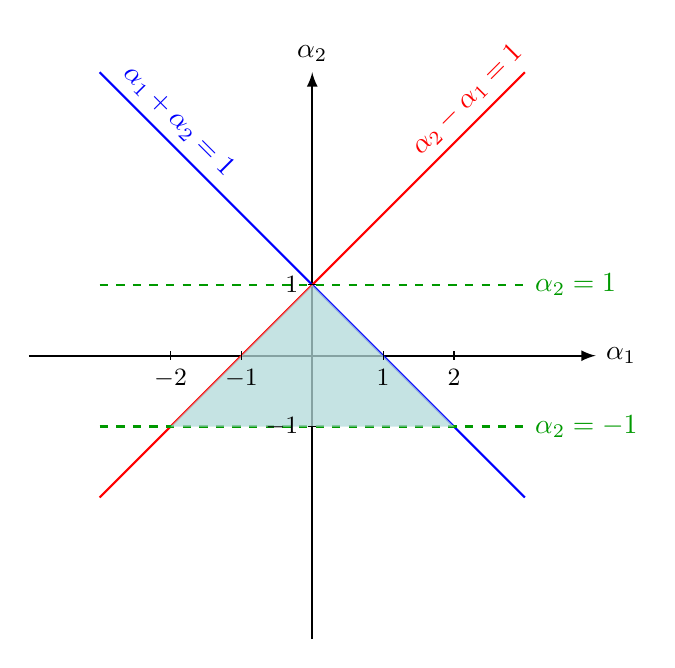
\begin{tikzpicture}[scale=0.9,>=latex]

   % axes
  \draw[->,thick] (-4,0) -- (4,0) node[right] {$\alpha_1$};
  \draw[->,thick] (0,-4) -- (0,4) node[above] {$\alpha_2$};

  % named constraint lines (long segments so intersections occur inside the view)
  \draw[name path=sl1, blue, thick]    (-3,4) -- (3,-2) node[pos=0.15, sloped, above] {$\alpha_1+\alpha_2=1$};
  \draw[name path=sl2, red,  thick]    (-3,-2) -- (3,4)  node[pos=0.90, sloped, above] {$\alpha_2-\alpha_1=1$};
  \draw[name path=top, green!60!black, dashed, thick]    (-3,1)  -- (3,1)  node[right] {$\alpha_2=1$};
  \draw[name path=bottom, green!60!black, dashed, thick] (-3,-1) -- (3,-1) node[right] {$\alpha_2=-1$};

  % compute intersections
  \path[name intersections={of=sl1 and bottom, by=I1}]; % left base: (-2,-1)
  \path[name intersections={of=sl2 and bottom, by=I2}]; % right base: (2,-1)
  \path[name intersections={of=sl1 and top,    by=I3}]; % apex: (0,1)

  % fill feasible triangular region
  \fill[teal!30,opacity=0.75] (I1) -- (I2) -- (I3) -- cycle;

  

  % ticks on axes
  \foreach \x in {-2,-1,1,2} \draw (\x,0.06) -- (\x,-0.06) node[below] {\small $\x$};
  \foreach \y in {-1,1}       \draw (0.06,\y) -- (-0.06,\y) node[left]  {\small $\y$};

\end{tikzpicture}
\end{center}


\bcquestion \hspace{0.1cm} Comment whether the following AR$(2)$ processes are stationary.
\begin{enumerate}[(i)]
\item $X_t - X_{t-1} + \dfrac{1}{4} X_{t-2} = Z_t$
\item $X_t = 0.5 X_{t-1} + 0.7 X_{t-2} + Z_t$
\end{enumerate}

\bccrayon \hspace{0.1cm} We have to identify $\alpha_1$, $\alpha_2$ and then we will check whether they agree with conditions as in (\ref{ar2stationaryconditions}).
\begin{enumerate}[(i)]
\item Given $X_t - X_{t-1} + \dfrac{1}{4} X_{t-2} = Z_t$. Comparing with (\ref{ar2}), $\alpha_1 = 1$, $\alpha_2 = - \dfrac{1}{4}$.

\begin{align*}
\alpha_1 + \alpha_2 &= 1 - \dfrac{1}{4} = \dfrac{3}{4} < 1 \,\, \scalebox{1.5}{\twemoji{check mark button}} \\[0.5em]
\alpha_2 - \alpha_1 &= - \dfrac{1}{4} - 1 = - \dfrac{5}{4} < 1 \,\, \scalebox{1.5}{\twemoji{check mark button}} \\[0.5em]
|\alpha_2| &= \left|-\dfrac{1}{4}\right| = \dfrac{1}{4} < 1 \,\, \scalebox{1.5}{\twemoji{check mark button}}
\end{align*}

So, the given AR$(2)$ process is stationary.

\item Given $X_t = 0.5 X_{t-1} + 0.7 X_{t-2} + Z_t$. Comparing with (\ref{ar2}), $\alpha_1 = 0.5$, $\alpha_2 = 0.7$.

\begin{align*}
\alpha_1 + \alpha_2 = 0.5 + 0.7 = 1.2 \nless 1 \,\, \scalebox{1.5}{\twemoji{double exclamation mark}} 
\end{align*}

So, the given AR$(2)$ process is not stationary.

\end{enumerate}

\newpage

\section{ARMA Process}

A useful class of models for time series is that formed from a combination of MA and AR processes. \\[0.5em]

\subsection{ARMA(p, q) Process}
A process $\{X_t\}$ is said to be a mixed Auto-Regressive Moving Average process of order $(p, q)$ containing $p$ AR terms and $q$ MA terms (abbreviated to an ARMA $(p,q)$ process) if $\{X_t\}$ is \textbf{stationary} and for every $t$,

\begin{align}\label{ARMA}
X_t = \alpha_1 X_{t-1} + \ldots + \alpha_p X_{t-p} + Z_t + \theta_1 Z_{t-1} + \ldots + \theta_q Z_{t-q} \nonumber \\[0.5em]
\text{or } X_t - \alpha_1 X_{t-1} - \ldots - \alpha_p X_{t-p} = Z_t + \theta_1 Z_{t-1} + \ldots + \theta_q Z_{t-q}
\end{align}

where $Z_t \overset{iid}{\sim} \text{White Noise }(0, \sigma^2)$ \& the polynomials $(1 - \alpha_1 z - \alpha_2 z^2 - \ldots - \alpha_p z^p)$ and $(1 + \theta_1 z + \theta_2 z^2 + \ldots + \theta_q z^q)$ do not have any common factors\footnote{The restriction of no common factors is necessary for a unique and minimal representation of the process.}. $\alpha_1, \ldots, \alpha_p$ are AR coefficients and $\theta_1, \ldots, \theta_q$ are MA coefficients. \\[0.5em]

The process $\{X_t\}$ is said to be an \textbf{ARMA} $\boldsymbol{(p,q)}$ \textbf{process with mean} $\boldsymbol{\mu}$ if $\{X_t - \mu\}$ is an ARMA $(p,q)$ process. \\[0.5em]

A more concise representation of (\ref{ARMA}) is
\begin{equation}\label{ARMAbackshift}
\alpha(B) X_t = \theta(B) Z_t
\end{equation}

where $\alpha(\cdot)$ and $\theta(\cdot)$ are polynomials of order $p$ and $q$ respectively such that
\begin{equation}\label{ARpoly}
\alpha(z) = 1 - \alpha_1 z - \alpha_2 z^2 - \ldots - \alpha_p z^p \,\, \forall z \in \mathbb{C}
\end{equation}
and
\begin{equation}\label{MApoly}
\theta(z) = 1 + \theta_1 z + \theta_2 z^2 + \ldots + \theta_q z^q \,\, \forall z \in \mathbb{C}
\end{equation}
and $B$ is a backshift operator such that $B^j X_t = X_{t-j}$, $B^j Z_t = Z_{t-j}$, $\forall j = 0, 1, 2, \ldots$. \\[0.5em]

$\alpha(z)$ as in (\ref{ARpoly}) is called the AR polynomial and $\theta(z)$ as in (\ref{MApoly}) is called the MA polynomial.

\vspace{0.4cm}

\begin{definition}
\textbf{Causality\footnote{That is to say that $X_t$ can be expressed in terms of $Z_s$, $s \leq t$.} :} An ARMA $(p,q)$ process $\{X_t\}$ is \textbf{causal}, or a \textbf{causal function} of $\{Z_t\}$, if there
exist constants $\{\psi_j\}$ such that 
$$\sum \limits_{j=0}^{\infty} |\psi_j| < \infty \quad \text{and} \quad X_t = \sum \limits_{j=0}^{\infty} \psi_j Z_{t-j} \,\, \forall \, t.$$

Causality is equivalent to the condition
$$\alpha(z) = 1 - \alpha_1 z - \cdots - \alpha_p z^p \neq 0 
\quad \forall \, |z| \leq 1.$$
\end{definition}

\vspace{0.4cm}

\begin{definition}
\textbf{Invertibility\footnote{That is to say that $Z_t$ can be expressed in terms of $X_s$, $s \leq t$.} :} An ARMA $(p,q)$ process $\{X_t\}$ is \textbf{invertible} if there exist constants $\{\pi_j\}$ such that
$$\sum \limits_{j=0}^{\infty} |\pi_j| < \infty \quad \text{and} \quad Z_t = \sum \limits_{j=0}^{\infty} \pi_j X_{t-j} \,\, \forall \, t.$$

Invertibility is equivalent to the condition
$$\theta(z) = 1 + \theta_1 z + \cdots + \theta_q z^q \neq 0
\quad \forall \, |z| \leq 1.$$

\end{definition}

$\bullet$ The ARMA $(p, q)$ process as in (\ref{ARMAbackshift}) will be \textbf{causal} and \textbf{stationary} if
\begin{equation}\label{ARMAcausalcondition}
\alpha(z) = 1 - \alpha_1 z - \alpha_2 z^2 - \ldots - \alpha_p z^p \neq 0 \,\, \forall \, |z| \leq 1
\end{equation}
or in other words, all the roots of the AR polynomial (\ref{ARpoly}) have to lie outside the unit circle $|z| = 1$. \\[0.5em]

$\bullet$ The ARMA $(p, q)$ process as in (\ref{ARMAbackshift}) will be \textbf{invertible} if
\begin{equation}\label{ARMAinvertiblecondition}
\theta(z) = 1 + \theta_1 z + \theta_2 z^2 + \ldots + \theta_q z^q \neq 0 \,\, \forall \, |z| \leq 1
\end{equation}
or in other words, all the roots of the MA polynomial (\ref{MApoly}) have to lie outside the unit circle $|z| = 1$. \\[0.5em]

\bcquestion \hspace{0.1cm} Determine which of the following ARMA processes are stationary and / or invertible.
\begin{enumerate}[(i)]
\item $X_t - 0.5 X_{t-1} + 0.06 X_{t-2} = Z_t + 2 Z_{t-1}$
\item $X_t - 1.6 X_{t-1} + 0.6 X_{t-2} = Z_t - \dfrac{10}{3}Z_{t-1} + Z_{t-2}$
\end{enumerate}

\bccrayon \hspace{0.1cm} We have to identify AR and MA polynomials. Then we shall try to check whether the roots of the polynomials lie outside the unit circle or not.

\begin{enumerate}[(i)]
\item Given is an ARMA$(2, 1)$ process with AR polynomial $\alpha(z) = 1 - 0.5 z + 0.06 z^2$ and MA polynomial $\theta(z) = 1 + 2z$. Thus, $\alpha_1 = 0.5, \alpha_2 = -0.06$ and $\theta_1 = 2$.

\begin{align*}
\alpha_1 + \alpha_2 &= 0.5 - 0.06 = 0.44 < 1 \,\, \scalebox{1.5}{\twemoji{check mark button}} \\[0.5em]
\alpha_2 - \alpha_1 &= - 0.06 - 0.5 = - 0.56 < 1 \,\, \scalebox{1.5}{\twemoji{check mark button}} \\[0.5em]
|\alpha_2| &= \left|-0.06\right| = 0.06 < 1 \,\, \scalebox{1.5}{\twemoji{check mark button}}
\end{align*}

AR coefficients agree with conditions (\ref{ar2stationaryconditions}). So, the given ARMA process is \textbf{stationary}. Now
$$1 + 2z = 0 \Rightarrow z = - \dfrac{1}{2} \Rightarrow |z| \leq 1 \,\, \scalebox{1.5}{\twemoji{double exclamation mark}}$$
So, the given ARMA process is \textbf{not invertible}.


\item Given is an ARMA$(2, 2)$ process with AR polynomial $\alpha(z) = 1 - 1.6 z + 0.6 z^2$ and MA polynomial $\theta(z) = 1 - \dfrac{10}{3} z + z^2$. Thus, $\alpha_1 = 1.6, \alpha_2 = -0.6$ and $\theta_1 = \dfrac{10}{3}, \theta_2 = 1$.

\begin{align*}
\alpha_1 + \alpha_2 &= 1.6 - 0.6 = 1 \nless 1 \,\, \scalebox{1.5}{\twemoji{double exclamation mark}}
\end{align*}

AR coefficients do not agree with conditions (\ref{ar2stationaryconditions}). So, the given ARMA process is \textbf{not stationary}. Now
\begin{align*}
1 - \dfrac{10}{3} z + z^2 &= 0 \\[0.2em]
\Rightarrow 3z^2 - 10 z + 3 &= 0 \\[0.2em]
\Rightarrow (z-3) (3z-1) &= 0 \\[0.2em]
\Rightarrow z = 3, \dfrac{1}{3} \Rightarrow |z| \leq 1 \,\, \scalebox{1.5}{\twemoji{double exclamation mark}}
\end{align*}
So, the given ARMA process is \textbf{not invertible}.
\end{enumerate}

\subsection{ARMA(1, 1) Process}

The time series $\{X_t\}$ is an \textbf{ARMA(1,1) process} if it is \textbf{stationary} and satisfies
\begin{equation} \label{ARMA_11}
X_t - \phi X_{t-1} = Z_t + \theta Z_{t-1} \, \forall \, t
\end{equation}

where $\{Z_t\} \sim \text{WN}(0,\sigma^2)$ and $\phi + \theta \neq 0$. Using the backward shift operator $B$, (\ref{ARMA_11}) can be written more concisely as
\begin{equation} \label{ARMA_11_concise}
\phi(B)X_t = \theta(B)Z_t
\end{equation}

where $\phi(B)$ and $\theta(B)$ are the linear filters $\phi(B) = 1 - \phi B$ and $\theta(B) = 1 + \theta B$ respectively. \\[0.2em]

We first investigate the range of values of $\phi$ and $\theta$ for which a stationary solution of (\ref{ARMA_11}) exists. If $|\phi| < 1$, let $\chi(z)$ denote the power series expansion of $1/\phi(z)$, i.e.,
$\sum \limits_{j=0}^{\infty} \phi^j z^j$ which has absolutely summable coefficients. Then $\chi(B)\phi(B) = 1$. Applying $\chi(B)$ to each side of (\ref{ARMA_11_concise}) therefore gives
$$X_t = \chi(B)\theta(B)Z_t = \psi(B)Z_t$$
where
$$\psi(B) = \sum \limits_{j=0}^{\infty} \psi_j B^j = (1 + \phi B + \phi^2 B^2 + \ldots)(1 + \theta B).$$

By multiplying out the right-hand side, we find that
$$\psi_0 = 1 \quad \text{and} \quad \psi_j = (\phi + \theta)\phi^{j-1}
\quad \text{for } j \geq 1.$$

We conclude that the MA$(\infty)$ process
\begin{equation} \label{ARMA_11_stationary_solution}
X_t = Z_t + (\phi + \theta)\sum \limits_{j=1}^{\infty} \phi^{j-1} Z_{t-j}
\end{equation}
is the unique stationary solution of (\ref{ARMA_11}). A stationary solution of the ARMA$(1,1)$ equations exists if and only if $\phi \neq \pm 1$. If $|\phi| < 1$, then the unique stationary solution is given by (\ref{ARMA_11_stationary_solution}). In this case we say that $\{X_t\}$ is \textbf{causal} or a causal function of $\{Z_t\}$, since $X_t$ can be expressed in terms of the current and past values $Z_s$, $s \leq t$. If $|\phi| > 1$, then the unique stationary solution is \textbf{noncausal}. \\[0.2em]

The ARMA$(1,1)$ process defined by (\ref{ARMA_11}) is \textbf{invertible} if $|\theta| < 1$. To demonstrate this, let $\xi(z)$ denote the power series expansion of $1/\theta(z)$, i.e., $\sum \limits_{j=0}^{\infty} (-\theta)^j z^j,$ which has absolutely summable coefficients. Then $\xi(B)\theta(B) = 1$, and applying $\xi(B)$ to each side of (\ref{ARMA_11_concise}) gives
$$Z_t = \xi(B)\phi(B)X_t = \pi(B)X_t,$$
where
$$\pi(B) = \sum \limits_{j=0}^{\infty} \pi_j B^j = (1 - \theta B + (-\theta)^2 B^2 + \ldots)(1 - \phi B).$$

By multiplying out the right-hand side, we find that
\begin{equation}
Z_t = X_t - (\phi + \theta)\sum \limits_{j=1}^{\infty} (-\theta)^{\,j-1} X_{t-j}.
\end{equation}

Thus the ARMA$(1,1)$ process is \textbf{invertible}, since $Z_t$ can be expressed in terms of the present and past values of the process $X_s$, $s \leq t$.

\subsubsection{ACVF for ARMA(1, 1) Process}

For a \textit{stationary} ARMA$(1, 1)$ process, multiplying both side of (\ref{ARMA_11}) by $X_{t-h}$, $h = 0, 1, 2, \ldots$ and taking expectations we get

\begin{align}
\text{for } h = 0; \,\, &\gamma(0) - \phi \gamma(1) = \sigma^2 + \theta (\phi + \theta) \sigma^2, \\[0.2em]
\text{for } h = 1; \,\, &\gamma(1) - \phi \gamma(0) = \theta \sigma^2, \label{ARMA_11_YW_h_1}\\[0.2em]
\text{for } h \geq 2; \,\, &\gamma(h) - \phi \gamma(h-1) = 0. \label{ARMA_11_YW_h_geq_2}
\end{align}

From (\ref{ARMA_11_stationary_solution}),

\begin{align*}
\gamma(0) &= \sigma^2 \left[ 1 + (\phi + \theta)^2 \sum \limits_{j = 0}^{\infty} \phi^{2j} \right] \\[0.35em]
&= \sigma^2 \left[ 1 + \dfrac{(\theta + \phi)^2}{1 - \phi^2} \right].
\end{align*}

From (\ref{ARMA_11_YW_h_1}),
\begin{align*}
\gamma(1) &= \theta \sigma^2 + \phi \sigma^2 \left[ 1 + \dfrac{(\theta + \phi)^2}{1 - \phi^2} \right] \\[0.35em]
&= \sigma^2 \left[ \theta + \phi + \dfrac{(\theta + \phi)^2\phi}{1 - \phi^2} \right].
\end{align*}

Thus, from (\ref{ARMA_11_YW_h_geq_2}),
\begin{align*}
\gamma(h) = \phi^{h-1} \gamma(1), \,\, \forall \, h \geq 2.
\end{align*}
\newpage

\section{Estimation of Mean and Autocorrelation Function of a Stationary Process}

A stationary process $\{X_t\}$ is characterized, at least from a second-order point of view, by its mean $\mu$ and its auto-covariance function $\gamma(\cdot)$. The estimation of $\mu$, $\gamma(\cdot)$, and the auto-correlation function $\rho(\cdot) = \gamma(\cdot)/\gamma(0)$ from observations $X_1,\ldots, X_n$ therefore plays a crucial role in problems of inference and in particular in the problem of constructing an appropriate model for the data.

\subsection{Estimation of $\mu$}

The moment estimator of the mean $\mu$ of a stationary process is the sample mean
\begin{align*}
\bar{X_n} = \dfrac{1}{n} \sum \limits_{i = 1}^{n} X_i
\end{align*}

$\bar{X_n}$ is also an unbiased estimator of $\mu$ since $E(\bar{X_n}) = \mu$ $\forall$ $\mu$ in the parameter space. \\[0.25em]

The mean squared error of $\bar{X_n}$ is
\begin{align}\label{msestationary}
E(\bar{X_n} - \mu)^2 &= \text{var}(\bar{X_n}) \nonumber \\[0.25em]
&= \dfrac{1}{n^2} \sum \limits_{i = 1}^{n} \sum \limits_{j = 1}^{n} \text{cov}(X_i, X_j)
\end{align}

$\{X_t\}$ is a Second order stationary process, so covariances depend only on lag $h$. At lag $h$, covariance is $\gamma(h)$. In (\ref{msestationary}), there are $n^2$ covariance terms; but the only possible values of absolute lag $|h|$ are $0, 1, 2, \ldots, n-1$. So it suffices to count how many times each of the $|h|$'s occur. Initially we will try to count the occurrence of a few $|h|$'s and then we will try to generalize the idea. \textit{In the following discussion, whenever it is mentioned that there are 2 occurrences of $|h| = x$, it is surely the case that $h = -x$ occurs once and $h = x$ occurs once.}

\begin{itemize}
\item Clearly, lag $h = 0$ occurs exactly $n$ times. Each $X_i$ has lag $0$ with itself only.
\item Except the $2$ boundaries $X_1$ and $X_n$, all of $X_2, X_3, \ldots, X_{n-2}, X_{n-1}$ create $2$ occurrences of $|h| = 1$; \textit{e.g.} $X_2$ has $|h| = 1$ with $X_1$ and $X_3$, $X_3$ has $|h| = 1$ with $X_2$ and $X_4$. $X_1$, $X_n$ create only one occurrence of $|h| = 1$ with $X_2$ and $X_{n-1}$ respectively. So in total, there are $2(n-2) + 2 = 2n - 2 = 2(n-1)$ occurrences of $|h| = 1$.
\item Except the $4$ extremes $X_1$, $X_2$, $ँँँँँँँंंX_{n-1}$, $X_n$, all of $X_3, X_4, \ldots, X_{n-3}, X_{n-2}$ create $2$ occurrences of $|h| = 2$; \textit{e.g.} $X_3$ has $|h| = 2$ with $X_1$ and $X_5$, $X_4$ has $|h| = 2$ with $X_2$ and $X_6$. $X_1$, $X_2$, $ँँँँँँँंंX_{n-1}$, $X_n$ create only one occurrence of $|h| = 2$ with $X_3$, $X_4$, $ँँँँँँँंंX_{n-3}$, $X_{n-2}$ respectively. So in total, there are $2(n-4) + 4 = 2n - 4 = 2(n - 2)$ occurrences of $|h| = 2$.
\item Except the $6$ extremes $X_1$, $X_2$, $X_3$, $X_{n-2}$, $ँँँँँँँंंX_{n-1}$, $X_n$, all of $X_4, X_5, \ldots, X_{n-4}, X_{n-3}$ create $2$ occurrences of $|h| = 3$; \textit{e.g.} $X_4$ has $|h| = 3$ with $X_1$ and $X_7$, $X_5$ has $|h| = 2$ with $X_2$ and $X_8$. $X_1$, $X_2$, $X_3$, $X_{n-2}$, $ँँँँँँँंंX_{n-1}$, $X_n$ create only one occurrence of $|h| = 3$ with $X_4$, $X_5$, $X_6$, $X_{n-5}$, $ँँँँँँँंंX_{n-4}$, $X_{n-3}$ respectively. So in total, there are $2(n-6) + 6 = 2n - 6 = 2(n - 3)$ occurrences of $|h| = 3$.
\item In general, there are $n$ occurrences of $|h| = 0$, $2(n - |h|)$ occurrences of $|h|$ $\forall |h| = 1(1)\overline{n-1}$ and at each occurrence the covariance is $\gamma(|h|) = \gamma(h)$. So, in total there are $2 \cdot \dfrac{n(n-1)}{2} + n = n^2$ many covariance terms.
\end{itemize}

Thus from (\ref{msestationary}) it follows
\begin{align}\label{msestationarycontinued}
\text{var}(\bar{X_n}) &= \dfrac{1}{n^2} \sum \limits_{i = 1}^{n} \sum \limits_{j = 1}^{n} \text{cov}(X_i, X_j) \nonumber \\[0.25em]
&= \dfrac{1}{n^2} \left[ n\gamma(0) + \sum \limits_{|h| = 1}^{n-1} 2(n - |h|) \gamma(h) \right] \nonumber \\[0.25em]
&= \dfrac{1}{n^2} \left[ (n - 0)\gamma(0) + \sum \limits_{\substack{h = -(n-1) \\[4pt] h \neq 0}}^{n-1} (n - |h|) \gamma(h) \right] \nonumber \\[0.25em]
&= \dfrac{1}{n^2} \sum \limits_{h = -(n-1)}^{n-1} (n - |h|) \gamma(h) \nonumber \\[0.25em]
&= \dfrac{1}{n} \sum \limits_{h = -(n-1)}^{n-1} \left(1 - \dfrac{|h|}{n}\right) \gamma(h)
\end{align}

If $\gamma(n) \rightarrow 0$ as $n \rightarrow \infty$, then  (\ref{msestationarycontinued}) converges to $0$ so that by the sufficient conditions of consistency, $\bar{X_n}$ converges to $\mu$. In other words, $\bar{X_n}$ is a consistent estimator of $\mu$. \\[0.25em]

If $\sum \limits_{h = -\infty}^{\infty} |\gamma(h)| < \infty$, then $\lim \limits_{n \rightarrow \infty} n \, \text{var}(\bar{X_n}) = \sum \limits_{|h| < \infty} \gamma(h)$. \\[0.25em]

If the time series is Gaussian, then $\sqrt{n}\left( \bar{X_n} - \mu \right) \sim N \left( 0, \sum \limits_{|h| < n} \left(1 - \dfrac{|h|}{n}\right) \gamma(h) \right)$. In other cases, we approximate $\sqrt{n}\left( \bar{X_n} - \mu \right) \sim N \left( 0,  \sum \limits_{|h| < \infty} \gamma(h) \right)$ for large $n$. \\[0.25em]

An approximate $95\%$ confidence interval for $\mu$ is given by
\begin{align*}
\left( \bar{X_n} - 1.96 \cdot \sqrt{\dfrac{v}{n}}, \bar{X_n} + 1.96 \cdot \sqrt{\dfrac{v}{n}} \right)
\end{align*}
where $v = \sum \limits_{|h| < \infty} \gamma(h)$. Of course, $v$ is not generally known, so it must be estimated from the data. \\[0.25em]

$\bullet$ An example : Consider an AR$(1)$ process $\{X_t\}$ with mean $\mu$ defined by the equation
\begin{equation*}
X_t - \mu = \alpha \left( X_{t-1} - \mu \right) + Z_t
\end{equation*}
where $|\alpha| < 1$ and $Z_t \sim \text{White Noise } (0, \sigma^2)$. \\[0.25em]

For AR$(1)$ process, $\gamma(h) = \dfrac{\sigma^2 \alpha^{|h|}}{1-\alpha^2}$. \\[0.25em]

Then 
\begin{align*}
v &= \sum \limits_{|h| < \infty} \gamma(h) \\[0.25em]
&= \sum \limits_{|h| < \infty} \dfrac{\sigma^2 \alpha^{|h|}}{1-\alpha^2} \\[0.25em]
&= \dfrac{\sigma^2}{1-\alpha^2} + 2\sum \limits_{h = 1}^{\infty} \dfrac{\sigma^2 \alpha^h}{1-\alpha^2} \\[0.25em]
&= \dfrac{\sigma^2}{1-\alpha^2} + \dfrac{2\sigma^2}{1-\alpha^2} \sum \limits_{h = 1}^{\infty} \alpha^h \\[0.25em]
&= \dfrac{\sigma^2}{1-\alpha^2} + \dfrac{2\sigma^2}{1-\alpha^2} \cdot \dfrac{\alpha}{1-\alpha} \\[0.25em]
&= \dfrac{\sigma^2}{1-\alpha^2} \left( 1 + \dfrac{2\alpha}{1-\alpha} \right) \\[0.25em]
&= \dfrac{\sigma^2}{1-\alpha^2} \left( \dfrac{1 - \alpha + 2\alpha}{1-\alpha} \right) \\[0.25em]
&= \dfrac{\sigma^2}{1-\alpha^2} \left( \dfrac{1 + \alpha}{1 - \alpha} \right) \\[0.25em]
&= \dfrac{\sigma^2}{(1-\alpha)^2}
\end{align*}

Approximate $95\%$ confidence interval for $\mu$ is given by 
\begin{align*}
\left( \bar{X_n} - \dfrac{1.96}{\sqrt{n}} \cdot \dfrac{\sigma}{1-\alpha}, \bar{X_n} + \dfrac{1.96}{\sqrt{n}} \cdot \dfrac{\sigma}{1-\alpha} \right)
\end{align*}

In practice, $\sigma$ and $\alpha$ are unknown, so in the confidence interval they must be replaced by their estimates.

\subsection{Estimation of $\gamma(\cdot)$ and $\rho(\cdot)$}

Let $X_1, X_2, \ldots, X_n$ be observations from a stationary process $\{X_t\}$ with autocovariance function $\gamma(\cdot)$ and autocorrelation function $\rho(\cdot)$. \\[0.25em]

The sample autocovariance function $\hat{\gamma}(\cdot)$ is defined by
\begin{equation}\label{sampleautocovariance}
\hat{\gamma}(h) = \dfrac{1}{n} \sum \limits_{t = 1}^{n - |h|} \left( X_{t+|h|} - \bar{X_n} \right) \left( X_t - \bar{X_n} \right)
\end{equation}
and the sample autocorrelation function $\hat{\rho}(\cdot)$ is defined by
\begin{equation}\label{sampleautocorrelation}
\hat{\rho}(h) = \dfrac{\hat{\gamma}(h)}{\hat{\gamma}(0)}.
\end{equation}

Both the estimators $\hat{\gamma}(h)$ and $\hat{\rho}(h)$ are biased even if the denominator in (\ref{sampleautocovariance}) is replaced by $n-h$. Nevertheless, under general assumptions they are nearly unbiased for large sample sizes. \\[0.25em]

The sample ACVF has the desirable property that for each $k \geq 1$ the $k-$dimensional sample covariance matrix

\begin{align*}
\hat{\Gamma}_k =
\begin{bmatrix}
\hat{\gamma}(0) & \hat{\gamma}(1) & \ldots & \hat{\gamma}(k-1) \\
\hat{\gamma}(1) & \hat{\gamma}(0) & \ldots & \hat{\gamma}(k-2) \\
\vdots & \vdots & \ddots & \vdots \\
\hat{\gamma}(k-1) & \hat{\gamma}(k-2) & \ldots & \hat{\gamma}(0)
\end{bmatrix}
\end{align*}

is non-negative definite. \\[0.25em]

The sample autocorrelation matrix
\begin{align*}
\hat{R}_k = \dfrac{\hat{\Gamma}_k}{\hat{\gamma}(0)} = 
\begin{bmatrix}
1 & \hat{\rho}(1) & \ldots & \hat{\rho}(k-1) \\
\hat{\rho}(1) & 1 & \ldots & \hat{\rho}(k-2) \\
\vdots & \vdots & \ddots & \vdots \\
\hat{\rho}(k-1) & \hat{\rho}(k-2) & \ldots & 1
\end{bmatrix}
\end{align*}

is also non-negative definite\footnote{Replacing $n$ by $n-h$ in the definition of $\hat{\gamma}(h)$ (\ref{sampleautocovariance}) may not ensure resulting $\hat{\Gamma}(k)$ and $\hat{R}(k)$ to be non-negative definite.}. To see this, first note that if $\hat{\Gamma}_m$ is non-negative definite, then $\hat{\Gamma}_k$ is non-negative definite $\forall$ $k < m$. So assume $k \geq n$ and write

$$\hat{\Gamma}_k = n^{-1}TT'$$

where $T$ is the $k \times 2k$ matrix
$$T =
\begin{bmatrix}
0 & \cdots & 0 & 0 & Y_1 & Y_2 & \cdots & Y_k \\
0 & \cdots & 0 & Y_1 & Y_2 & \cdots & Y_k & 0 \\
\vdots &  & \vdots & \vdots & \vdots &  & \vdots & \vdots \\
0 & Y_1 & Y_2 & \cdots & Y_k & 0 & \cdots & 0
\end{bmatrix},
$$

where $Y_i = X_i - \bar{X}_n$, $i = 1, \dots, n,$ and $Y_i = 0$ for $i = n+1, \dots, k.$ Then for any real $k \times 1$ vector $\utilde{a}$ we have
$$ \utilde{a}' \hat{\Gamma}_k \utilde{a} = n^{-1}(\utilde{a}'T)(T'\utilde{a}) = n^{-1} ||T'\utilde{a}||^2 \geq 0.$$

Thus $\hat{\Gamma}_k$ and $\hat{R}_k$ are non-negative definite. \\[0.25em]

$\bullet$  The sample ACF plays an important role in the selection of suitable models for the data. For systematic inference concerning $\rho(h)$ we need the sampling distribution of the estimator $\hat{\rho}(h)$. Although the distribution of $\hat{\rho}(h)$ is intractable for samples from even the simplest time series models, it can usually be well approximated by a normal distribution for large sample sizes. For linear models and in particular for ARMA models, it can be established that 
$$\utilde{\hat{\rho_k}} = \left( \hat{\rho}(1), \hat{\rho}(2), \ldots, \hat{\rho}(k)\right)'$$ 
is approximately distributed as $N_k\left( \utilde{\rho_k}, \dfrac{W}{n} \right)$ for large $n$ \textit{i.e.} 
\begin{align}\label{largesampledistributionofsampleacfs}
\utilde{\hat{\rho_k}} \approx N_k\left( \utilde{\rho_k}, \dfrac{W}{n} \right)
\end{align}
where $\utilde{\rho_k} = \left( \rho(1), \rho(2), \ldots, \rho(k) \right)'$ and $W$ is the covariance matrix whose $(i, j)$th element is given by \textbf{Bartlett's Formula}
\begin{equation}\label{bartlettsformula}
w_{ij} = \sum \limits_{h = 1}^{\infty} \{\rho(h+i) + \rho(h-i) - 2\rho(h)\rho(i)\} \times \{\rho(h+j) + \rho(h-j) - 2\rho(h)\rho(j)\}.
\end{equation}

\subsubsection{For a Purely Random Process}

Let $\{X_t\} \sim \text{White Noise }(0, \sigma^2)$. Then $\rho(h) = \begin{cases}1, &h=0 \\ 0, &\text{otherwise}\end{cases}$.\\[0.25em]

$i, j > 0$. When $h = i \neq j$, $\{\rho(h+j) + \rho(h-j) - 2\rho(h)\rho(j)\} = 0$, alternatively when $h = j \neq i$, $\{\rho(h+i) + \rho(h-i) - 2\rho(h)\rho(i)\} = 0$. Only when $h = i = j > 0$, exactly one term in the summation as in (\ref{bartlettsformula}) is non-zero and rest all terms are $0$. The non-zero term is $\{\rho(2i) + \rho(0) - 2\rho(i)^2\}^2 = (0 + 1 - 0)^2 = 1$. \\[0.25em]

Thus from (\ref{bartlettsformula}), $w_{ij} = \begin{cases}1, &i = j \\ 0, &\text{otherwise}\end{cases}$. \\[0.25em]

So, for large $n$, $\hat{\rho}(1), \hat{\rho}(2), \ldots, \hat{\rho}(h) \overset{iid}{\approx} N\left(0, \dfrac{1}{n}\right)$. \\[0.25em]

Approximate $95\%$ confidence interval for $\hat{\rho}(h)$ is given by
$\left(-1.96 \cdot \dfrac{1}{\sqrt{n}}, 1.96 \cdot \dfrac{1}{\sqrt{n}}\right).$

\subsubsection{For an MA(1) Process}

Let $\{X_t\}$ be an MA$(1)$ process as in (\ref{ma1thetarepresentation}) \textit{i.e.} $X_t = Z_t + \theta Z_{t-1}, \,\, t = 0, \pm 1, \pm 2, \ldots$ and $Z_t \sim \text{White Noise }(0, \sigma^2).$\\[0.25em]

We have
\begin{align*}
\rho(h) &= \begin{cases}
1, \,\, h = 0 \\[0.25em]
\dfrac{\theta}{1 + \theta^2}, \,\, h = \pm 1 \\[0.5em]
0, \,\, h = \pm 2, \pm 3, \pm 4, \ldots
\end{cases}
\end{align*}

Again $\displaystyle{w_{ii} = \sum \limits_{h = 1}^{\infty} \{\rho(h+i) + \rho(h-i) - 2\rho(h)\rho(i)\}^2}$. \\[0.25em]

Now,
\begin{align}
w_{11} &= \sum \limits_{h = 1}^{\infty} \{\rho(h+1) + \rho(h-1) - 2\rho(h)\rho(1)\}^2 \nonumber \\[0.25em]
&= \left[\rho(2) + \rho(0) - 2\rho(1)^2\right]^2 + \left[\rho(3) + \rho(1) - 2\rho(2)\rho(1)\right]^2 + \sum \limits_{h = 3}^{\infty} \{\rho(h+1) + \rho(h-1) - 2\rho(h)\rho(1)\}^2 \nonumber \\[0.25em]
&= \left[\underbrace{\rho(2)}_{0} + \rho(0) - 2\rho(1)^2\right]^2 + \left[\underbrace{\rho(3)}_{0} + \rho(1) - 2\underbrace{\rho(2)}_{0}\rho(1)\right]^2 + \underbrace{\sum \limits_{h = 3}^{\infty} \{\rho(h+1) + \rho(h-1) - 2\rho(h)\rho(1)\}^2}_{0} \nonumber \\[0.25em]
&= \left[\rho(0) - 2\rho(1)^2\right]^2 + \left[\rho(1)\right]^2 \nonumber \\[0.25em]
&= \underbrace{\rho(0)^2}_{1} + 4\rho(1)^4 - 4\underbrace{\rho(0)}_{1}\rho(1)^2 + \rho(1)^2 \nonumber \\[0.25em]
&= 1 - 3\rho(1)^2 + 4\rho(1)^4 \label{w_11forMA1}
\end{align}

Again, for any $i > 1$, $\rho(h + i) = 0 \,\, \forall h \geq 1$; $\rho(h - i) = \begin{cases} \rho(-1), &h = i-1 \\ \rho(0), &h = i \\ \rho(1), &h = i+1 \\ 0, &\text{otherwise} \end{cases}$; and $\rho(i) = 0 \,\, \forall i > 1$. \\[0.25em]

$\therefore \, \forall i > 1$, 
\begin{align*}
w_{ii} &= \sum \limits_{h = 1}^{\infty} \{\underbrace{\rho(h+i)}_{0} + \underbrace{\rho(h-i)}_{\neq 0 \text{ only 3 times}} - 2\rho(h)\underbrace{\rho(i)}_{0}\}^2 \\[0.25em]
&= \rho(-1)^2 + \rho(0)^2 + \rho(1)^2 \\[0.25em]
&= 1 + 2\rho(1)^2
\end{align*}

$\therefore w_{ii} = \begin{cases}1 - 3\rho(1)^2 + 4\rho(1)^4, &i = 1 \\ 1 + 2\rho(1)^2, &i > 1 \end{cases}$. \\[0.5em]

Thus, for large $n$, $\hat{\rho}(1) \approx N\left( \rho(1), \dfrac{w_{11}}{n}\right)$ and $\hat{\rho}(k) \approx N\left( \rho(k) = 0, \dfrac{w_{kk}}{n}\right)\,\, \forall k > 1$.

\newpage

\fcLittleMouse[scale = 0.4, draw = brown, line width = 1.5] \textbf{A Practical Example}\footnote{R Program : \href{https://raw.githubusercontent.com/sakunisgithub/Time_Series_Analysis/refs/heads/master/R_Programs/sample_ACF_of_MA_1.R}{sample\_ACF\_of\_MA\_1.R}} : We simulated $n = 200$ observations from MA$(1)$ model $X_t = Z_t - 0.8 Z_{t-1}$. Theoretical $\rho(1) = \dfrac{-0.8}{1 + 0.64} = -0.4878$. From data, $\hat{\rho}(1) = -0.4739862$. We also observed $\forall h = 2(1)40$, $|\hat{\rho}(h)| \leq \dfrac{1.96}{\sqrt{n}}$ which strongly suggests that the data are from a model in which observations are uncorrelated past lag 1. \\[0.25em]

We also use the bounds $\pm \dfrac{1.96}{\sqrt{n}}\sqrt{1 + 2\rho(1)^2}$ to check compatibility of the data with the model $X_t = Z_t - 0.8 Z_{t-1}$. \\[0.25em]

However, $\rho(1)$ is not generally known in advance. So we compare autocorrelations $\hat{\rho}(2), \hat{\rho}(3), \ldots, \hat{\rho}(40)$ with the bounds $\pm \dfrac{1.96}{\sqrt{n}}\sqrt{1 + 2\hat{\rho}(1)^2}$ in order to check the hypothesis that the data are generated by a moving-average process of order 1. \\[0.25em]

Here is a plot with $\hat{\rho}(1), \hat{\rho}(2), \hat{\rho}(3), \ldots, \hat{\rho}(40)$, $\pm \dfrac{1.96}{\sqrt{n}}$ bounds (in red) and $\pm \dfrac{1.96}{\sqrt{n}}\sqrt{1 + 2\hat{\rho}(1)^2}$ bounds (in green).

\begin{figure}[!htbp]
\centering
\includegraphics[scale=0.4]{figures/sample_ACF_of_MA_1.png}
\end{figure}

Finally, $95\%$ confidence interval for $\rho(1)$ given by 
\begin{align*}
\Bigg(\hat{\rho}(1) - \dfrac{1.96}{\sqrt{200}}\sqrt{1 - 3\hat{\rho(1)}^2 + 4\hat{\rho(1)}^4} &, \hat{\rho}(1) + \dfrac{1.96}{\sqrt{200}}\sqrt{1 - 3\hat{\rho(1)}^2 + 4\hat{\rho(1)}^4}\Bigg) \\[0.25em]
\Rightarrow \Bigg(\hat{\rho}(1) - \dfrac{1.96}{\sqrt{200}}\sqrt{0.527905} &, \hat{\rho}(1) + \dfrac{1.96}{\sqrt{200}}\sqrt{0.527905}\Bigg) \\[0.25em]
\Rightarrow (-0.4739862 - 0.1006976 &, -0.4739862 + 0.1006976) \\[0.25em]
\Rightarrow (-0.5746838 &, -0.3732886)
\end{align*}
which contains $\rho(1) = -0.4878$.  This further supports the compatibility of the data with the model $X_t = Z_t - 0.8 Z_{t-1}$.

\subsubsection{For an AR(1) Process}

Let $\{X_t\}$ be a AR$(1)$ process as in (\ref{ar1}) \textit{i.e.} $X_t = \alpha X_{t-1} + Z_{t}, \,\, t = 0, \pm 1, \pm 2, \ldots$, $|\alpha| < 1$ and $Z_t \sim \text{White Noise }(0, \sigma^2).$\\[0.25em]

We have $\rho(h) = \alpha^{|h|}, \,\, h = 0, \pm 1, \pm 2, \ldots$.

\begin{align*}
\therefore w_{ii} &= \sum \limits_{h = 1}^{\infty} \{\rho(h+i) + \rho(h-i) - 2\rho(h)\rho(i)\}^2 \\[0.25em]
&= \sum \limits_{h = 1}^{\infty} \{\alpha^{|h+i|} + \alpha^{|h-i|} - 2\alpha^{|h|}\alpha^{|i|}\}^2 \\[0.25em]
&= \sum \limits_{h = 1}^{\infty} \{\alpha^{h+i} + \alpha^{|h-i|} - 2\alpha^{h}\alpha^{i}\}^2, \text{ now we will split the sum into 2 parts } h \leq i \, \& \, h > i \text{ to tackle }|h-i| \\[0.25em]
&= \sum \limits_{h = 1}^{i} \{\alpha^{h+i} + \alpha^{i-h} - 2\alpha^{h}\alpha^{i}\}^2 + \sum \limits_{h = i+1}^{\infty} \{\alpha^{h+i} + \alpha^{h-i} - 2\alpha^{h}\alpha^{i}\}^2 \\[0.25em]
&= \sum \limits_{h = 1}^{i} \alpha^{2i} \{\alpha^{h} + \alpha^{-h} - 2\alpha^{h}\}^2 + \sum \limits_{h = i+1}^{\infty} \alpha^{2h}\{\alpha^{i} + \alpha^{-i} - 2\alpha^{i}\}^2 \\[0.25em]
&= \sum \limits_{h = 1}^{i} \alpha^{2i} \{\alpha^{-h} - \alpha^{h}\}^2 + \sum \limits_{h = i+1}^{\infty} \alpha^{2h}\{\alpha^{-i} - \alpha^{i}\}^2 \\[0.25em]
&= \sum \limits_{h = 1}^{i} \alpha^{2i} \{\alpha^{-2h} + \alpha^{2h} - 2\} + \{\alpha^{-i} - \alpha^{i}\}^2 \sum \limits_{h = i+1}^{\infty} \alpha^{2h} \\[0.25em]
&= \alpha^{2i} \sum \limits_{h = 1}^{i} \{\alpha^{-2h} + \alpha^{2h} - 2\} + \{\alpha^{-i} - \alpha^{i}\}^2 \sum \limits_{h = i+1}^{\infty} \alpha^{2h} \\[0.25em]
&= \alpha^{2i} \sum \limits_{h = 1}^{i} \alpha^{-2h} + \alpha^{2i} \sum \limits_{h = 1}^{i} \alpha^{2h} - \alpha^{2i} \sum \limits_{h = 1}^{i} 2 + \{\alpha^{-i} - \alpha^{i}\}^2 \sum \limits_{h = i+1}^{\infty} \alpha^{2h} \\[0.35em]
&= \alpha^{2i} \cdot \dfrac{\alpha^{-2} (1 - \alpha^{-2i})}{1 - \alpha^{-2}} + \alpha^{2i} \cdot \dfrac{\alpha^{2} (\alpha^{2i} - 1)}{\alpha^{2} - 1} - 2i \alpha^{2i} + \{\alpha^{-i} - \alpha^{i}\}^2 \cdot \dfrac{\alpha^{2(i+1)}}{1-\alpha^{2}} \\[0.35em]
&= \dfrac{\alpha^{2i} (1 - \alpha^{-2i})}{\alpha^{2} -  1} + \dfrac{\alpha^{2(i+1)} (1 - \alpha^{2i})}{1 - \alpha^{2}} - 2i \alpha^{2i} + \dfrac{(\alpha^{-2i} + \alpha^{2i} - 2)\alpha^{2(i+1)}}{1-\alpha^{2}} \\[0.35em]
&= \dfrac{(1 - \alpha^{2i})}{1 - \alpha^{2}} + \dfrac{\alpha^{2(i+1)} (1 - \alpha^{2i})}{1 - \alpha^{2}} + \dfrac{(\alpha^{-2i} + \alpha^{2i} - 2)\alpha^{2(i+1)}}{1-\alpha^{2}} - 2i \alpha^{2i}  \\[0.35em]
&= \dfrac{1 - \alpha^{2i} + \textcolor{blue}{\alpha^{2(i+1)}} - \textcolor{red}{\alpha^{2(i+1)}\alpha^{2i}} + \alpha^{-2i}\alpha^{2(i+1)} + \textcolor{red}{\alpha^{2i}\alpha^{2(i+1)}} - \textcolor{blue}{2\alpha^{2(i+1)}}}{1 - \alpha^{2}} - 2i \alpha^{2i}  \\[0.35em]
&= \dfrac{1 - \alpha^{2i} - \alpha^{2(i+1)} + \alpha^{2}}{1 - \alpha^{2}} - 2i \alpha^{2i} \\[0.35em]
&= \dfrac{1 - \alpha^{2i} + \alpha^{2} - \alpha^{2i}\alpha^{2}}{1 - \alpha^{2}} - 2i \alpha^{2i} \\[0.35em]
&= \dfrac{1 - \alpha^{2i} + \alpha^{2} (1 - \alpha^{2i})}{1 - \alpha^{2}} - 2i \alpha^{2i} \\[0.35em]
&= \dfrac{(1 - \alpha^{2i}) (1  + \alpha^{2})}{1 - \alpha^{2}} - 2i \alpha^{2i}
\end{align*}

$\therefore$ For large $n$, $\hat{\rho}(k) \approx N\left( \rho(k), \dfrac{w_{kk}}{n} \right)$ $\forall k$.

\newpage

\section{The Partial Autocorrelation Function}

The partial autocorrelation function, like the autocorrelation function, conveys vital information regarding the dependence structure of a stationary process. Like the autocorrelation function it also depends only on the second order properties of the process. The partial autocorrelation $\alpha(k)$ at lag $k$ may be regarded as the correlation between $X_1$ and $X_{k+1}$, adjusted for the intervening 
observations $X_2, X_3, \ldots, X_k$.

\begin{definition}\label{PACFdefinition1}
The partial autocorrelation function (PACF) $\alpha(\cdot)$ of a stationary time series $\{X_t\}$ is defined by
$$\alpha(1) = corr(X_2, X_1) = \rho(1)$$
and
$$\alpha(k) = corr(X_{k+1} - \widehat{X_{k+1}}, X_1 - \widehat{X_1}) \,\, \forall k \geq 2$$
where $\widehat{X_{k+1}}$ and $\widehat{X_1}$ are regressions of $X_{k+1}$ and $X_1$ on the intermediate observations $X_2, X_3, \ldots, X_k$.
\end{definition}

The value $\alpha(k)$ is known as the partial autocorrelation at lag $k$. Thus the partial autocorrelation $\alpha(k), \, k \geq 2$, is the correlation of the two residuals obtained after regressing $X_{k+1}$ and $X_1$ on the intermediate observations $X_2, X_3, \ldots, X_k$.

\begin{result}\label{ARbestmeansquarepredictorresult}
If $X_t = \phi_1 X_{t-1} + \phi_2 X_{t-2} + \cdots + \phi_p X_{t-p} + Z_t, \quad t = 0, \pm 1, \ldots,$ where $\{Z_t\}$ is a sequence of uncorrelated random variables, each with mean zero and variance $\sigma^2$, and such that $Z_t$ is uncorrelated with $\{X_j, j < t\}$ for each $t$, the best mean square predictor of $X_{n+1}$ in $\overline{\mathrm{sp}}\{X_j, -\infty < j \le n\}$ is
$$\widehat{X_{n+1}} = \phi_1 X_n + \phi_2 X_{n-1} + \ldots + \phi_p X_{n+1-p}.$$
\end{result}

\subsection{PACF of an AR(1) Process} \label{AR1_PACF}

Consider a stationary AR$(1)$ process as in (\ref{ar1}) with $|\alpha| < 1$. 
Then
\begin{align*}
\alpha(1) &= corr(X_2, X_1) \\[0.25em]
&= corr(\alpha X_1 + Z_2, X_1) \\[0.25em]
&= \alpha \cdot \underbrace{corr(X_1, X_1)}_{1} + \underbrace{corr(Z_2, X_1)}_{0} \\[0.25em]
&= \alpha
\end{align*}

and $\forall k \geq 2,$

\begin{align*}
\alpha(k) &= corr(X_{k+1} - \widehat{X_{k+1}}, X_1 - \widehat{X_1}) \\[0.25em]
&= corr(X_{k+1} - \alpha X_{k}, X_1 - \alpha X_0) \, \text{ by using Result }(\ref{ARbestmeansquarepredictorresult}) \\[0.25em]
&= corr(Z_{k+1}, Z_0) \\[0.25em]
&= 0 \, \text{ as } Z_t's \text{ are uncorrelated.}
\end{align*}

\subsection{PACF of an AR(p) Process}\label{PACFofARp}

Consider a causal and stationary AR$(p)$ process defined by the equation (\ref{arp}). Following Result (\ref{ARbestmeansquarepredictorresult}), $\forall k > p$, 
$$\displaystyle{\widehat{X_{k+1}} = \alpha_1 X_{k} + \alpha_2 X_{k-1} + \ldots + \alpha_p X_{k+1-p} = \sum \limits_{j = 1}^{p} \alpha_j X_{k+1-j}}.$$

$\therefore$ $\forall k > p$,
\begin{align*}
\alpha(k) &= corr\left(X_{k+1} - \sum \limits_{j = 1}^{p} \alpha_j X_{k+1-j}, X_1 - \widehat{X_1}\right) \\[0.25em]
&= corr\left(Z_{k+1}, X_1 - \widehat{X_1}\right) \\[0.25em]
&= 0
\end{align*}

For $k \leq p$, we calculate $\alpha(k)$ using an alternative definition of partial autocorrelation function.

\subsection{PACF of an MA(1) Process}

Consider an MA$(1)$ process defined by equation (\ref{ma1thetarepresentation}) with $|\theta| < 1$. We have
\begin{align*}
\alpha(1) = \rho(1) = \dfrac{\theta}{1 + \theta^2}.
\end{align*}

Further, $\alpha(2) = corr(X_3 - \widehat{X_3}, X_1 - \widehat{X_1})$ where $\widehat{X_3} = P_{\overline{sp}\{X_2\}} X_3$ and $\widehat{X_1} = P_{\overline{sp}\{X_2\}} X_1$. \\[0.25em]

$P_{\overline{sp}\{X_2\}} X_3$ is the orthogonal projection of $X_3$ onto the closed linear span of $X_2$ \textit{i.e.} the best linear predictor of $X_3$ given $X_2$. Let $P_{\overline{sp}\{X_2\}} X_3 = aX_2$. It must satisfy
\begin{align*}
\left\langle X_3 - aX_2, X_2\right\rangle &= 0 \\[0.25em]
\Rightarrow \left\langle X_3, X_2 \right\rangle - a \left\langle X_2, X_2 \right\rangle &= 0 \\[0.25em]
\Rightarrow E(X_3X_2) - aE(X_2^2) &= 0 \, \text{ as } \left\langle X, Y \right\rangle = E(XY) \\[0.25em]
\Rightarrow cov(X_3, X_2) &= a \cdot var(X_2) \, \text{ as } E(X_t) = 0 \, \forall t \\[0.25em]
\Rightarrow a &= \dfrac{cov(X_3, X_2)}{var(X_2)} \\[0.25em]
\Rightarrow a &= \dfrac{\gamma(1)}{\gamma(0)} \\[0.25em]
\Rightarrow a &= \dfrac{\theta \sigma^2}{\sigma^2 (1 + \theta^2)} \\[0.25em]
\Rightarrow a &= \dfrac{\theta}{1 + \theta^2}
\end{align*}

Similarly, let $P_{\overline{sp}\{X_2\}} X_1 = b X_2$ and it must satisfy $\left\langle X_3 - bX_2, X_2\right\rangle = 0$. So we must have $b = \dfrac{\theta}{1 + \theta^2}$. Now

\begin{align*}
&cov \left(X_3 - \dfrac{\theta}{1 + \theta^2} X_2, X_1 - \dfrac{\theta}{1 + \theta^2} X_2 \right) \\[0.25em]
=\,\, &cov (X_3, X_1) - cov \left(X_3, \dfrac{\theta}{1 + \theta^2} X_2 \right) - cov \left(\dfrac{\theta}{1 + \theta^2} X_2, X_1 \right) + \left(\dfrac{\theta}{1 + \theta^2}\right)^2 cov(X_2, X_2) \\[0.25em]
=\,\, &\underbrace{\gamma(2)}_{0} - \dfrac{\theta}{1 + \theta^2} \cdot \gamma(1) - \dfrac{\theta}{1 + \theta^2} \cdot \gamma(1) + \left( \dfrac{\theta}{1 + \theta^2} \right)^2 \cdot \gamma(0) \\[0.25em]
=\,\, &- 2 \cdot \dfrac{\theta}{1 + \theta^2} \cdot \theta\sigma^2 + \left( \dfrac{\theta}{1 + \theta^2} \right)^2 \sigma^2(1 + \theta^2) \\[0.25em]
=\,\, & - 2 \cdot \dfrac{\theta^2\sigma^2}{1 + \theta^2}  + \dfrac{\theta^2\sigma^2}{1 + \theta^2} \\[0.25em]
=\,\, &-\dfrac{\theta^2\sigma^2}{1 + \theta^2}
\end{align*}

And
\begin{align*}
&var \left(X_3 - \dfrac{\theta}{1 + \theta^2} X_2 \right) \\[0.25em]
=\,\, &var (X_3) + \left(\dfrac{\theta}{1 + \theta^2}\right)^2 var(X_2) - 2 \cdot \dfrac{\theta}{1 + \theta^2} \cdot cov(X_3, X_2) \\[0.25em]
=\,\, &\gamma(0) + \left(\dfrac{\theta}{1 + \theta^2}\right)^2 \gamma(0) - 2 \cdot \dfrac{\theta}{1 + \theta^2} \cdot \gamma(1) \\[0.25em]
=\,\, &\sigma^2(1 + \theta^2) + \left(\dfrac{\theta}{1 + \theta^2}\right)^2 \sigma^2(1 + \theta^2) - 2 \cdot \dfrac{\theta}{1 + \theta^2} \cdot \theta\sigma^2 \\[0.25em]
=\,\, &\sigma^2(1 + \theta^2) - \dfrac{\theta^2\sigma^2}{1 + \theta^2} \\[0.25em]
=\,\, &\sigma^2 \cdot \dfrac{1 + 2\theta^2 + \theta^4 - \theta^2}{1 + \theta^2} \\[0.25em]
=\,\, &\sigma^2 \cdot \dfrac{1 + \theta^2 + \theta^4}{1 + \theta^2} = var \left(X_1 - \dfrac{\theta}{1 + \theta^2} X_2 \right)
\end{align*}

Therefore
\begin{align*}
\alpha(2) &= \dfrac{cov \left(X_3 - \dfrac{\theta}{1 + \theta^2} X_2, X_1 - \dfrac{\theta}{1 + \theta^2} X_2 \right)}{\sqrt{var \left(X_3 - \dfrac{\theta}{1 + \theta^2} X_2 \right)} \cdot \sqrt{var \left(X_1 - \dfrac{\theta}{1 + \theta^2} X_2 \right)}} \\[0.25em]
&= \dfrac{-\dfrac{\theta^2\sigma^2}{1 + \theta^2}}{\sigma^2 \cdot \dfrac{1 + \theta^2 + \theta^4}{1 + \theta^2}} \\[0.25em]
&= - \dfrac{\theta^2}{1 + \theta^2 + \theta^4}.
\end{align*}

More lengthy calculations give
$$\alpha(k) = \dfrac{(-\theta)^k (1 - \theta^2)}{1 - \theta^{2(k+1)}}.$$

\newpage

\fcButterflyC[scale = 0.4, draw = indigo, line width = 1] \textbf{An Example by Simulation}\footnote{R Program : \href{https://raw.githubusercontent.com/sakunisgithub/Time_Series_Analysis/refs/heads/master/R_Programs/PACF_at_lag_2_simulation_for_an_MA_1_process.R}{PACF\_at\_lag\_2\_simulation\_for\_an\_MA\_1\_process.R}} : $100$ observations $\{X_t, t = 1, 2, \ldots, 100\}$ of an MA$(1)$ process with $\theta = -0.8$ are displayed in the following figure.
\begin{figure}[!htbp]
\centering
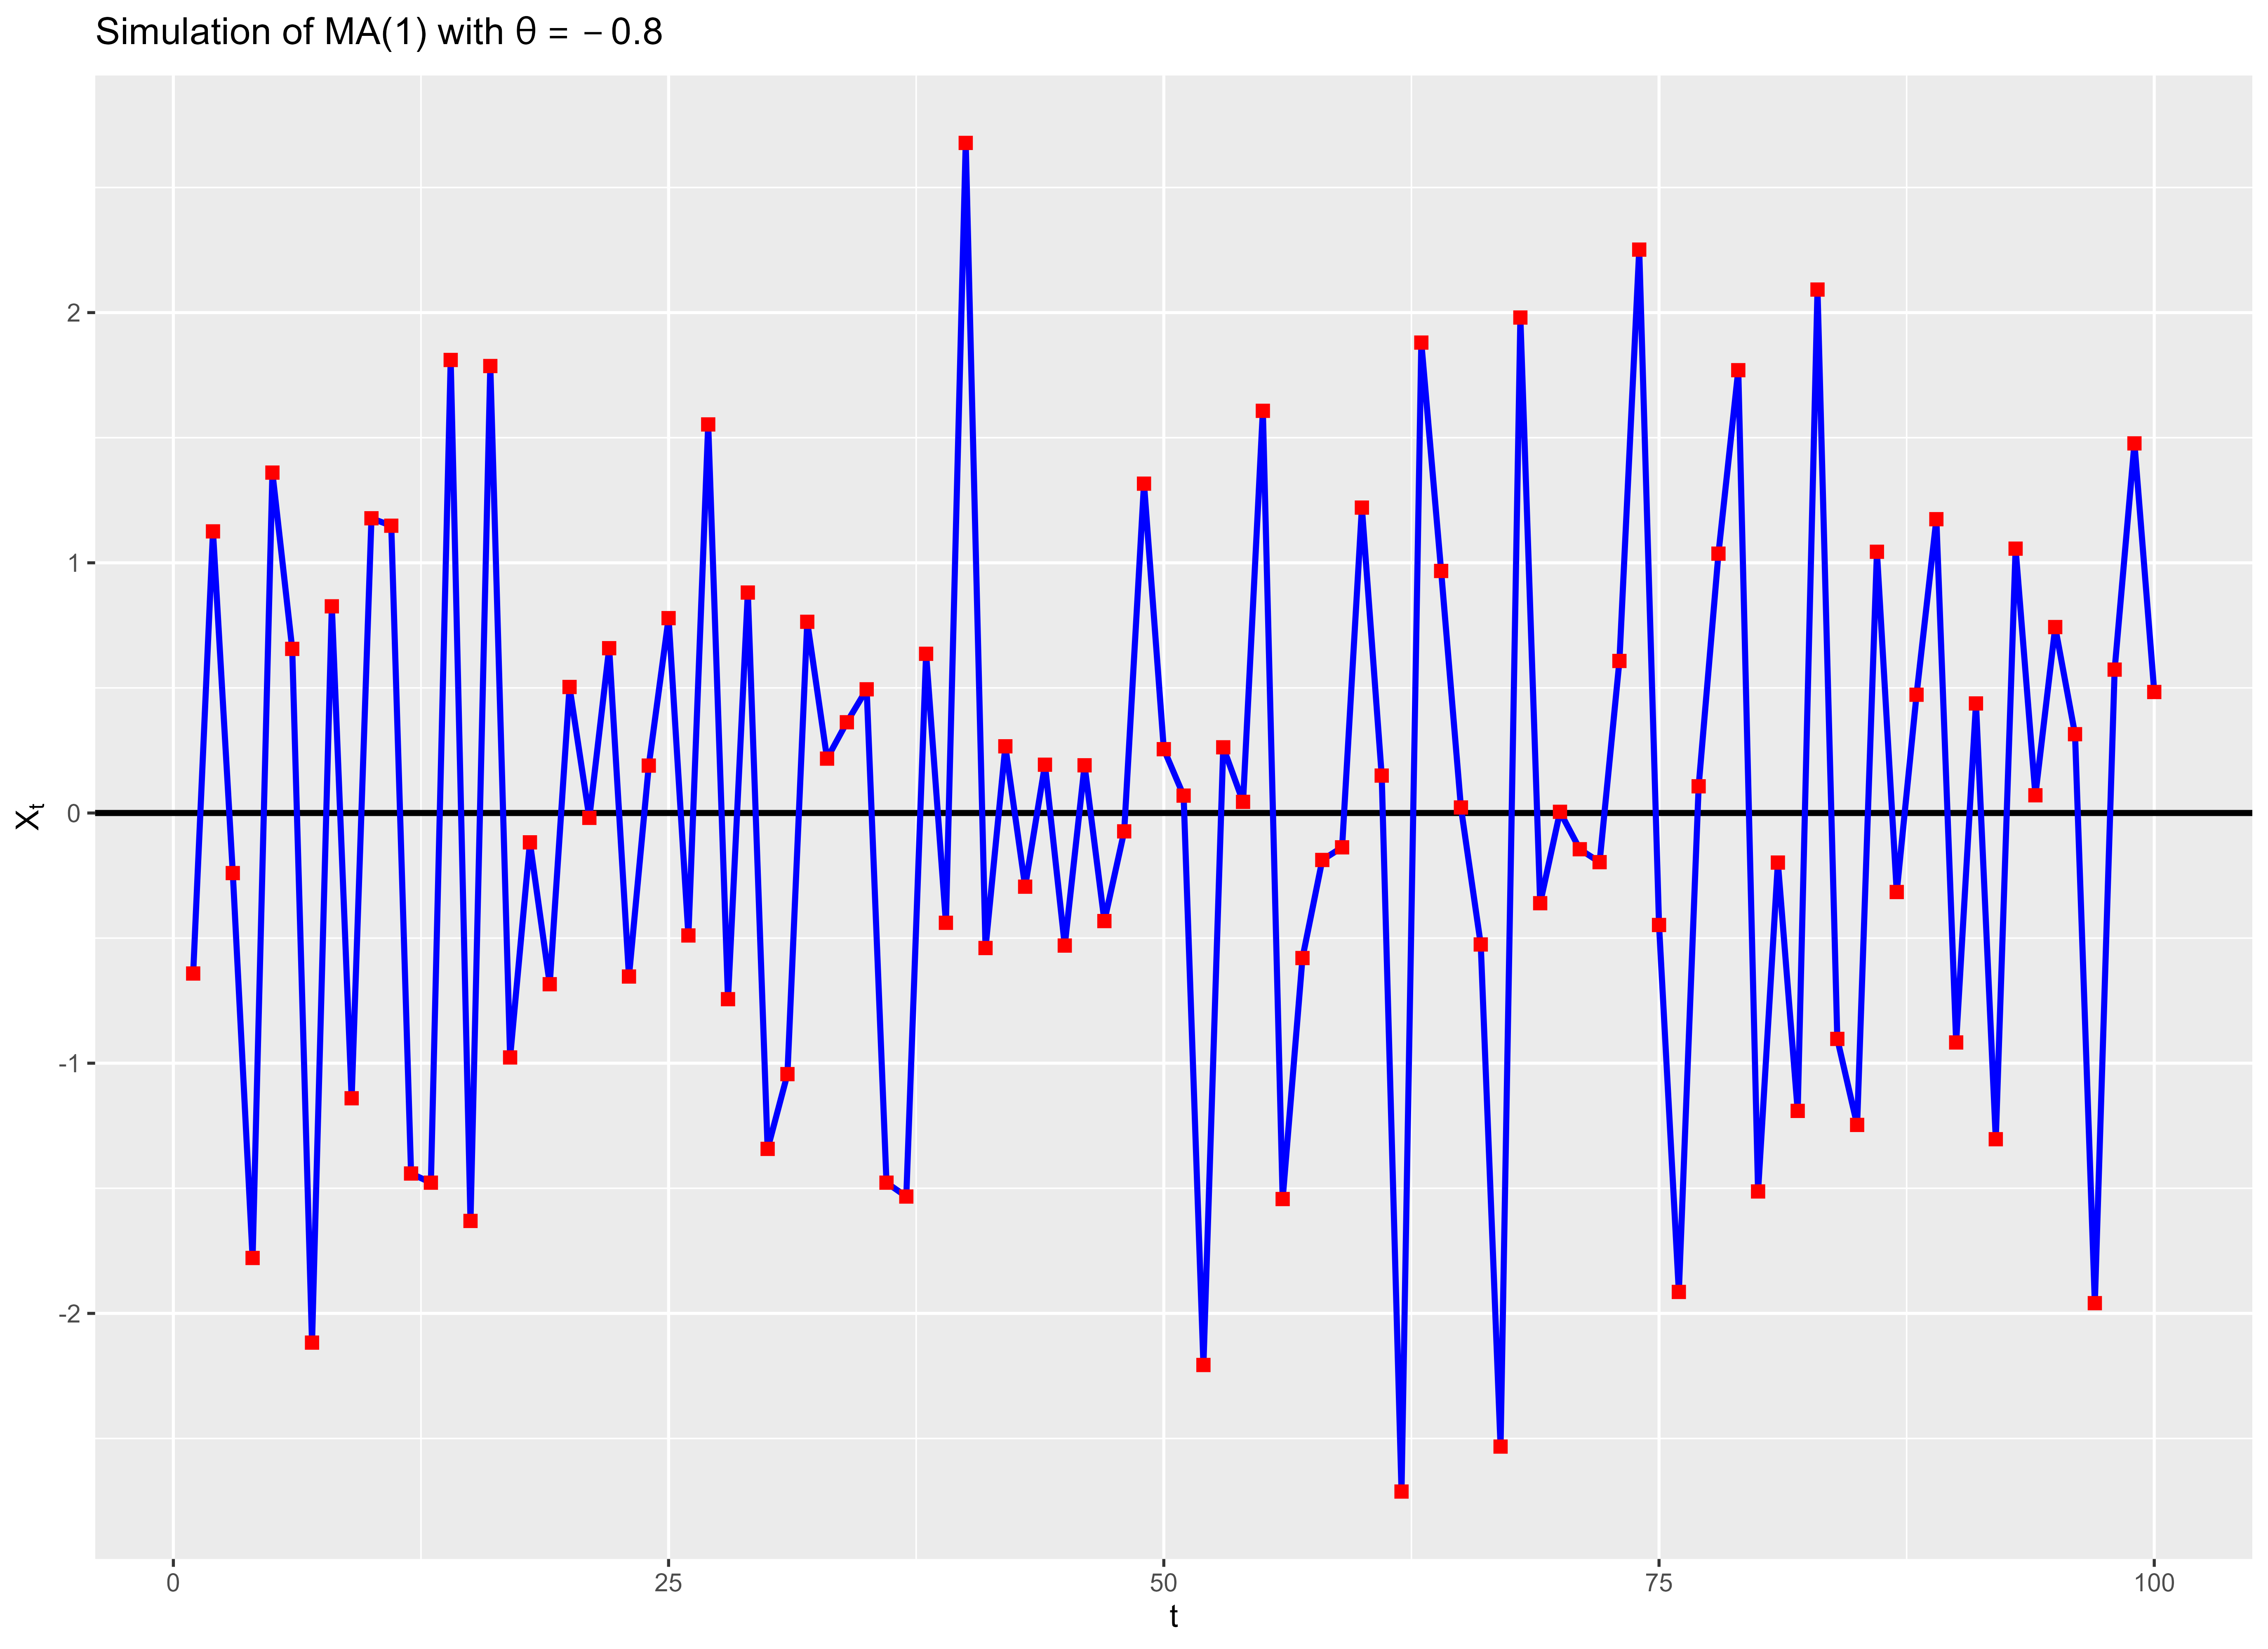
\includegraphics[scale=0.4]{figures/simulation_of_MA_1_with_theta_negative_0.8.png}
\end{figure}

$\hat{\rho}(1) = -0.3076$, theoretical $\rho(1) = -0.488$. We simulated the residuals as $X_{t} + 0.3076 X_{t-1}$ $\forall t = 3(1)100$ and $X_{t-2} + 0.3076 X_{t-1}$ $\forall t = 3(1)100$. A scatterplot of the residuals is below.

\begin{figure}[!htbp]
\centering
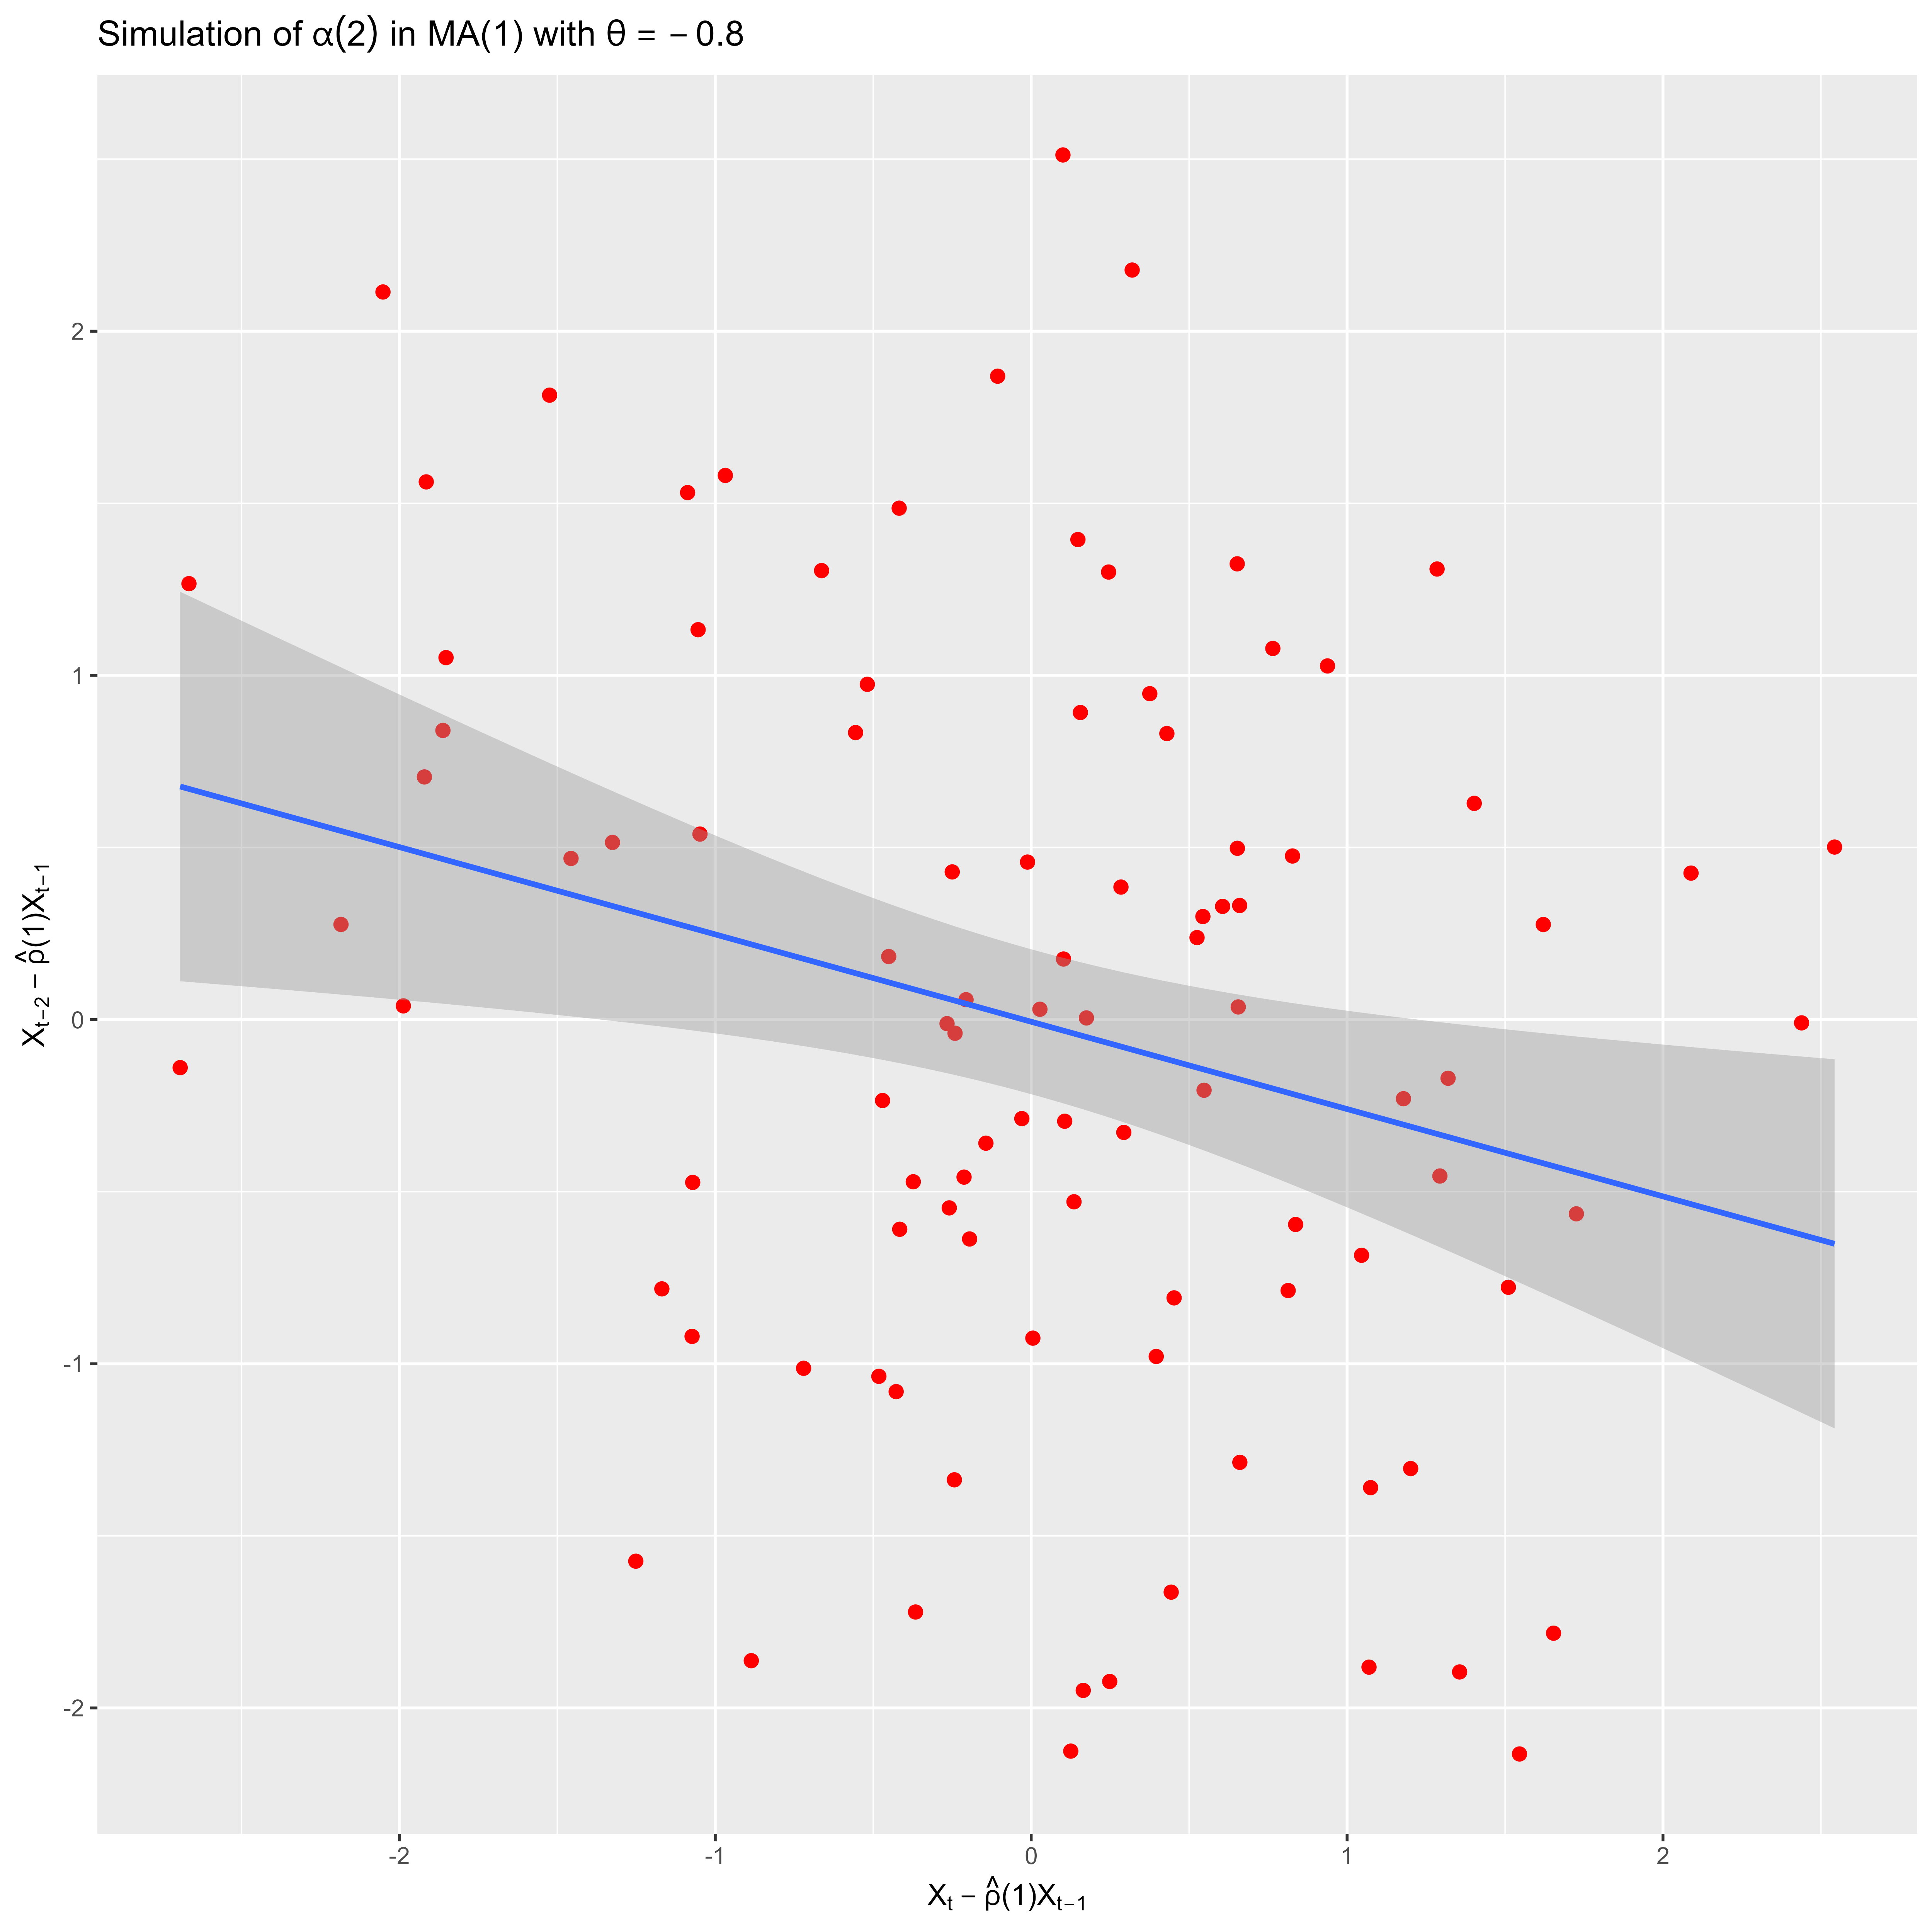
\includegraphics[scale=0.35]{figures/simulation_of_alpha_2_in_MA_1_with_theta_negative_0.8.png}
\end{figure}

\smallpencil \hspace{0.1cm} A negative linear association between the residuals is evident, sample correlation between the residuals was found to be $-0.255$ whereas theoretical correlation between the residuals \textit{i.e.} $\alpha(2)$ is $-0.312$.


\newpage

\section{Forecasting Stationary Time Series}

We now consider the problem of predicting the values $X_{n+h}, \, h > 0$, of a stationary time series with known mean $\mu$ and auto-covariance function $\gamma(\cdot)$ in terms of the values $\{X_n, \ldots, X_1\}$, up to time $n$. \\[0.25em]

$\bullet$ \textit{Conditional Expectation} and \textit{Best Linear Predictor} : The conditional expectation $$E(X_{n+h} | X_1, \ldots, X_n)$$ is the best mean square predictor of $X_{n+h}$ in terms of $X_1, \ldots, X_n$ since it minimizes the Mean Square Error $$E\left(X_{n+h} - g(X_1, \ldots, X_n) \right)^2$$ where $g(X_1, \ldots, X_n)$ is any real-valued function of the observations $X_1, \ldots, X_n$. \\[0.25em]

If we restrict $g(\cdot)$ to be a linear predictor \textit{i.e.} $g(X_1, \ldots, X_n) = a_0 + \sum \limits_{i = 1}^{n}a_i X_{n+1-i}, \, a_0, a_1, \ldots, a_n \in \mathbb{R}$, then a particular choice of $(a_0, a_1, \ldots, a_n)$ that minimizes the Mean Squared Prediction Error $$E\left(X_{n+h} - g(X_1, \ldots, X_n) \right)^2$$ is called the best linear predictor of $X_{n+h}, \, h > 0$ in terms of $X_1, \ldots, X_n$. \\ [0.25em]

\subsection{The Prediction Equations in the Time Domain}

Our goal is to find the linear combination of $1,X_n,X_{n-1}, \ldots, X_1$, that forecasts $X_{n+h}$ with minimum mean squared error. The best linear predictor in terms of $1,X_n,X_{n-1}, \ldots, X_1$ will be denoted by $P_n X_{n+h}$ and clearly has the form $$P_n X_{n+h} = a_0 + \sum \limits_{i = 1}^{n}a_i X_{n+1-i} = a_0 + a_1 X_n + a_2 X_{n-1} + \ldots + a_n X_1.$$

It remains only to determine the coefficients $a_0, a_1, \ldots, a_n \in \mathbb{R}$ by finding the values that minimize

\begin{equation}
S(a_0, a_1, \ldots, a_n) = E(X_{n+h} - a_0 - a_1 X_n - a_2 X_{n-1} - \ldots - a_n X_1)^2.
\end{equation}

Values $(a_0, a_1, \ldots, a_n)$ that minimize $S(a_0, a_1, \ldots, a_n)$ satisfy the equations
\begin{equation}
\dfrac{\partial S(a_0, a_1, \ldots, a_n)}{\partial a_j} = 0, \,\, j = 0, 1, 2, \ldots, n;
\end{equation}
equivalently
\begin{align}
&E\left[ X_{n+h} - a_0 - \sum \limits_{i = 1}^{n}a_i X_{n+1-i} \right] = 0 \label{forecastingstationarynormaleq1} \,\, \& \\[0.3em]
&E\left[ \left( X_{n+h} - a_0 - \sum \limits_{i = 1}^{n}a_i X_{n+1-i} \right) X_{n+1-j} \right] = 0, \label{forecastingstationarynormaleqrest} \,\, j = 1, 2, \ldots, n.
\end{align}

(\ref{forecastingstationarynormaleq1}) yields
\begin{align}
\mu - a_0 - \mu \cdot \sum \limits_{i = 1}^{n} a_i &= 0 \nonumber \\[0.1em]
\Rightarrow a_0 &= \mu \left( 1 - \sum \limits_{i = 1}^{n} a_i \right) \label{solutionofa0}
\end{align}

$\forall \, j = 1, 2, \ldots, n$, (\ref{forecastingstationarynormaleqrest}) yields
\begin{align}
E\left( X_{n+h} \cdot X_{n+1-j} \right) - a_0 E\left( X_{n+1-j} \right) - \sum \limits_{i = 1}^{n} a_i \cdot E\left( X_{n+1-i} \cdot X_{n+1-j} \right) &= 0 \nonumber \\[0.1em]
\Rightarrow \left[ \gamma(h+j-1) + \mu^2 - a_0 \mu \right] - \sum \limits_{i = 1}^{n} a_i \left[ \gamma(j-i) + \mu^2 \right] &= 0 \nonumber \\[0.1em]
\Rightarrow \gamma(h+j-1) - \sum \limits_{i = 1}^{n} a_i \gamma(j-i) - \mu^2 \sum \limits_{i = 1}^{n} a_i + \mu^2 - a_0 \mu &= 0 \nonumber \\[0.1em]
\Rightarrow \gamma(h+j-1) - \sum \limits_{i = 1}^{n} a_i \gamma(j-i) \, \textcolor{red}{- \mu^2 \sum \limits_{i = 1}^{n} a_i + \mu^2 - \mu^2 \left( 1 - \sum \limits_{i = 1}^{n} a_i \right)} &= 0\,\, [\text{on using }(\ref{solutionofa0})] \nonumber \\[0.1em]
\Rightarrow \gamma(h+j-1) - \sum \limits_{i = 1}^{n} a_i \gamma(j-i) &= 0 \nonumber \\[0.1em]
\Rightarrow \sum \limits_{i = 1}^{n} a_i \gamma(j-i) &= \gamma(h+j-1) \nonumber \\[0.1em]
\Rightarrow \sum \limits_{i = 1}^{n} a_i \gamma(i-j) &= \gamma(h+j-1)
\end{align}

$\therefore$ $\sum \limits_{i = 1}^{n} a_i \gamma(i-j) = \gamma(h+j-1)$ $\forall \,\, j = 1, 2, \ldots, n$. \\[0.2em]

Expanding
\begin{align*}
\text{with }j = 1, \,\, \gamma(0)a_1 + \gamma(1)a_2 + \ldots + \gamma(n-1)a_n &= \gamma(h) \\[0.1em]
\text{with }j = 2, \,\, \gamma(1)a_1 + \gamma(0)a_2 + \ldots + \gamma(n-1)a_n &= \gamma(h+1) \\[0.1em]
\vdots \hspace{1cm} \vdots \hspace{1cm} \vdots \hspace{1cm} \vdots \hspace{1cm} \vdots \hspace{1cm} \vdots \hspace{1cm} \vdots \hspace{1cm} & \vdots \hspace{1cm} \vdots \hspace{1cm} \vdots \\[0.1em]
\text{with }j = n, \,\, \gamma(n-1)a_1 + \gamma(n-2)a_2 + \ldots + \gamma(0)a_n &= \gamma(h+n-1) \\[0.1em]
\end{align*}

In matrix notation,
\begin{align}
\begin{bmatrix}
\gamma(0) & \gamma(1) & \ldots & \gamma(n-1)\\
\gamma(1) & \gamma(0) & \ldots & \gamma(n-1)\\
\vdots & \vdots & \ddots & \vdots \\
\gamma(n-1) & \gamma(n-2) & \ldots & \gamma(0)
\end{bmatrix}
\cdot
\begin{bmatrix}
a_1 \\ a_2 \\ \vdots \\ a_n
\end{bmatrix}
&=
\begin{bmatrix}
\gamma(h) \\ \gamma(h+1) \\ \vdots \\ \gamma(h+n-1)
\end{bmatrix} \label{forecastingmatrixequation} \\[0.5em]
\Rightarrow \Gamma_n \cdot \utilde{a} &= \utilde{\gamma_n(h)} \label{forecastingstationarysolution}
\end{align}

where $\Gamma_n = \left[ \gamma(i-j) \right]_{i, j = 1}^{n} = \begin{bmatrix}
\gamma(0) & \gamma(1) & \ldots & \gamma(n-1)\\
\gamma(1) & \gamma(0) & \ldots & \gamma(n-1)\\
\vdots & \vdots & \ddots & \vdots \\
\gamma(n-1) & \gamma(n-2) & \ldots & \gamma(0)
\end{bmatrix}$, \\[0.25em]
\begin{center}
$\utilde{a} = \begin{bmatrix}
a_1 \\ a_2 \\ \vdots \\ a_n
\end{bmatrix}$ and $\utilde{\gamma_n(h)} = \begin{bmatrix}
\gamma(h) \\ \gamma(h+1) \\ \vdots \\ \gamma(h+n-1)
\end{bmatrix}$.
\end{center}

Hence,
\begin{equation}\label{forecastingstationarypredictionequation}
P_n X_{n+h} = \mu + \sum \limits_{i = 1}^{n} a_i \cdot \left( X_{n+1-i} - \mu \right)
\end{equation}
where $\utilde{a} = \left( a_1, a_2, \ldots, a_n \right)'$ satisfies (\ref{forecastingstationarysolution}). \\[0.1em]

From (\ref{forecastingstationarypredictionequation}), the expected prediction error
\begin{align*}
E\left[ X_{n+h} - P_n X_{n+h} \right] &= E\left[ X_{n+h} - \mu - \sum \limits_{i = 1}^{n} a_i \cdot \left( X_{n+1-i} - \mu \right) \right] \\[0.1em]
&= E\left[ X_{n+h} - \mu \right] - \left[ \sum \limits_{i = 1}^{n} a_i \cdot E\left( X_{n+1-i} - \mu \right) \right] \\[0.1em]
&= 0
\end{align*}
and the mean square prediction error
\begin{align*}
&E\left[ X_{n+h} - P_n X_{n+h} \right]^2 \\[0.1em]
=\,\, &E\left[ X_{n+h} - \mu - \sum \limits_{i = 1}^{n} a_i \cdot \left( X_{n+1-i} - \mu \right) \right]^2 \\[0.1em]
=\,\, &E\left[ \left( X_{n+h} - \mu \right)^2 \right] - 2 \sum \limits_{i = 1}^{n} a_i \cdot E\left[ \left( X_{n+h} - \mu \right) \cdot \left( X_{n+1-i} - \mu \right)\right] + E\left[\sum \limits_{i = 1}^{n} a_i \cdot \left( X_{n+1-i} - \mu \right) \right]^2 \\[0.1em]
=\,\, &E\left[ \left( X_{n+h} - \mu \right)^2 \right] - 2 \sum \limits_{i = 1}^{n} a_i \cdot E\left[ \left( X_{n+h} - \mu \right) \cdot \left( X_{n+1-i} - \mu \right)\right] + E\left[\sum \limits_{i = 1}^{n} \sum \limits_{j = 1}^{n} a_i \cdot \left( X_{n+1-i} - \mu \right) \cdot \left( X_{n+1-j} - \mu \right) \cdot a_j \right] \\[0.1em]
=\,\, &\gamma(0) - 2 \sum \limits_{i = 1}^{n} a_i \cdot \gamma(h+i-1) + \sum \limits_{i = 1}^{n} \sum \limits_{j = 1}^{n} a_i \cdot \gamma(j-i) \cdot a_j \\[0.1em]
=\,\, &\gamma(0) - 2 \utilde{a}' \cdot \utilde{\gamma_n(h)} + \utilde{a}' \cdot \underbrace{\Gamma_n \cdot \utilde{a}}_{\utilde{\gamma_n(h)}} \,\,\,\, [\text{Recall } (\ref{forecastingstationarysolution})] \\[0.1em]
=\,\, &\gamma(0) - 2 \utilde{a}' \cdot \utilde{\gamma_n(h)} + \utilde{a}' \cdot \utilde{\gamma_n(h)} \\[0.1em]
=\,\, &\gamma(0) - \utilde{a}' \cdot \utilde{\gamma_n(h)}.
\end{align*}

\subsection{Equations for the One-Step Predictors, $h = 1$}

$\bullet$ Denote $\utilde{\gamma_n} := \utilde{\gamma_n (1)}$. \\[0.1em]

The best linear predictor $P_nX_{n+1}$ of $X_{n+1}$ in terms of $X_1, X_2, \ldots, X_n$ is
\begin{equation}\label{onesteppredictionequation}
P_nX_{n+1} = \sum \limits_{i = 1}^{n} \phi_{ni} X_{n+1-i}, \qquad n = 1, 2, \ldots,
\end{equation}
where $\utilde{\phi_n} := \left( \phi_{n1}, \phi_{n2}, \ldots, \phi_{nn} \right)'$ is any solution (unique if $\Gamma_n$ is non-singular) of 
\begin{equation}\label{onesteppredictionmatrixequation}
\Gamma_n \cdot \utilde{\phi_n} = \utilde{\gamma_n}
\end{equation} 
where $\utilde{\gamma_n} := \left(\gamma(1), \gamma(2), \ldots, \gamma(n) \right)'$ and $\Gamma_n = \left[ \gamma(i-j) \right]_{i, j = 1}^{n}$. The corresponding mean squared error is 
\begin{equation}\label{onesteppredictionequationMSE}
v_n := E\left[ X_{n+1} - P_n X_{n+1} \right]^2 = \gamma(0) - \utilde{\phi_n}' \utilde{\gamma_n}, \qquad n \geq 1.
\end{equation}
and clearly $v_0 = \gamma(0)$.

\begin{proposition}\label{sufficientconditionforinvertibilityofGamma}
(A useful sufficient condition) If $\gamma(0) > 0$ and $\gamma(h) \rightarrow 0$ as $h \rightarrow \infty$ then the covariance matrix $\Gamma_n = \left[ \gamma(i-j) \right]_{i, j = 1}^{n}$ of $\left( X_1, X_2, \ldots, X_n \right)'$ is non-singular for every $n$.
\end{proposition}

\begin{corollary}
Under the conditions of Proposition (\ref{sufficientconditionforinvertibilityofGamma}), the best linear predictor $P_nX_{n+1}$ of $X_{n+1}$ in terms of $X_1, X_2, \ldots, X_n$ is
$$P_nX_{n+1} = \sum \limits_{i = 1}^{n} \phi_{ni} X_{n+1-i}, \qquad n = 1, 2, \ldots,$$
where $\utilde{\phi_n} := \left( \phi_{n1}, \phi_{n2}, \ldots, \phi_{nn} \right)' = \Gamma_n^{-1} \utilde{\gamma_n}$, $\utilde{\gamma_n} := \left(\gamma(1), \gamma(2), \ldots, \gamma(n) \right)'$ and $\Gamma_n = \left[ \gamma(i-j) \right]_{i, j = 1}^{n}$ and the corresponding mean squared error is $v_n = \gamma(0) - \utilde{\gamma_n}' \Gamma_n^{-1} \utilde{\gamma_n} $.
\end{corollary}

\subsection{Equations for the $h-$Step Predictors, $h \geq 1$}

The best linear predictor $P_nX_{n+h}$ of $X_{n+h}$ in terms of $X_1, X_2, \ldots, X_n$ is
\begin{equation}\label{hsteppredictionequation}
P_nX_{n+h} = \sum \limits_{i = 1}^{n} \phi_{ni}^{(h)} X_{n+1-i} = \phi_{n1}^{(h)} X_{n} + \phi_{n2}^{(h)} X_{n-1} + \ldots + \phi_{nn}^{(h)} X_{1}, \qquad n = 1, 2, \ldots,
\end{equation}
where $\utilde{\phi_n^{(h)}} := \left( \phi_{n1}^{(h)}, \phi_{n2}^{(h)}, \ldots, \phi_{nn}^{(h)} \right)'$ is any solution (unique if $\Gamma_n$ is non-singular) of 
\begin{equation}\label{hsteppredictionmatrixequation}
\Gamma_n \cdot \utilde{\phi_n^{(h)}} = \utilde{\gamma_n (h)}
\end{equation} 
where $\utilde{\gamma_n (h)} := \left(\gamma(h), \gamma(h+1), \ldots, \gamma(n+h-1) \right)'$ and $\Gamma_n = \left[ \gamma(i-j) \right]_{i, j = 1}^{n}$. The corresponding mean squared error is 
\begin{equation}\label{hsteppredictionequationMSE}
v_n := E\left[ X_{n+h} - P_n X_{n+h} \right]^2 = \gamma(0) - \utilde{\phi_n^{(h)}}' \utilde{\gamma_n (h)}.
\end{equation}

\subsection{One-step Prediction of a stationary AR(1) Process}

Consider a stationary AR$(1)$ process $\{X_t\}$ defined by the equation (\ref{ar1}) with $|\alpha| < 1$ and \\ $Z_t \overset{iid}{\sim} \text{ WN }(0, \sigma^2)$. Recall that, $E(X_t) = 0, \, t = 0, \pm 1, \pm 2, \ldots$. \\[0.1em]

Following (\ref{solutionofa0}) and (\ref{forecastingstationarysolution}), the best linear predictor of $X_{n+1}$ in terms of $X_n, X_{n-1}, \ldots, X_1$ is
$$P_n X_{n+1} = \utilde{a}'\utilde{X_n}$$
where $\utilde{X_n} = (X_n, X_{n-1}, \ldots, X_1)'$. \\[0.1em]

Recall that for an AR$(1)$ process, $\gamma(h) = \dfrac{\sigma^2\alpha^{|h|}}{1-\alpha^2}, \, h = 0, \pm 1, \pm 2, \ldots$. Then (\ref{forecastingstationarysolution}) yields
\begin{align*}
\begin{bmatrix}
1 & \alpha & \ldots & \alpha^{n-1}\\
\alpha & 1 & \ldots & \alpha^{n-1}\\
\vdots & \vdots & \ddots & \vdots \\
\alpha^{n-1} & \alpha^{n-2} & \ldots & 1
\end{bmatrix}
\cdot
\begin{bmatrix}
a_1 \\ a_2 \\ \vdots \\ a_n
\end{bmatrix}
&=
\begin{bmatrix}
\alpha \\ \alpha^{2} \\ \vdots \\ \alpha^{n}
\end{bmatrix} \,\, \text{after factoring out } \dfrac{\sigma^2}{1 - \alpha^2}
\end{align*}
and leads to an obvious solution $\utilde{a} = (a_1, a_2, \ldots, a_n)' = (\alpha, 0, \ldots, 0)'$. \\[0.1em]

Hence the best linear predictor of $X_{n+1}$ in terms of $X_n, X_{n-1}, \ldots, X_1$ is $$P_n X_{n+1} = \utilde{a}'\utilde{X_n} = \alpha \cdot X_n$$
with mean square prediction error
\begin{align*}
&E\left[ X_{n+h} - P_n X_{n+1} \right]^2 \\[0.3em]
=\,\, &\gamma(0) - \utilde{a}' \cdot \utilde{\gamma_n(1)} \\[0.3em]
=\,\, &\dfrac{\sigma^2}{1 - \alpha^2} - \alpha \cdot \gamma(1) \\[0.3em]
=\,\, &\dfrac{\sigma^2}{1 - \alpha^2} - \alpha \cdot \dfrac{\sigma^2 \alpha}{1 - \alpha^2} \\[0.3em]
=\,\, &\dfrac{\sigma^2}{1 - \alpha^2} (1-\alpha^2) \\[0.3em]
=\,\, &\sigma^2.
\end{align*}

\subsection{Recursive Methods for Computing Best Linear Predictors}

Here we establish two recursive algorithms for determining the one-step predictors $P_nX_{n+1}, \, n \geq 1$, defined by (\ref{onesteppredictionequation}) and show they can be used also to compute the $h-$step predictors $P_nX_{n+h}, \, n \geq 1$, defined by (\ref{hsteppredictionequation}). Recursive prediction is of great practical importance since direct computation of $P_nX_{n+h}$ from (\ref{hsteppredictionequation}) and (\ref{hsteppredictionmatrixequation}) requires, for large $n$, the solution of a large system of linear equations. Moreover, each time the number of observations is increased, the whole procedure must be repeated. The algorithms to be described in this section however allow us to compute best predictors without having to perform any matrix inversions. Furthermore they utilize the predictors based on $n$ observations to compute those based on $n+1$ observations, $n = 1, 2, \ldots$. Prediction algorithms that utilize this idea are said to be \textbf{recursive}.

\subsubsection{The Durbin-Levinson Algorithm}

The algorithm specified in the following proposition, known as the Durbin-Levinson algorithm, is a recursive scheme for computing $\utilde{\phi_n} := \left( \phi_{n1}, \phi_{n2}, \ldots, \phi_{nn} \right)'$ and $v_n$ for $n = 1, 2, \ldots$.

\begin{proposition}
(The Durbin-Levinson Algorithm) If $\{X_t\}$ is a zero mean stationary process with autocovariance function $\gamma(\cdot)$ such that $\gamma(0) > 0$ and $\gamma(h) \rightarrow 0$ as $h \rightarrow \infty$, then the coefficients $\phi_{ni}$ and mean squared errors $v_n$ as defined by (\ref{onesteppredictionequation}) and (\ref{onesteppredictionequationMSE}) respectively satisfy $\phi_{11} = \gamma(1) / \gamma(0)$, $v_0 = \gamma(0)$,
\begin{equation}\label{DLphinnupdate}
\phi_{nn} = \left[ \gamma(n) - \sum \limits_{j = 1}^{n-1} \phi_{n-1, j} \cdot \gamma(n-j) \right] v_{n-1}^{-1},
\end{equation}

\begin{equation}\label{DLphivectorupdate}
\begin{bmatrix}
\phi_{n1} \\ \vdots \\ \phi_{n, n-1} 
\end{bmatrix}
= 
\begin{bmatrix}
\phi_{n-1, 1} \\ \vdots \\ \phi_{n-1, n-1} 
\end{bmatrix}
- \phi_{nn} \cdot
\begin{bmatrix}
\phi_{n-1, n-1} \\ \vdots \\ \phi_{n-1, 1} 
\end{bmatrix}
\end{equation}

and

\begin{equation}\label{DLMSEupdate}
v_n = v_{n-1} \left[ 1 - \phi_{nn}^2 \right].
\end{equation}
\end{proposition}

\bcattention \hspace{0.1cm} \textbf{Partial Autocorrelation Function} : Recall the partial autocorrelation function, definition (\ref{PACFdefinition1}). Dividing both sides of (\ref{forecastingmatrixequation}, $h = 1$) by $\gamma(0)$ we can write
\begin{equation}\label{forecastingmatrixequationinrho}
\begin{bmatrix}
\rho(0) & \rho(1) & \rho(2) & \ldots & \rho(k-1)\\
\rho(1) & \rho(0) & \rho(1) & \ldots & \rho(k-1)\\
\vdots & \vdots & \vdots & \ddots & \vdots \\
\rho(k-1) & \rho(k-2) & \rho(k-3) & \ldots & \rho(0)
\end{bmatrix}
\cdot
\begin{bmatrix}
\phi_{k1} \\ \phi_{k2} \\ \vdots \\ \phi_{kk}
\end{bmatrix}
=
\begin{bmatrix}
\rho(1) \\ \rho(2) \\ \vdots \\ \rho(k)
\end{bmatrix} , \qquad k \geq 1.
\end{equation}

\begin{definition}\label{PACFdenfinition2}
The partial autocorrelation function $\alpha(k)$ of $\{X_t\}$ at lag $k$ is
$$\alpha(k) = \phi_{kk}$$
where $\phi_{kk}$ is uniquely determined by (\ref{forecastingmatrixequationinrho}).
\end{definition}

Equation (\ref{DLMSEupdate}) shows the relation between $\alpha(n)$ and the reduction in the one-step mean squared error as the number of predictors is increased from $n-1$ to $n$. \\[0.2em]

As a continuation of Section \ref{PACFofARp}, now we try to obtain $\alpha(k)$, $k = 1, 2$ for an AR$(2)$ process by using definition \ref{PACFdenfinition2}. Consider a stationary AR$(2)$ process defined by (\ref{ar2}). From definition \ref{PACFdefinition1}, 
$$\alpha(1) = \rho(1).$$
From (\ref{yulewalker2}), with $h = 1$ we have
\begin{align*}
\rho(1) &= \alpha_1 \rho(0) + \alpha_2 \rho(-1) \\[0.2em]
\Rightarrow \rho(1) &= \alpha_1 + \alpha_2 \rho(1) \\[0.2em]
\Rightarrow \rho(1) &= \dfrac{\alpha_1}{1 - \alpha_2}.
\end{align*}

$$\therefore \, \alpha(1) = \dfrac{\alpha_1}{1 - \alpha_2}.$$

Now, $\alpha(2) = \phi_{22}$. From (\ref{DLphinnupdate}),
$$\phi_{22} = \left[ \gamma(2) - \phi_{1, 1} \cdot \gamma(1) \right] v_{1}^{-1}.$$

From (\ref{DLMSEupdate}), $v_1 = v_{0} \left[ 1 - \phi_{11}^2 \right]$. Recall $\phi_{11} = \alpha(1)$, from definition \ref{PACFdenfinition2}. Also $v_0 = \gamma(0)$. Thus
\begin{align*}
\phi_{22} &= \dfrac{\gamma(2) - \phi_{11} \cdot \gamma(1)}{\gamma(0) \left[ 1 - \phi_{11}^2 \right]} \\[0.2em]
&= \dfrac{\rho(2) - \rho(1)^2}{1 - \rho(1)^2}
\end{align*}

From (\ref{yulewalker2}), with $h = 2$ we have $\rho(2) = \alpha_1 \rho(1) + \alpha_2 \rho(0) = \alpha_1 \rho(1) + \alpha_2$.

\begin{align*}
\therefore \phi_{22} &= \dfrac{\alpha_1 \rho(1) + \alpha_2 - \rho(1)^2}{1 - \rho(1)^2} \\[0.2em]
&= \dfrac{\alpha_1 \cdot \left( \dfrac{\alpha_1}{1 - \alpha_2} \right) + \alpha_2 - \left( \dfrac{\alpha_1}{1 - \alpha_2} \right)^2}{1 - \left( \dfrac{\alpha_1}{1 - \alpha_2} \right)^2} \\[0.2em]
&= \dfrac{\left( \dfrac{\alpha_1^2}{1 - \alpha_2} \right)\left( 1 -  \dfrac{1}{1 - \alpha_2} \right) + \alpha_2}{1 - \left( \dfrac{\alpha_1}{1 - \alpha_2} \right)^2} \\[0.2em]
&= \dfrac{\alpha_2 - \alpha_2 \left( \dfrac{\alpha_1}{1 - \alpha_2} \right)^2}{1 - \left( \dfrac{\alpha_1}{1 - \alpha_2} \right)^2} \\[0.2em]
&= \alpha_2
\end{align*}

$$\therefore \, \alpha(2) = \alpha_2.$$

\subsubsection{The Innovations Algorithm}

\section{Estimation for ARMA Models}

The determination of an appropriate ARMA$(p, q)$ model to represent an 
observed stationary time series involves a number of inter-related problems. These include the choice of $p$ and $q$ (order selection), and estimation of the remaining parameters, \textit{i.e.} the mean, the coefficients $\{\phi_i; i = 1, 2, \ldots, p\}$, $\{\theta_j; j = 1, 2, \ldots, q\}$ and the white noise variance $\sigma^2$, for given values of $p$ and $q$. This section is devoted to the most straightforward part of the modelling procedure, namely the estimation, for fixed values of $p$ and $q$, of the parameters $\boldsymbol{\phi} = (\phi_1, \phi_2, \ldots, \phi_p)'$, $\boldsymbol{\theta} = (\theta_1, \theta_2, \ldots, \theta_q)'$ and $\sigma^2$. It will be \textit{assumed} throughout that the data has been adjusted by subtraction of the mean, so our problem becomes that of fitting a zero-mean ARMA model to the adjusted data $x_1, \ldots, x_n$.

\subsection{Parameter Estimation for Autoregressive Processes}

\subsubsection{Yule-Walker Estimates}

Let $\{X_t\}$ be a zero-mean\footnote{Any non-zero mean $\mu$ is estimated by sample mean, \textit{i.e.} $\hat{\mu} = \overline{X}$. Then we subtract $\overline{X}$ to get a zero-mean time series.} causal AR$(p)$ process defined by
\begin{equation}\label{arp_phi}
X_t - \phi_1 X_{t-1} - \ldots - \phi_p X_{t-p} = Z_t, \qquad \{Z_t\} \overset{iid}{\sim} WN(0, \sigma^2).
\end{equation}

Our aim is to find estimators of the coefficient vector $\boldsymbol{\phi} = (\phi_1, \phi_2, \ldots, \phi_p)'$ and the white noise variance $\sigma^2$ based on the observations $X_1, \ldots, X_n$. \\[0.1em]

The causality assumption allows us to write $X_t$, in the form
\begin{equation}\label{arp_causality}
X_t = \sum \limits_{j = 0}^{\infty} \psi_j Z_{t-j}, \,\, \forall t
\end{equation}

Multiplying both sides of (\ref{arp_phi}) by $X_{t-j}, \, j = 0, 1, \ldots, p$, we obtain the following set of equations.

\begin{align*}
X_t \cdot X_t - \phi_1 X_t \cdot X_{t-1} - \ldots - \phi_p X_t \cdot X_{t-p} &= X_t \cdot Z_t = Z_t \cdot \sum \limits_{j = 0}^{\infty} \psi_j Z_{t-j} \\[0.2em]
X_{t-1} \cdot X_t - \phi_1 X_{t-1} \cdot X_{t-1} - \ldots - \phi_p X_{t-1} \cdot X_{t-p} &= X_{t-1} \cdot Z_t = Z_t \cdot \sum \limits_{j = 0}^{\infty} \psi_j Z_{t-1-j} \\[0.2em]
\vdots \hspace{1cm} \vdots \hspace{1cm} \vdots \hspace{1cm} \vdots \hspace{1cm} \vdots \hspace{1cm} \vdots \hspace{1cm} \vdots \hspace{1cm} \vdots & \hspace{1cm} \vdots  \hspace{1cm} \vdots \hspace{1cm} \vdots \hspace{1cm} \vdots \\[0.2em]
X_{t-p} \cdot X_t - \phi_1 X_{t-p} \cdot X_{t-1} - \ldots - \phi_p X_{t-p} \cdot X_{t-p} &= X_{t-p} \cdot Z_t = Z_t \cdot \sum \limits_{j = 0}^{\infty} \psi_j Z_{t-p-j}
\end{align*}

Taking expectations and using (\ref{arp_causality}) to evaluate the right-hand sides,  we get,
\begin{align*}
\gamma(0) - \phi_1 \gamma(1) - \ldots - \phi_p \gamma(p) &= \sigma^2 \\[0.2em]
\gamma(1) - \phi_1 \gamma(0) - \ldots - \phi_p \gamma(p-1) &= 0 \\[0.2em]
\vdots \hspace{1cm} \vdots \hspace{1cm} \vdots \hspace{1cm} \vdots \hspace{1cm} \vdots & \hspace{0.5cm} \vdots \\[0.2em]
\gamma(p) - \phi_1 \gamma(p-1) - \ldots - \phi_p \gamma(0) &= 0
\end{align*}

Rearranging,
\begin{align*}
\sigma^2 = \gamma(0) - \phi_1 \gamma(1) - \ldots - \phi_p \gamma(p)
\end{align*}
\begin{center}and\end{center}
\begin{align*}
\phi_1 \gamma(0) + \ldots + \phi_p \gamma(p-1) &= \gamma(1) \\[0.2em]
\vdots \hspace{1cm} \vdots \hspace{1cm} \vdots \hspace{1cm} \vdots & \hspace{1cm} \vdots \\[0.2em]
\phi_1 \gamma(p-1) + \ldots + \phi_p \gamma(0) &= \gamma(p)
\end{align*}

Finally we obtain a set of Yule-Walker equations as follows.
\begin{align}
\sigma^2 = \gamma(0) - \utilde{\phi}' \cdot \utilde{\gamma_p},
\end{align}
\begin{center}and\end{center}
\begin{align}\label{AR_p_phi_Yule_Walker}
\Gamma_p \cdot \utilde{\phi} = \utilde{\gamma_p}.
\end{align}

where $\Gamma_p = \left[ \gamma(i - j) \right]_{i, j = 1}^{p}$ and $\utilde{\gamma_p} = \left( \gamma(1), \gamma(2), \ldots, \gamma(p) \right)'$. \\[0.1em]

If we replace the covariances $\gamma(j), \, j = 0, 1, 2, \ldots, p$ by corresponding sample covariances, we obtain Yule-Walker estimates $\utilde{\hat{\phi}}$ and $\hat{\sigma}^2$ given by equations
\begin{align}\label{ARestimationGammahat}
\widehat{\Gamma}_p \cdot \utilde{\hat{\phi}} = \hat{\gamma_p}
\end{align}
\begin{center}and\end{center}
\begin{align}
\hat{\sigma}^2 = \hat{\gamma}(0) - \utilde{\hat{\phi}}' \cdot \utilde{\hat{\gamma_p}}
\end{align}
where $\widehat{\Gamma}_p = \left[ \hat{\gamma}(i - j) \right]_{i, j = 1}^{p}$ and $\utilde{\hat{\gamma_p}} = \left( \hat{\gamma}(1), \hat{\gamma}(2), \ldots, \hat{\gamma}(p) \right)'$. \\[0.1em]

If $\hat{\gamma}(0) > 0$, $\widehat{\Gamma}_p$ is non-singular. Dividing each side of (\ref{ARestimationGammahat}) by $\hat{\gamma}(0)$ we get Yule-Walker estimates
\begin{align}
\utilde{\hat{\phi}} = \widehat{R_p}^{-1} \cdot \utilde{\hat{\rho_p}}
\end{align}
\begin{center}and\end{center}
\begin{align}
\hat{\sigma}^2 = \hat{\gamma}(0) \left[ 1 - \utilde{\hat{\rho_p}}' \widehat{R_p}^{-1} \utilde{\hat{\rho_p}} \right]
\end{align}
where $\utilde{\hat{\rho_p}} = \left( \hat{\rho}(1), \hat{\rho}(2), \ldots, \hat{\rho}(p) \right)' = \hat{\gamma_p} / \hat{\gamma}(0)$. Note that, the Yule-Walker estimates are also Method of Moments estimates.

\subsubsection{Large Sample Properties of Yule-Walker Estimates}

If $\{X_t\}$ is the causal AR$(p)$ process (\ref{arp_phi}) with $\{Z_t\}\sim \text{IID}(0,\sigma^2)$, and if $\hat{\boldsymbol{\phi}}_m = (\hat{\phi}_{m1},\ldots,\hat{\phi}_{mm})' = \hat{\mathbf{R}}_m^{-1}\hat{\boldsymbol{\rho}}_m$, $m>p$, then
\[
n^{1/2}(\hat{\boldsymbol{\phi}}_m - \boldsymbol{\phi}_m) \; \overset{d}{\rightarrow}\; N(0,\sigma^2 \Gamma_m^{-1}),
\]
where $\boldsymbol{\phi}_m$ is the coefficient vector of the best linear predictor $\boldsymbol{\phi}_m' \mathbf{X}_m$ of $X_{m+1}$ based on 
$\mathbf{X}_m = (X_m,\ldots,X_1)'$, i.e. $\boldsymbol{\phi}_m = \mathbf{R}_m^{-1}\boldsymbol{\rho}_m$. In particular for $m>p$,
\[
n^{1/2}\hat{\phi}_{mm} \;\overset{d}{\rightarrow}\; N(0,1).
\]

\subsubsection{An Example of Yule-Walker Estimates}

\fcChick[scale = 0.4, draw = yellow, line width = 1.5] We simulate\footnote{R Program : \href{https://raw.githubusercontent.com/sakunisgithub/Time_Series_Analysis/refs/heads/master/R_Programs/Yule_Walker_estimates_of_an_AR_2_process.R}{Yule\_Walker\_estimates\_of\_an\_AR\_2\_process.R}} $n = 150$ observations from an AR$(2)$ process given by $X_t = 1.5 X_{t-1} - 0.75X_{t-2} + Z_t$ with $Z_t \overset{iid}{\sim} WN(0, \sigma^2 = 1)$. The sample autocovariances are $\hat{\gamma}(0) = 9.000191$, $\hat{\gamma}(1) = 7.860891$, $\hat{\gamma}(2) = 5.320132$. We obtain the Yule-Walker estimates as follows :
\begin{align*}
\utilde{\hat{\phi}}
=
\begin{pmatrix}
\hat{\phi}_1 \\ \hat{\phi}_2
\end{pmatrix}
&= \widehat{\Gamma}_2^{-1} \cdot \hat{\gamma}_2 \\[0.2em]
&= \begin{pmatrix}
\hat{\gamma}(0) & \hat{\gamma}(1) \\
\hat{\gamma}(1) & \hat{\gamma}(0)
\end{pmatrix}^{-1}
\cdot
\begin{pmatrix}
\hat{\gamma}(0) \\ \hat{\gamma}(1)
\end{pmatrix} \\[0.2em]
&= \begin{pmatrix}
1.5059237 \\ -0.7241813
\end{pmatrix}
\approx \begin{pmatrix}
1.51\\ -0.72
\end{pmatrix};
\end{align*}

and

\begin{align*}
\hat{\sigma}^2 &= \hat{\gamma}(0) - \begin{pmatrix}
\hat{\phi}_1 & \hat{\phi}_2
\end{pmatrix} \cdot \begin{pmatrix}
\hat{\gamma}(0) \\ \hat{\gamma}(1)
\end{pmatrix} \\[0.2em]
&= 1.015029 \approx 1.02.
\end{align*}

So the fitted model is
$$X_t = 1.51X_{t-1} - 0.72X_{t-2} + Z_t$$
with estimated noise variance $1.02$.


\subsubsection{Maximum Likelihood Estimation for AR(1) Process}

The method of moments is unsatisfactory for many models, so we consider other methods of estimation. At this point, we introduce a possibly non-zero mean $\mu$, into our stationary models and treat it as another parameter to be estimated. \\[0.1em]

Let us focus on the \textbf{causal} AR(1) case where

\begin{equation}\label{ar1meanmu}
X_t -  \mu = \phi( X_{t-1} - \mu) + Z_t
\end{equation}

where $|\phi| < 1$ and $Z_t \overset{iid}{\sim} N(0, \sigma^2)$. Given data $x_1, x_2, \ldots, x_n$, we seek likelihood

\begin{equation}
L(\mu, \phi, \sigma^2) = f_{\utilde{X}} (x_1, x_2, \ldots, x_n) = \prod \limits_{t = 1}^{n} f(x_t | x_{t-1}, \ldots, x_1),
\end{equation}

where, to ease the notation, we have dropped the parameters in the densities $f(\cdot | \cdot)$. In the case of an AR(1), we may write the likelihood as

\begin{equation}
L(\mu, \phi, \sigma^2) = f(x_1) \cdot f(x_2 | x_1) \cdot f(x_3 | x_2) \cdot \ldots \cdot f(x_n | x_{n-1}).
\end{equation}

From (\ref{ar1meanmu}), as $Z_t \sim N(0, \sigma^2)$, $x_t | x_{t-1} \sim N(\mu + \phi(x_{t-1} - \mu), \sigma^2)$. Thus

\begin{equation}
\forall \,\, t \geq 2, \qquad f(x_t | x_{t-1}) = f_Z\left[ (x_t - \mu) - \phi(x_{t-1} - \mu) \right]
\end{equation}

where $f_Z(\cdot)$ is the density of $Z_t$; i.e., the normal density with mean zero and variance $\sigma^2$. We may write the likelihood as

\begin{equation}
L(\mu, \phi, \sigma^2) = f(x_1) \cdot \prod \limits_{t = 2}^{n} f_Z\left[ (x_t - \mu) - \phi(x_{t-1} - \mu) \right].
\end{equation}

We still need $f_{X_1} (\cdot)$. Due to causality $X_1 = \mu + \sum \limits_{j = 0}^{\infty} \phi^j Z_{1 - j}$, on putting $t = 1$. $Z_t$'s are iid $N(0, \sigma^2)$, so $X_1$ is also a normal variate with $E(X_1) = \mu$ and $var(X_1) = \dfrac{\sigma^2}{1 - \phi^2}$. Finally, for AR$(1)$ model, the likelihood is

\begin{align}
L(\mu, \phi, \sigma^2) &= \dfrac{\sqrt{1 - \phi^2}}{\sqrt{2\pi} \sigma} \exp \left\{-\dfrac{1}{2} \left( \dfrac{x_1 - \mu}{\sigma / \sqrt{1 - \phi^2}}\right)^2\right\} \cdot \prod \limits_{t = 2}^{n} \dfrac{1}{\sqrt{2 \pi} \sigma} \exp \left\{ - \dfrac{1}{2} \left( \dfrac{(x_t - \mu) - \phi(x_{t-1} - \mu)}{\sigma} \right)^2\right\} \nonumber \\[1em]
&= \left( \dfrac{1}{\sqrt{2 \pi} \sigma} \right)^n \cdot \sqrt{1 - \phi^2} \cdot \exp \left\{ - \dfrac{S(\mu, \phi)}{2 \sigma^2} \right\} \label{AR1MLestimationlikelihood}
\end{align}

where 
\begin{equation}\label{unconditional_sum_of_squares_AR_1_MLE}
S(\mu, \phi) = \left( 1 - \phi^2 \right) \cdot \left( x_1 - \mu \right)^2 + \sum \limits_{t = 2}^{n} \left[ (x_t - \mu) - \phi(x_{t-1} - \mu) \right]^2.
\end{equation}

Typically, $S(\mu, \phi)$ is called the \textit{unconditional sum of squares}. Taking partial derivative of the log-likelihood w.r.t. $\sigma^2$ and setting it to $0$, we get the ML estimate of $\sigma^2$ as

\begin{equation}
\hat{\sigma}^2 = \dfrac{1}{n} S(\hat{\mu}, \hat{\phi})
\end{equation}

where $\hat{\mu}$ and $\hat{\phi}$ are ML estimates of $\mu$ and $\phi$ respectively. From (\ref{AR1MLestimationlikelihood}), we have

\begin{align*}
\log L(\mu, \phi, \sigma^2) &= - \dfrac{n}{2} \log 2 \pi - \dfrac{n}{2} \log \sigma^2 + \dfrac{1}{2} \log \left( {1 - \phi^2} \right) - \dfrac{S(\mu, \phi)}{2 \sigma^2}.
\end{align*}

We substitute $\sigma^2$ by its MLE $\dfrac{1}{n} S(\mu, \phi)$ to get

\begin{align*}
\log L(\mu, \phi, \sigma^2) &\approx - \dfrac{n}{2} \log 2 \pi - \dfrac{n}{2} \log \left( \dfrac{1}{n} S(\mu, \phi) \right) + \dfrac{1}{2} \log \left( {1 - \phi^2} \right) - \dfrac{S(\mu, \phi)}{2 \cdot S(\mu, \phi) / n}.
\end{align*}

Ignoring constants and dividing the RHS by $-\dfrac{n}{2}$ we get the \textit{criterion function\footnote{The criterion function is sometimes called the profile or concentrated likelihood.}}

\begin{align} \label{criterion_function_AR_1_MLE}
\ell(\mu, \phi) &= \log \left( \dfrac{1}{n} S(\mu, \phi) \right) - \dfrac{1}{n} \log \left( {1 - \phi^2} \right);
\end{align}

$\hat{\mu}$ and $\hat{\phi}$ are values that minimize the criterion function $\ell (\mu, \phi)$. Both (\ref{unconditional_sum_of_squares_AR_1_MLE}) and (\ref{criterion_function_AR_1_MLE}) are complex functions of the parameters, so minimization of $S(\mu, \phi)$ or $\ell(\mu, \phi)$ is accomplished numerically. \\[0.1em]

In the case of AR models, we have the advantage that, conditional on initial values, they are linear models. Conditioning on $X_1 = x_1$, we can maintain linearity in the likelihood and the \textit{conditional likelihood} becomes
\begin{align}
L(\mu, \phi, \sigma^2) &= \prod \limits_{t = 2}^{n} f_Z\left[ (x_t - \mu) - \phi(x_{t-1} - \mu) \right] \nonumber \\[1em]
&= \left( \dfrac{1}{\sqrt{2 \pi} \sigma} \right)^{n-1} \cdot \exp \left\{ - \dfrac{S_c(\mu, \phi)}{2 \sigma^2} \right\}
\end{align}

where

\begin{equation}\label{conditional_sum_of_squares_AR_1}
S_c(\mu, \phi) = \sum \limits_{t = 2}^{n} \left[ (x_t - \mu) - \phi(x_{t-1} - \mu) \right]^2
\end{equation}

is the \textit{conditional sum of squares}. The conditional MLE of $\sigma^2$ is

\begin{equation}
\hat{\sigma}^2 = \dfrac{1}{n-1} S_c(\hat{\mu}, \hat{\phi})
\end{equation}

and $\hat{\mu}$, $\hat{\phi}$ are values that minimize $S_c(\mu, \phi)$. Let $\alpha = \mu( 1 - \phi )$. Then the conditional sum of squares as in (\ref{conditional_sum_of_squares_AR_1}) can be rewritten as
\begin{equation}
S_c(\mu, \phi) = \sum \limits_{t = 2}^{n} \left[ x_t - (\alpha + \phi x_{t-1}) \right]^2.
\end{equation}

The problem is now the linear regression problem. Following the results from least squares estimation, we have

\begin{equation}
\hat{\alpha} = \bar{x}_{(2)} - \hat{\phi} \bar{x}_{(1)}
\end{equation}

where $\bar{x}_{(1)} = \dfrac{1}{n-1} \sum \limits_{t = 1}^{n-1} x_t$ and $\bar{x}_{(2)} = \dfrac{1}{n-1} \sum \limits_{t = 2}^{n} x_t$; thus

\begin{equation}
\hat{\mu} = \dfrac{\bar{x}_{(2)} - \hat{\phi} \bar{x}_{(1)}}{1 - \hat{\phi}} \qquad \text{and} \qquad \hat{\phi} = \dfrac{\sum \limits_{t = 2}^{n} (x_t - \bar{x}_{(2)}) (x_{t-1} - \bar{x}_{(1)})}{\sum \limits_{t = 2}^{n} (x_{t-1} - \bar{x}_{(1)})^2}.
\end{equation}

For moderately large $n$, $\hat{\mu} \approx \bar{x}$ and $\hat{\phi} \approx \hat{\rho}(1)$ \textit{i.e.} Yule-Walker estimators and the conditional least squares estimators are approximately the same. The only difference is the inclusion or exclusion of terms involving the end points, $x_1$ and $x_n$.

\subsection{Parameter Estimation for Moving Average Process of Order 1}

\subsubsection{Method of Moments Estimation}

Consider an MA$(1)$ process defined by (\ref{ma1thetarepresentation}). The only unknown is $\theta$. Also, for MA$(1)$ process, $\rho(1) = \dfrac{\theta}{1 + \theta^2}$. We replace $\rho(1)$ by sample autocorrelation $\hat{\rho}(1)$ and solve the equation for $\theta$ to get a method of moments estimate of $\theta$.

\begin{align}
\hat{\rho}(1) &= \dfrac{\theta}{1 + \theta^2} \nonumber \\[0.2em]
\Rightarrow \hat{\rho}(1) \theta^2 - \theta + \hat{\rho}(1) &= 0. \label{MA1estimationquadraticequation}
\end{align}

The discriminant of the quadratic equation is $1 - 4\hat{\rho}(1)^2$. If $|\hat{\rho}(1)| < \dfrac{1}{2}$, two distinct real roots are given by
\begin{align*}
\dfrac{1 \pm \sqrt{1 - 4\hat{\rho}(1)^2}}{2\hat{\rho}(1)}.
\end{align*}

An MA$(1)$ process as in (\ref{ma1thetarepresentation}) can be inverted to an infinite AR process as follows :
\begin{align*}
X_t &= Z_t + \theta Z_{t-1} \\[0.2em]
\Rightarrow X_t &= (1 + \theta B) Z_t \\[0.2em]
\Rightarrow (1 + \theta B)^{-1} X_t &= Z_t \\[0.2em]
\Rightarrow (1 - \theta B + (\theta B)^2 - (\theta B)^3 + \ldots) X_t &= Z_t \\[0.2em]
\Rightarrow X_t - \theta X_{t-1} + \theta^2 X_{t-2} - \theta^3 X_{t-3} + \ldots &= Z_t \\[0.2em]
\Rightarrow X_t &= - \sum \limits_{j = 1}^{\infty} (-\theta)^j X_{t-j} + Z_t
\end{align*}

\textbf{provided} $|\theta| < 1$ (the invertibility condition). But the product of the roots of the quadratic equation (\ref{MA1estimationquadraticequation}) is $1$. So only one solution will satisfy the invertibility condition and it is
\begin{align*}
\hat{\theta} = \dfrac{1 - \sqrt{1 - 4\hat{\rho}(1)^2}}{2\hat{\rho}(1)}.
\end{align*}

If $\hat{\rho}(1) = \pm \dfrac{1}{2}$, unique and real solutions exist, namely $\pm 1$, but neither is invertible. If $|\hat{\rho}(1)| > 0.5$ (which is certainly possible even though $|\rho(1)| < 0.5)$, no real solutions exist, and so the method of moments fails to yield an estimator of $\theta$. Of course, if $|\hat{\rho}(1)| > 0.5$, the specification of an MA$(1)$ model would be in considerable doubt.

\subsubsection{Asymptotic Properties of Method of Moments Estimator}

We have
\begin{align}\label{rho1asafunctionoftheta}
\rho(1) = \dfrac{\theta}{1 + \theta^2} = \mu(\theta).
\end{align}

If $|\hat{\rho}(1)| > 0.5$, there is no real solution $\hat{\theta}$ from (\ref{MA1estimationquadraticequation}), so we define
\begin{align*}
\hat{\theta} = sgn(\hat{\rho}(1)) = \dfrac{\hat{\rho}(1)}{|\hat{\rho}(1)|}.
\end{align*}

If $|\hat{\rho}(1)| \leq \dfrac{1}{2}$, we have
\begin{align*}
\hat{\theta} = \dfrac{1 - \sqrt{1 - 4\hat{\rho}(1)^2}}{2\hat{\rho}(1)}.
\end{align*}

Therefore, in general we can write
\begin{align}\label{thetahatintermsofmuinverse}
\hat{\theta} = \mu^{-1}(\hat{\rho}(1)) = g(\hat{\rho}(1))
\end{align}

where

\begin{align*}
g(x) = \begin{cases}
-1 &\text{ if } x < -\dfrac{1}{2}, \\[0.5em]
\dfrac{1 - \sqrt{1 - 4x^2}}{2x} &\text{ if } |x| \leq \dfrac{1}{2}, \\[0.5em]
1 &\text{ if } x > \dfrac{1}{2}.
\end{cases}
\end{align*}

From (\ref{largesampledistributionofsampleacfs}), 
\begin{center}
$\hat{\rho}(1) \sim AN\left( \rho(1), \dfrac{w_{11}}{n} \right)$.
\end{center}

Using (\ref{w_11forMA1}),
\begin{align}\label{asymptoticrho1hatforma1}
\hat{\rho}(1) \sim AN\left( \rho(1), \dfrac{1 - 3\rho(1)^2 + 4\rho(1)^4}{n} \right).
\end{align}

\begin{proposition}\label{InvariancePropertyofCANEstimators} Let $T$ be CAN for $\theta$ so that $T \sim AN\left( \theta, \dfrac{\sigma_T^2(\theta)}{a_n^2} \right)$ and let $\psi$ be a differentiable function such that $\dfrac{d\psi}{d\theta}$ is continuous and non-vanishing then $\psi(T)$ is CAN for $\psi(\theta)$ and
\begin{align*}
\psi(T) \sim AN\left( \psi(\theta), \dfrac{\sigma_T^2 (\theta) \left( \dfrac{d\psi}{d\theta} \right)^2}{a_n^2} \right).
\end{align*}
\end{proposition}

From (\ref{asymptoticrho1hatforma1}) and proposition \ref{InvariancePropertyofCANEstimators},
\begin{align*}
\mu^{-1}(\hat{\rho}(1)) \sim AN\left( \mu^{-1}(\rho(1)), \dfrac{1 - 3\rho(1)^2 + 4\rho(1)^4}{n} \cdot \left( \dfrac{d\mu^{-1}(\rho(1))}{d\rho(1)} \right)^2 \right)
\end{align*}

or equivalently

\begin{align*}
\mu^{-1}(\hat{\rho}(1)) \sim AN\left( \mu^{-1}(\rho(1)), \dfrac{1 - 3\rho(1)^2 + 4\rho(1)^4}{n} \Bigg/ \left( \dfrac{d\mu (\theta)}{d\theta} \right)^2 \right)
\end{align*}

as $\left( \dfrac{d\mu (\theta)}{d\theta} \right)^{-1}$ exists and is continuous. \\[0.2em]

Recall (\ref{thetahatintermsofmuinverse}) that $\mu^{-1}(\hat{\rho}(1)) = \hat{\theta}$, from (\ref{rho1asafunctionoftheta}) $\mu^{-1}({\rho}(1)) = \theta$ and $$\dfrac{d\mu (\theta)}{d\theta} = \dfrac{1 + \theta^2 - \theta (2 \theta)}{(1 + \theta^2)^2} = \dfrac{1 - \theta^2}{(1 + \theta^2)^2}.$$

Thus
\begin{align*}
\hat{\theta} \sim AN\left( \theta, \dfrac{1 - 3\rho(1)^2 + 4\rho(1)^4}{n} \Bigg/ \left( \dfrac{1 - \theta^2}{(1 + \theta^2)^2} \right)^2 \right).
\end{align*}

Now
$$1 - 3\rho(1)^2 + 4\rho(1)^4 = 1 - 3 \left( \dfrac{\theta}{1 + \theta^2} \right)^2 + 4\left( \dfrac{\theta}{1 + \theta^2} \right)^4$$

and

\begin{align*}
\left( 1 - 3\rho(1)^2 + 4\rho(1)^4 \right) \cdot \dfrac{(1 + \theta^2)^4}{(1 - \theta^2)^2} &= \dfrac{(1 + \theta^2)^4 - 3 \theta^2 (1 + \theta^2)^2 + 4 \theta^4}{(1 + \theta^2)^4} \cdot \dfrac{(1 + \theta^2)^4}{(1 - \theta^2)^2} \\[0.5em]
&= \dfrac{1 + 4 \theta^2 + 6 \theta^4 + 4 \theta^6 + \theta^8 - 3 \theta^2 (1 + 2\theta^2 + \theta^4) + 4\theta^4}{(1 - \theta^2)^2} \\[0.5em]
&= \dfrac{1 + \theta^2 + 4 \theta^4 + \theta^6 + \theta^8}{(1 - \theta^2)^2}.
\end{align*}

Finally,
\begin{align*}
\hat{\theta}_{MME} \sim AN\left( \theta, \dfrac{1 + \theta^2 + 4 \theta^4 + \theta^6 + \theta^8}{n(1 - \theta^2)^2} \right).
\end{align*}


\subsection{Parameter Estimation for ARMA(p, q) Process}

\subsubsection{Maximum Likelihood Estimation}

Consider a normal ARMA$(p, q)$ model with mean $\mu$ defined by

\begin{equation}
\phi(B)(X_t - \mu) = \theta(B)Z_t
\end{equation}

where $Z_t \overset{iid}{\sim} N(0, \sigma^2)$. Let $\utilde{\beta} = \left( \mu, \phi_1, \phi_2, \ldots, \phi_p, \theta_1, \theta_2, \ldots, \theta_q \right)'$ be the $(p + q + 1)$ dimensional vector of the regression parameters. The likelihood can be written as 

\begin{equation}
L(\utilde{\beta}, \sigma^2) = f_{\utilde{X}} (x_1, x_2, \ldots, x_n) = \prod \limits_{t = 1}^{n} f(x_t | x_{t-1}, \ldots, x_1).
\end{equation}

The conditional distribution of $X_t$ given $X_{t-1} = x_{t-1}, \ldots, X_1 = x_1$ is Gaussian

$$X_t | x_{t-1}, \ldots, x_1 \sim N(x_t^{t-1}, P_t^{t-1})$$

where $x_t^{t-1}$ is the best linear one-step-ahead predictor $P_{t-1}X_t$ (as given in (\ref{onesteppredictionequation}); when $X_{t-1}, \ldots, X_1$ are given, $P_{t-1}X_t$ or $x_t^{t-1}$ will of course be a constant) of $X_t$ and $P_t^{t-1}$ is the Mean Squared Prediction Error, or in turn the variance of $P_{t-1}X_t$. From the Durbin-Levinson Algorithm (\ref{DLMSEupdate}), $$P_t^{t-1} = \gamma(0) \prod \limits_{h = 1}^{t-1} \left[ 1 - \phi_{hh}^2 \right].$$

For ARMA models, $\gamma(0) = \sigma^2 \sum \limits_{j = 0}^{\infty} \psi_j^2$, which allows us to write

\begin{align}
P_t^{t-1} = \sigma^2 \left\{ \sum \limits_{j = 0}^{\infty} \psi_j^2 \times \prod \limits_{h = 1}^{t-1} \left[ 1 - \phi_{hh}^2 \right] \right\} = \sigma^2 r_t, \text{ say.}
\end{align}

Note that the $r_t$ terms are functions only of the regression parameters and that they may be computed recursively as

\begin{equation} \label{r_t_recursive_relation}
r_{t+1} = (1 - \phi_{tt}^2) r_t,
\end{equation}

with initial condition $r_1 = \sum \limits_{j = 0}^{\infty} \psi_j^2$. The likelihood can be written as

\begin{equation}\label{ARMApq_MLestimation_likelihood}
L(\utilde{\beta}, \sigma^2) = \left( \dfrac{1}{\sqrt{2\pi} \sigma}\right)^{n} \left[ r_1(\utilde{\beta}) \cdot r_2(\utilde{\beta}) \cdot \ldots \cdot r_n(\utilde{\beta}) \right]^{-\dfrac{1}{2}} \exp \left\{- \dfrac{S(\utilde{\beta})}{2\sigma^2} \right\}
\end{equation}

where

\begin{equation} \label{ARMA_MLE_unconditional_sum_of_squares}
S(\utilde{\beta}) = \sum \limits_{t = 1}^{n} \left[ \dfrac{(x_t - x_t^{t-1}(\utilde{\beta}))^2}{r_t(\utilde{\beta})} \right].
\end{equation}

Maximum likelihood estimation would now proceed by maximizing (\ref{ARMApq_MLestimation_likelihood}) with respect to $\utilde{\beta}$ and $\sigma^2$.

\begin{equation}
\hat{\sigma}^2 = \dfrac{1}{n} S(\utilde{\hat{\beta}})
\end{equation}
 
where $\utilde{\hat{\beta}}$ is the value of $\utilde{\beta}$ that minimizes the profile likelihood. For profile likelihood, we proceed as follows. From (\ref{ARMApq_MLestimation_likelihood}), we have

\begin{equation}
\log L(\utilde{\beta}, \sigma^2) = - \dfrac{n}{2} \log 2 \pi - \dfrac{n}{2} \log \sigma^2 - \dfrac{1}{2} \sum \limits_{t = 1}^{n} \log r_t(\utilde{\beta}) - \dfrac{S(\utilde{\beta})}{2\sigma^2}.
\end{equation}

Substituting $\sigma^2$ by its MLE $\dfrac{1}{n} S(\utilde{\beta})$ we get

\begin{equation}
\log L(\utilde{\beta}, \sigma^2) \approx - \dfrac{n}{2} \log 2 \pi - \dfrac{n}{2} \log \left( \dfrac{1}{n} S(\utilde{\beta}) \right) - \dfrac{1}{2} \sum \limits_{t = 1}^{n} \log r_t(\utilde{\beta}) - \dfrac{S(\utilde{\beta})}{2 S(\utilde{\beta}) / n}.
\end{equation}

Ignoring constants and dividing the RHS by $-\dfrac{n}{2}$ we get the profile likelihood

\begin{equation} \label{ARMA_pq_profile_likelihood}
\ell (\utilde{\beta}) = \log \left( \dfrac{1}{n} S(\utilde{\beta}) \right) + \dfrac{1}{n} \sum \limits_{t = 1}^{n} \log r_t(\utilde{\beta}).
\end{equation}

\fcDolphin[scale = 0.8, draw = dolphin_sky, line width = 1.5] For an AR$(1)$ model as in (\ref{ar1meanmu}), $x_1^0 = \mu$ and $x_t^{t-1} = \mu + \phi(x_{t-1} - \mu)$ $\forall$ $t = 2, 3, \ldots, n$. From section \ref{AR1_PACF}, $\phi_{11} = \phi$ and $\phi_{hh} = 0$ $\forall$ $h \geq 2$. For AR$(1)$ model, 
$$\gamma (0) = \dfrac{\sigma^2}{1 - \phi^2} \,\, \Rightarrow \,\, r_1 = (1 - \phi^2)^{-1}$$ 
and using (\ref{r_t_recursive_relation}), 
$$r_t = (1 - \phi^2) \cdot (1 - \phi^2)^{-1} = 1 \,\, \forall \,\, t \geq 2.$$

Thus, generic (\ref{ARMA_MLE_unconditional_sum_of_squares}) reduces to

$$S(\mu, \phi) = (1 - \phi^2) (x_1 - \mu)^2 + \sum \limits_{t = 2}^{n} \left[ (x_t - \mu) - \phi (x_{t-1} - \mu) \right]^2$$

which is exactly similar to (\ref{unconditional_sum_of_squares_AR_1_MLE}). Also, generic $\ell (\utilde{\beta})$ as in (\ref{ARMA_pq_profile_likelihood}) becomes

$$\ell (\mu, \phi) = \log \left( \dfrac{1}{n} S(\mu, \phi) \right) + \dfrac{1}{n} \log \left( \dfrac{1}{\sqrt{1 - \phi^2}} \right)$$

which is exactly similar to (\ref{criterion_function_AR_1_MLE}). The likelihood in (\ref{ARMApq_MLestimation_likelihood}) can also be simplified to (\ref{AR1MLestimationlikelihood}) in a similar fashion.

\subsection{Large Sample Distribution of the Estimators}

Denote the ARMA coefficient parameters by $\utilde{\beta} = (\phi_1, \ldots, \phi_p, \theta_1, \ldots, \theta_q)'$ and define the $(p+q)\times (p+q)$ matrix
\begin{gather}
\Gamma_{p,q} = 
\begin{pmatrix}
\Gamma_{\phi\phi} & \Gamma_{\phi\theta} \\
\Gamma_{\theta\phi} & \Gamma_{\theta\theta}
\end{pmatrix}
\end{gather}

where the $p \times p$ matrix $\Gamma_{\phi\phi}$ is given by (\ref{AR_p_phi_Yule_Walker}), that is, the $ij$-th element of 
$\Gamma_{\phi\phi}$, for $i,j=1,\ldots,p$, is $\gamma_x(i-j)$ from an AR$(p)$ process, $\phi(B)X_t = Z_t$. Similarly, $\Gamma_{\theta\theta}$ is a $q\times q$ matrix with the $ij$-th element, for $i,j=1,\ldots,q$, equal to $\gamma_y(i-j)$ from an AR$(q)$ process, $\theta(B)Y_t = Z_t$. The $p \times q$ matrix $\Gamma_{\phi\theta} = \{\gamma_{xy}(i-j)\}$, 
for $i=1,\ldots,p$; $j=1,\ldots,q$; i.e., the $ij$-th element is the \textit{cross-covariance} between the two AR processes given by $\phi(B) X_t = Z_t$ and $\theta(B)Y_t = Z_t$. Finally, $\Gamma_{\theta\phi} = \Gamma_{\phi\theta}'$. \\[0.2em]

\begin{property}\label{large_sample_distribution_of_the_estimators}
\textit{Under appropriate conditions, for causal and invertible ARMA processes, the maximum likelihood, the unconditional least squares, and the conditional least squares estimators, each initialized by the method of moments estimator, all provide optimal estimators of} $\sigma^2$ \textit{and} $\utilde{\beta}$ \textit{in the sense that} $\hat{\sigma}^2$ \textit{is consistent and the large sample distribution of} $\utilde{\beta}$ \textit{is the best asymptotic normal distribution. In particular, as} $n \rightarrow \infty$

\begin{equation}
\sqrt{n} \left( \utilde{\hat{\beta}} - \utilde{\beta} \right) \overset{d}{\rightarrow} N_{p+q} \left( \utilde{0}, \sigma^2 \, \Gamma_{p, q}^{-1} \right).
\end{equation}
\end{property}

Let us look into some specific asymptotic distributions.

\begin{example}
\textbf{AR(1):} $\gamma_x(0) = \dfrac{\sigma^2}{1 - \phi^2}$. So, $\sigma^2 \, \Gamma_{1, 0}^{-1} = 1 - \phi^2$. Thus
$$\hat{\phi} \sim AN\left[ \phi, \dfrac{1-\phi^2}{n} \right].$$
\end{example}

\begin{example}
\textbf{AR(2):} $\Gamma_{2, 0} = \Gamma_{\phi \phi} = \begin{pmatrix} \gamma(0) & \gamma(1) \\ \gamma(1) & \gamma(0) \end{pmatrix}.$ We have to calculate $\gamma(0)$ and $\gamma(1)$. For an AR(2) process defined by
\begin{align}\label{ar2_phi_representation}
X_t = \phi_1 X_{t-1} + \phi_2 X_{t-2} + Z_t, \qquad Z_t \overset{iid}{\sim} WN(0,\sigma^2),
\end{align}

the Yule-Walker equations are

\begin{align}
\gamma(1) &= \phi_1 \gamma(0) + \phi_2 \gamma(1) \label{AR2_Yule_Walker_h_1} \\[0.3em]
\gamma(2) &= \phi_1 \gamma(1) + \phi_2 \gamma(0) \label{AR2_Yule_Walker_h_2} \\[0.3em]
\gamma(0) &= \phi_1 \gamma(1) + \phi_2 \gamma(2) + \sigma^2. \label{AR2_Yule_Walker_h_0}
\end{align}

From (\ref{AR2_Yule_Walker_h_1}),
\begin{equation} \label{AR2_gamma_1}
\gamma(1) = \dfrac{\phi_1}{1-\phi_2}\gamma(0).
\end{equation}

Using (\ref{AR2_gamma_1}) in (\ref{AR2_Yule_Walker_h_2}),
\begin{align}
\gamma(2) &= \phi_1\gamma(1) + \phi_2\gamma(0) \nonumber \\[0.3em]
&= \left( \dfrac{\phi_1^2}{1-\phi_2} + \phi_2 \right) \gamma(0). \label{AR2_gamma_2}
\end{align}

Using (\ref{AR2_gamma_1}) and (\ref{AR2_gamma_2}) in (\ref{AR2_Yule_Walker_h_0}), we get
\begin{align}
\,\, &\gamma(0) 
= \phi_1\left(\dfrac{\phi_1}{1-\phi_2}\gamma(0)\right) + \phi_2 \left( \dfrac{\phi_1^2}{1-\phi_2} + \phi_2 \right) \gamma(0) + \sigma^2 \nonumber \\[0.5em]
\Rightarrow \,\, &\gamma(0) = \gamma(0) \left[ \dfrac{\phi_1^2(1+\phi_2)}{1-\phi_2} + \phi_2^2 \right] + \sigma^2 \nonumber \\[0.5em]
\Rightarrow \,\, &\gamma(0) \left[ 1 - \dfrac{\phi_1^2(1+\phi_2)}{1-\phi_2} - \phi_2^2 \right] = \sigma^2 \nonumber \\[0.5em]
\Rightarrow \,\, &\gamma(0) \left[ \left( 1 + \phi_2 \right) \left( 1 - \phi_2 \right) - \dfrac{\phi_1^2(1+\phi_2)}{1-\phi_2} \right] = \sigma^2 \nonumber \\[0.5em]
\Rightarrow \,\, &\gamma(0) \cdot \dfrac{1 + \phi_2}{1 - \phi_2} \cdot \left[ \left( 1 - \phi_2 \right)^2 - \phi_1^2 \right] = \sigma^2 \nonumber \\[0.5em]
\Rightarrow \,\, &\gamma(0) = \dfrac{1 - \phi_2}{1 + \phi_2} \cdot \dfrac{\sigma^2}{\left( 1 - \phi_2 \right)^2 - \phi_1^2}. \label{AR2_gamma_0_final}
\end{align}

Using (\ref{AR2_gamma_0_final}) in (\ref{AR2_gamma_1}), 
\begin{align}
\gamma(1) = \dfrac{\phi_1}{1 + \phi_2} \cdot \dfrac{\sigma^2}{\left( 1 - \phi_2 \right)^2 - \phi_1^2}.
\end{align}

Thus
\begin{gather}
\Gamma_{2, 0} = \dfrac{1}{1 + \phi_2} \cdot \dfrac{\sigma^2}{\left( 1 - \phi_2 \right)^2 - \phi_1^2} \cdot \begin{pmatrix}
1 - \phi_2 & \phi_1 \\ \phi_1 & 1 - \phi_2
\end{pmatrix}.
\end{gather}

Then
\begin{align*}
\Gamma_{2, 0}^{-1} &= \left( 1 + \phi_2 \right) \cdot \dfrac{\left( 1 - \phi_2 \right)^2 - \phi_1^2}{\sigma^2} \cdot \dfrac{1}{\left( 1 - \phi_2 \right)^2 - \phi_1^2} \cdot \begin{pmatrix}
1 - \phi_2 & -\phi_1 \\ -\phi_1 & 1 - \phi_2
\end{pmatrix} \\[1em]
&= \dfrac{1}{\sigma^2} \begin{pmatrix}
1 - \phi_2^2 & -\phi_1 \left( 1 + \phi_2 \right) \\[0.3em] -\phi_1 \left( 1 + \phi_2 \right) & 1 - \phi_2^2
\end{pmatrix}.
\end{align*}

\vspace{0.5cm}

\begin{align}\label{AR2_large_sample_distribution}
\therefore \, \begin{pmatrix} \hat{\phi}_1 \\[0.3em] \hat{\phi}_2 \end{pmatrix} \overset{d}{\rightarrow} N_2 \left[ \begin{pmatrix} \phi_1 \\[0.3em] \phi_2 \end{pmatrix},  \dfrac{1}{n} \begin{pmatrix}
1 - \phi_2^2 & -\phi_1 \left( 1 + \phi_2 \right) \\[0.3em] -\phi_1 \left( 1 + \phi_2 \right) & 1 - \phi_2^2 \end{pmatrix} \right].
\end{align}
\end{example}

\vspace{0.25cm}

\begin{example}
\textbf{MA(1):} $\Gamma_{0, 1} = \Gamma_{\theta \theta} = \left[ \gamma_y (0) \right]$, $\gamma_y (0)$ being variance of an AR$(1)$ process given by 
\begin{align*}
\theta(B) Y_t &= Z_t \\[0.3em]
Y_t + \theta Y_{t-1} &= Z_t \\[0.3em]
Y_t &= - \theta Y_{t-1} + Z_t
\end{align*}

\textit{i.e.} analogous to (\ref{ar1}) with $\alpha = - \theta$. \\[0.3em]

$\therefore$ $\gamma_y (0) = \dfrac{\sigma^2}{1 - \theta^2}$. So, $\sigma^2 \, \Gamma_{0, 1}^{-1} = 1 - \theta^2$. Thus
$$\hat{\theta} \sim AN\left[ \theta, \dfrac{1-\theta^2}{n} \right].$$
\end{example}

\begin{example}
\textbf{MA(2):} Here we proceed with
\begin{align*}
\theta(B) Y_t &= Z_t \\[0.3em]
\Rightarrow Y_t + \theta_1 Y_{t-1} + \theta_2 Y_{t-2} &= Z_t \\[0.3em]
\Rightarrow Y_t &= - \theta_1 Y_{t-1} - \theta_2 Y_{t-2} + Z_t
\end{align*}
\textit{i.e.} analogous to (\ref{ar2_phi_representation}) with $\phi_1 = - \theta_1$, $\phi_2 = - \theta_2$. Thus, parallel to (\ref{AR2_large_sample_distribution}), 

\begin{align}
\therefore \, \begin{pmatrix} \hat{\theta}_1 \\[0.3em] \hat{\theta}_2 \end{pmatrix} \overset{d}{\rightarrow} N_2 \left[ \begin{pmatrix} \theta_1 \\[0.3em] \theta_2 \end{pmatrix},  \dfrac{1}{n} \begin{pmatrix}
1 - \theta_2^2 & -\theta_1 \left( 1 - \theta_2 \right) \\[0.3em] \theta_1 \left( 1 - \theta_2 \right) & 1 - \theta_2^2 \end{pmatrix} \right].
\end{align}
\end{example}

\begin{example}
\textbf{ARMA(1, 1):} $\Gamma_{1, 1} = \begin{pmatrix}
\gamma_x (0) & \gamma_{xy} (0) \\ \gamma_{xy} (0) & \gamma_y (0)
\end{pmatrix}$. $\gamma_{xy} (0) = cov(X_t, Y_t)$ where $X_t = \phi X_{t-1} + Z_t$ and $Y_t = - \theta Y_{t-1} + Z_t$. Now,
\begin{align*}
\gamma_{xy} (0) &= cov(X_t, Y_t) \\[0.3em]
&= cov(\phi X_{t-1} + Z_t, - \theta Y_{t-1} + Z_t) \\[0.3em]
&= - \phi \theta \, cov(X_{t-1}, Y_{t-1}) + var(Z_t) \\[0.3em]
&= - \phi \theta \, \gamma_{xy} (0) + \sigma^2 \\[0.3em]
\Rightarrow \gamma_{xy} (0) &= \dfrac{\sigma^2}{1 + \phi \theta}.
\end{align*}

\begin{align*}
\therefore \, \Gamma_{1, 1} = \sigma^2 \begin{bmatrix}
(1 - \phi^2)^{-1} & (1 + \phi \theta)^{-1} \\[0.3em] (1 + \phi \theta)^{-1} & (1 - \theta^2)^{-1}
\end{bmatrix}
\end{align*}

\begin{align}
\therefore \, \begin{pmatrix} \hat{\phi} \\[0.3em] \hat{\theta} \end{pmatrix} \overset{d}{\rightarrow} N_2 \left[ \begin{pmatrix} \phi \\[0.3em] \theta \end{pmatrix},  \dfrac{1}{n} \begin{bmatrix} (1 - \phi^2)^{-1} & (1 + \phi \theta)^{-1} \\[0.3em] (1 + \phi \theta)^{-1} & (1 - \theta^2)^{-1} \end{bmatrix}^{-1} \right].
\end{align}
\end{example}
\end{document}